\chapter{実験結果}
\section{一列配列イオン}
\subsection{イオン捕獲位置のdc電圧依存性}
プレーナートラップのdc電極に印加するdc電圧を変化させたときのイオン捕獲位置の変位と,シミュレーション結果におけるイオン捕獲位置の変位を単一イオンを用いて比較し,シミュレーションの精度の確認を行った.\Tb{dc_string}に示したdc電圧セットにおいて,$V_{\rm End 1}, \ V_{\rm End3}$および$V_{\rm End 2}, \ V_{\rm End4}$を$0.54 \ {\rm V} \ \sim \ 2.84 \ {\rm V}$まで$0.1 {\rm V}$ずつ変化させたときのイオン捕獲位置の変位について実験を行った.\Fig{displacement_End13}に$V_{\rm End 1} \ = \ V_{\rm End3} = $0.54 V (a), 1.14 V (b), 1.44 V (c), 1.84 V (d), 2.34 V (e), 2.84 V (f)としたときのイオン捕獲画像を示す.

\begin{figure}[h]
	\begin{center}
		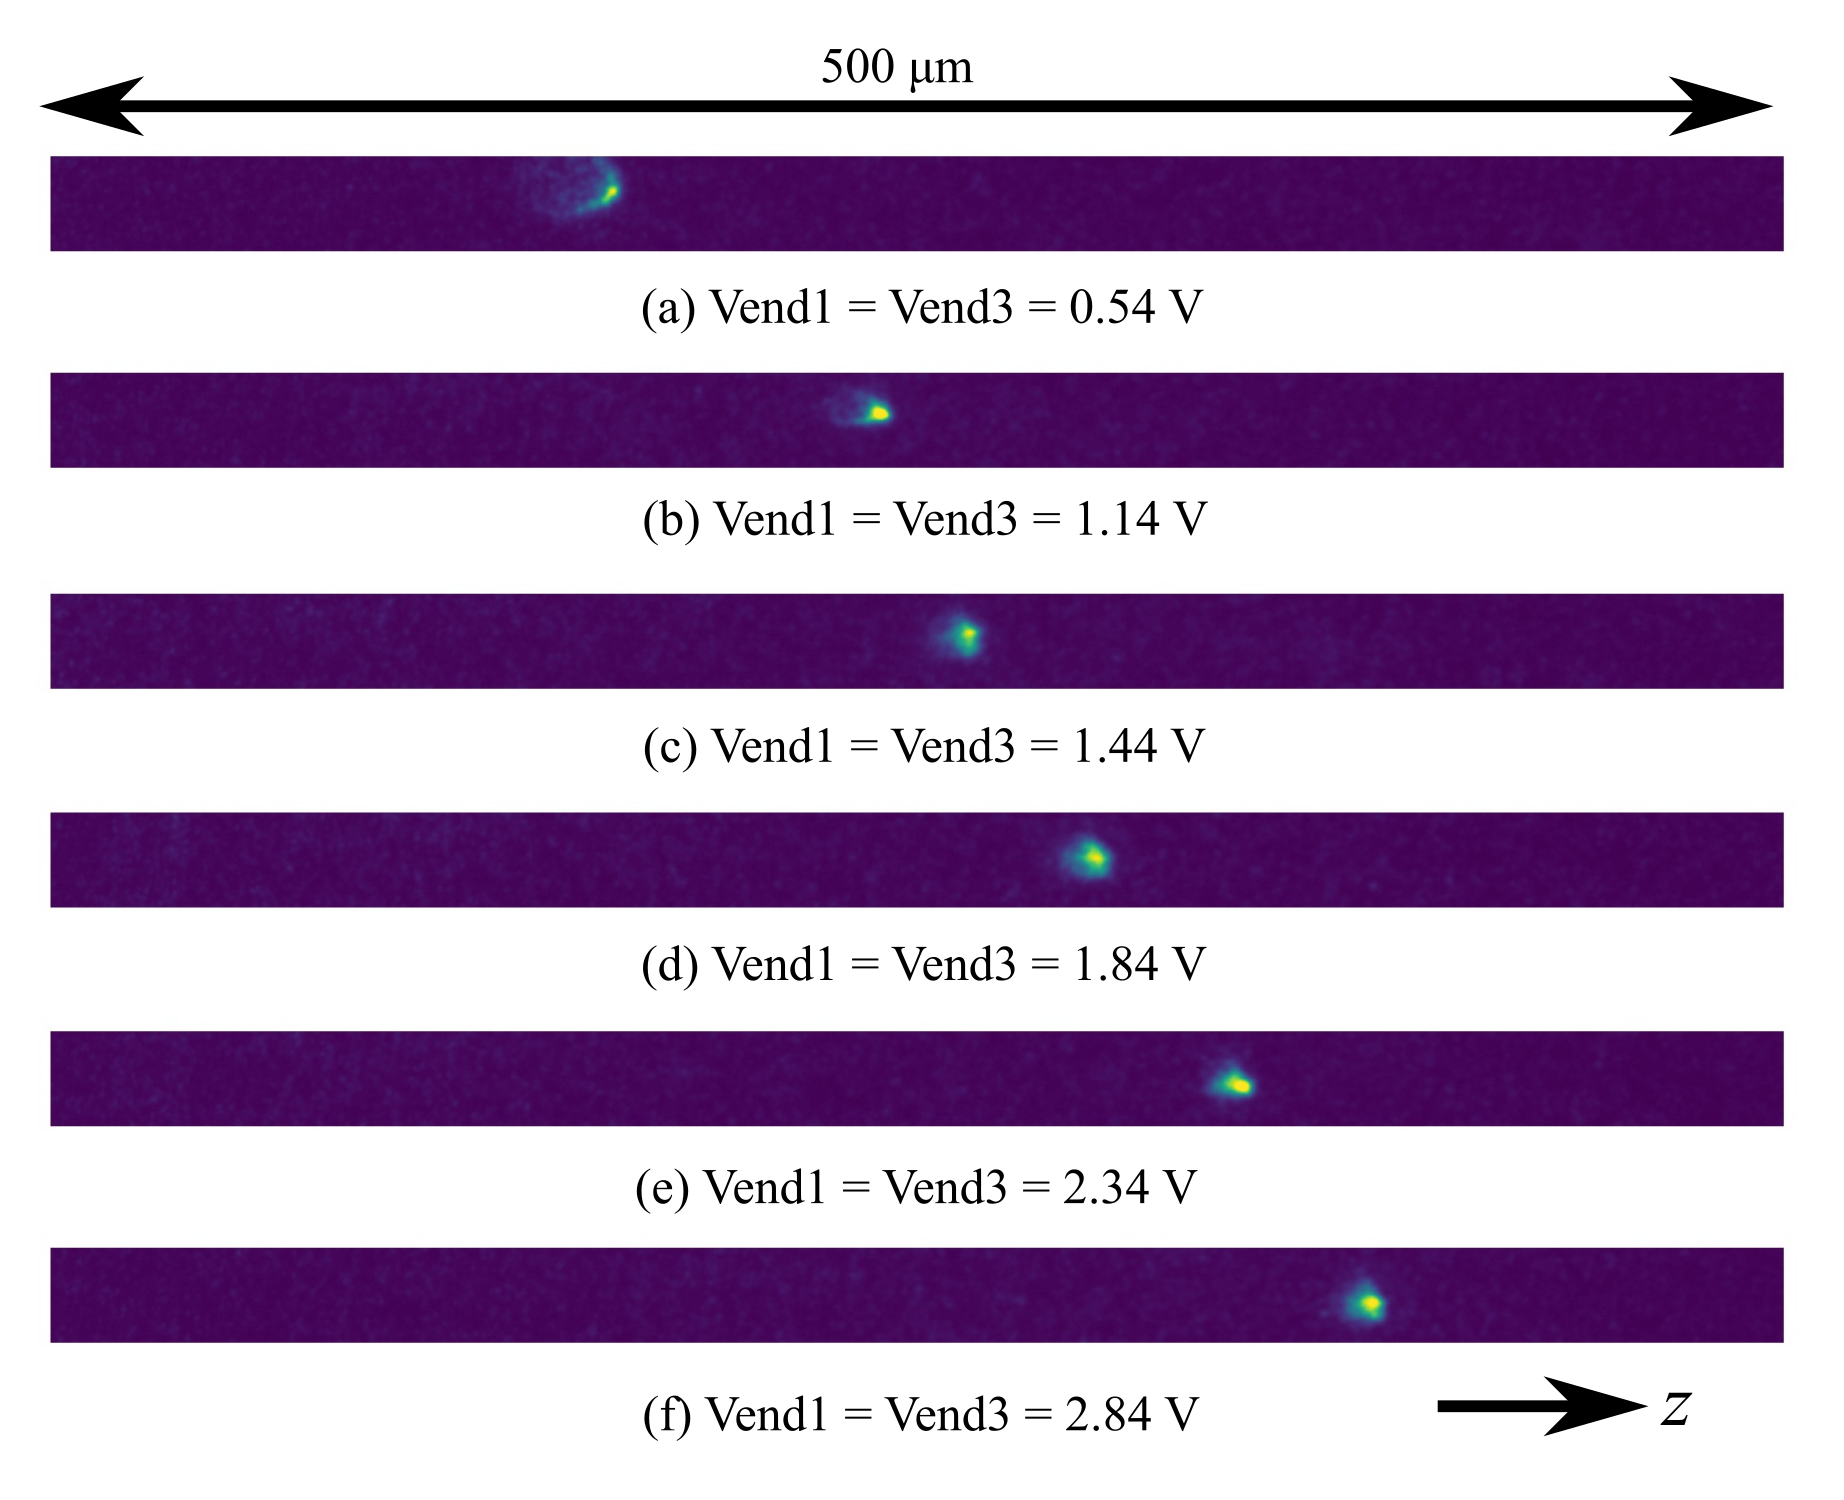
\includegraphics[width = 0.6 \linewidth]{./results/figure/displacement_End_Odd.png}
		\caption{$V_{\rm End1}, V_{\rm End3} = 0.54{\rm \ (a)}, \ 1.14{\rm \ (b)}, \ 1.44{\rm \ (c)}, \ 1.84{\rm \ (d)}, \ 2.34{\rm \ (e)}, \ 2.84{\rm \ (f)} \ {\rm V}$のときのイオン捕獲画像}
		\label{fig:displacement_End13}
	\end{center}
\end{figure}

\Fig{displacement_End13}より,End1とEnd3に印加するdc電圧を大きくしていくと$+z$方向へとイオン捕獲位置が変位し,dc電圧を小さくしていくと$-z$方向へ変位することが確認できた.
%
\clearpage
%
\Tb{dc_string}の条件におけるイオン捕獲位置を基準とし,$V_{\rm End1}, \ V_{\rm End3}$の変化に対するイオン捕獲位置の変位とシミュレーション上でのイオン捕獲位置の変位との比較を\Fig{sim_exp_displacement_End13}に示す.なお,シミュレーション上でのイオン捕獲位置は,プレーナートラップ電極モデルのx=0におけるSecularポテンシャルの最小値としている.
\begin{figure}[h]
	\begin{center}
		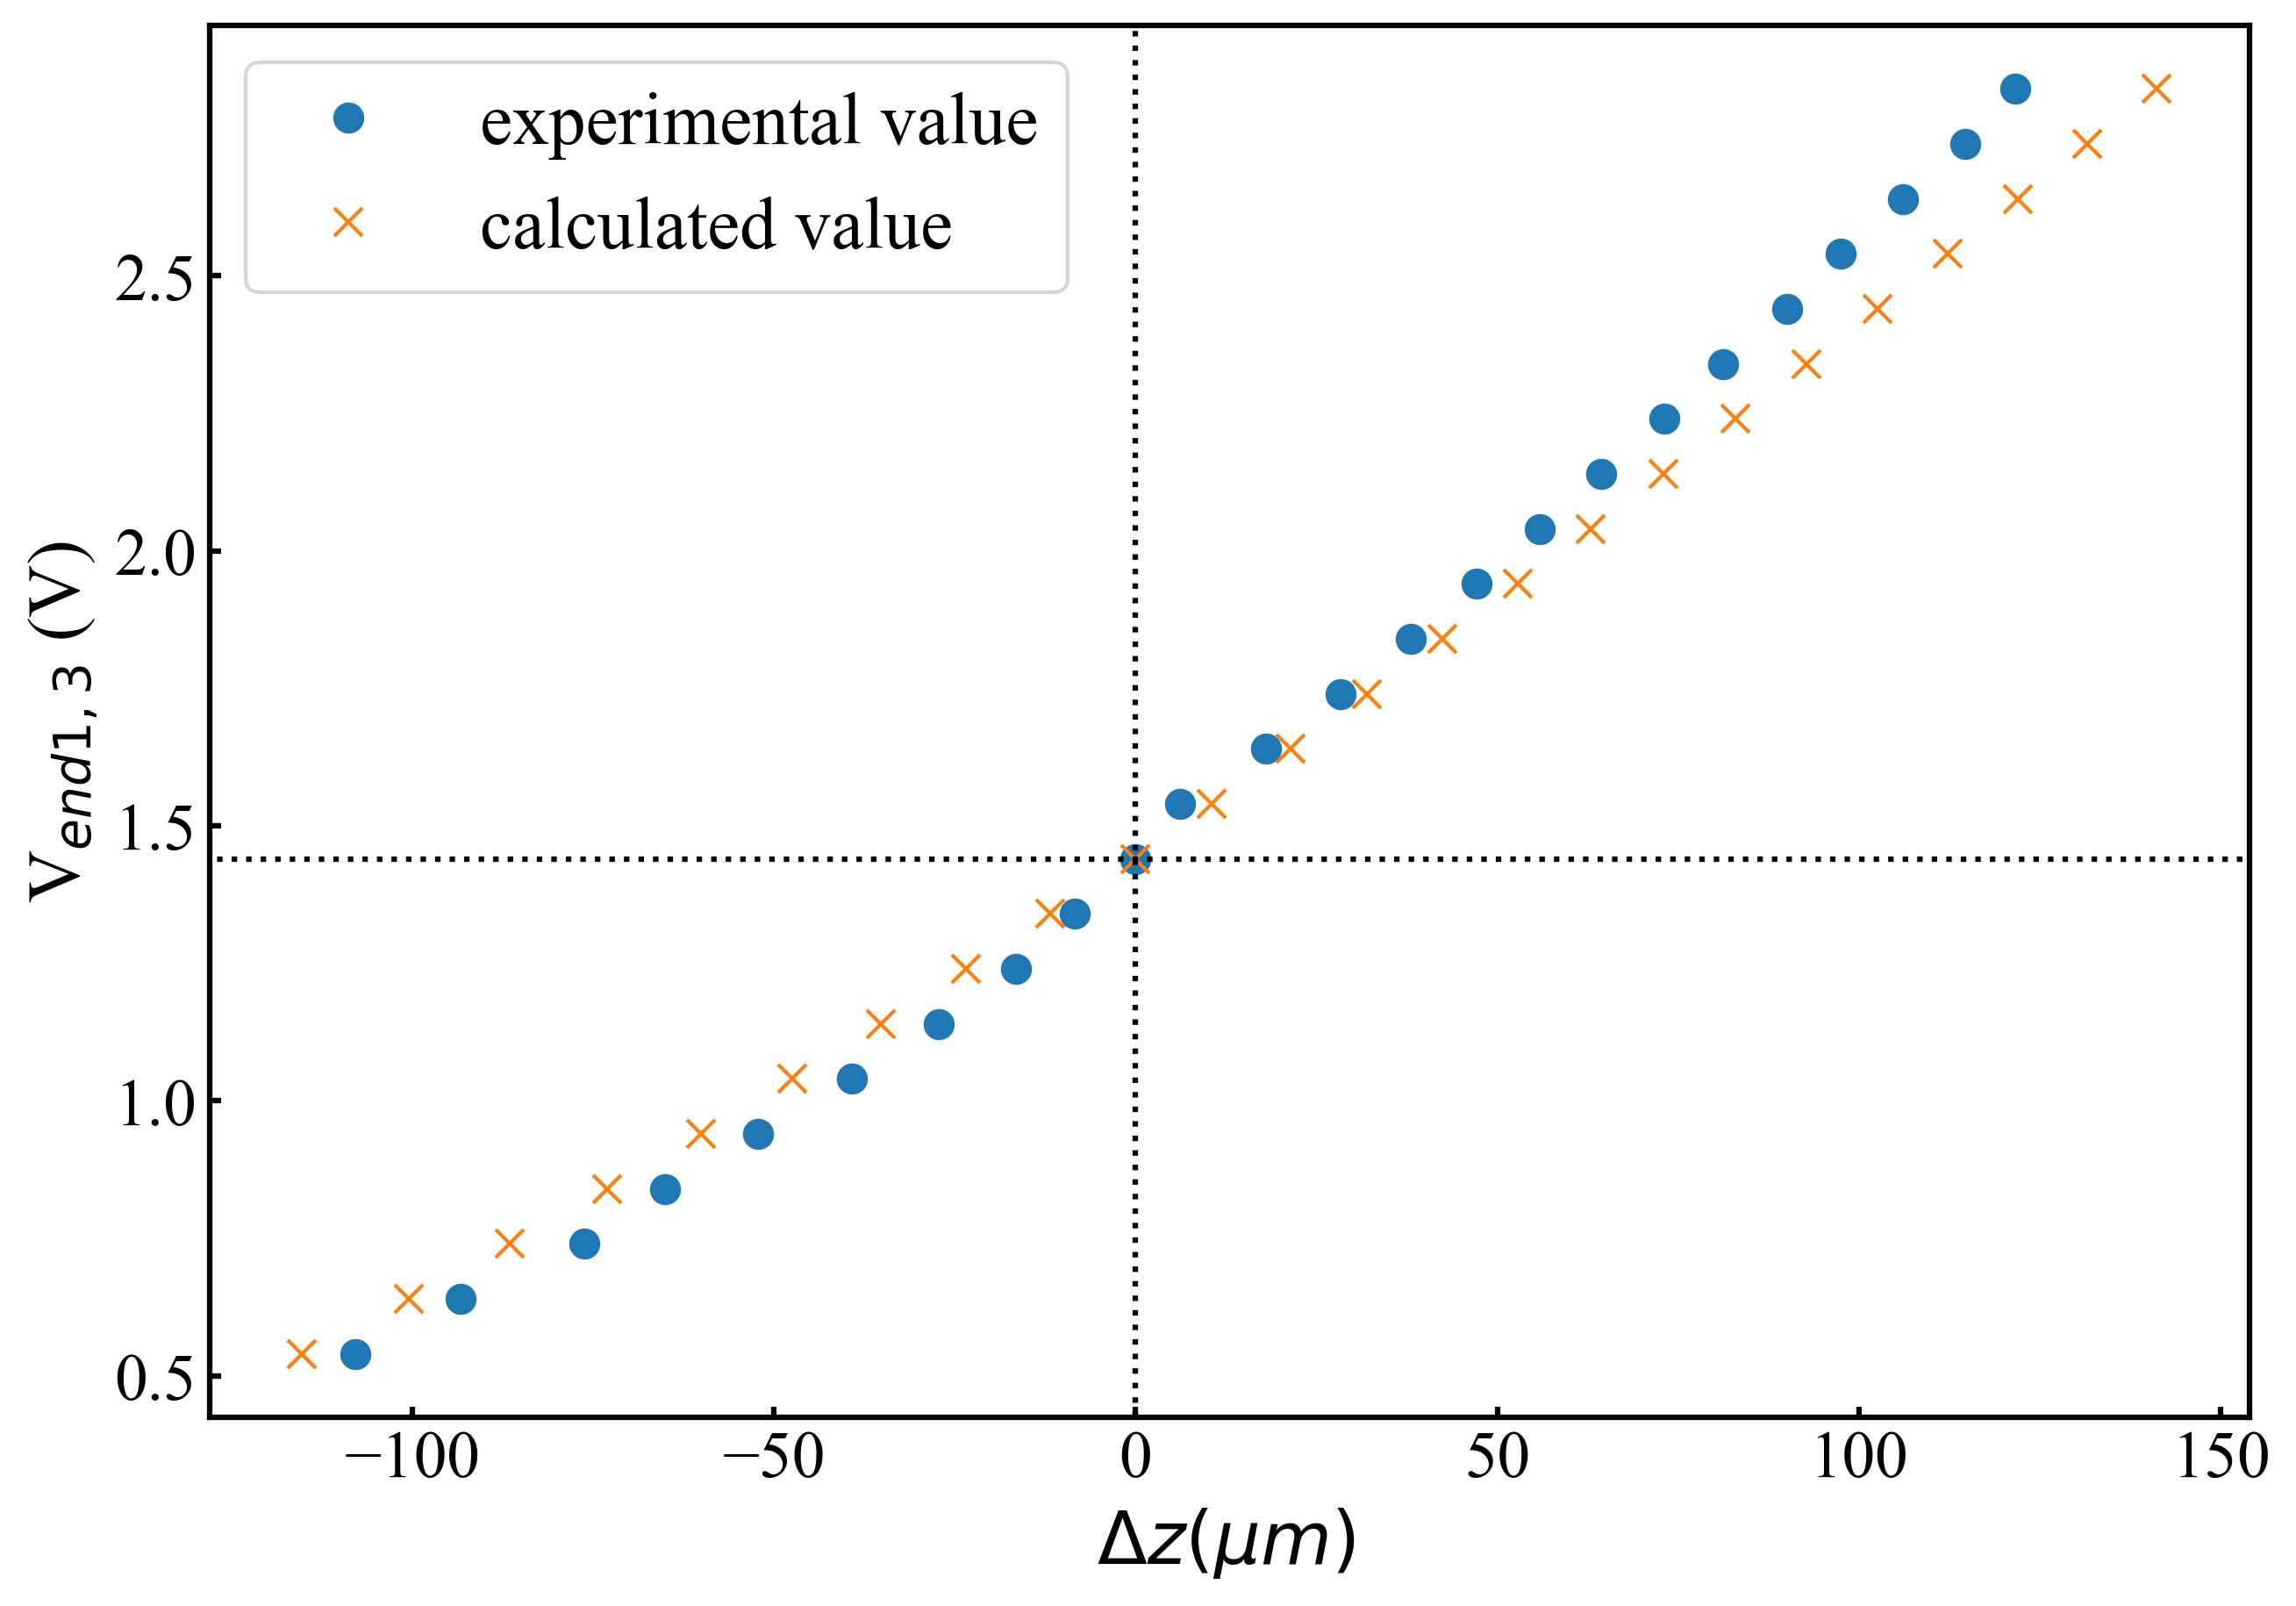
\includegraphics[width = 0.6\linewidth]{./results/figure/out_V13.jpg}
		\caption{\Tb{dc_string}の条件にて${\rm V}_{\rm End1}$と${\rm V}_{\rm End3}$の値を$0.54 \sim 2.84$Vまで0.1Vずつ変化させたときのイオン捕獲位置の変位の実験値とシミュレーション値との比較}
		\label{fig:sim_exp_displacement_End13}
	\end{center}
\end{figure}

$V_{\rm End2}, \ V_{\rm End4}$の電圧値を変化させて同様の実験を行った.実験値とシミュレーション値との比較を\Fig{sim_exp_displacement_End24}に示す.

\begin{figure}[h]
	\begin{center}
		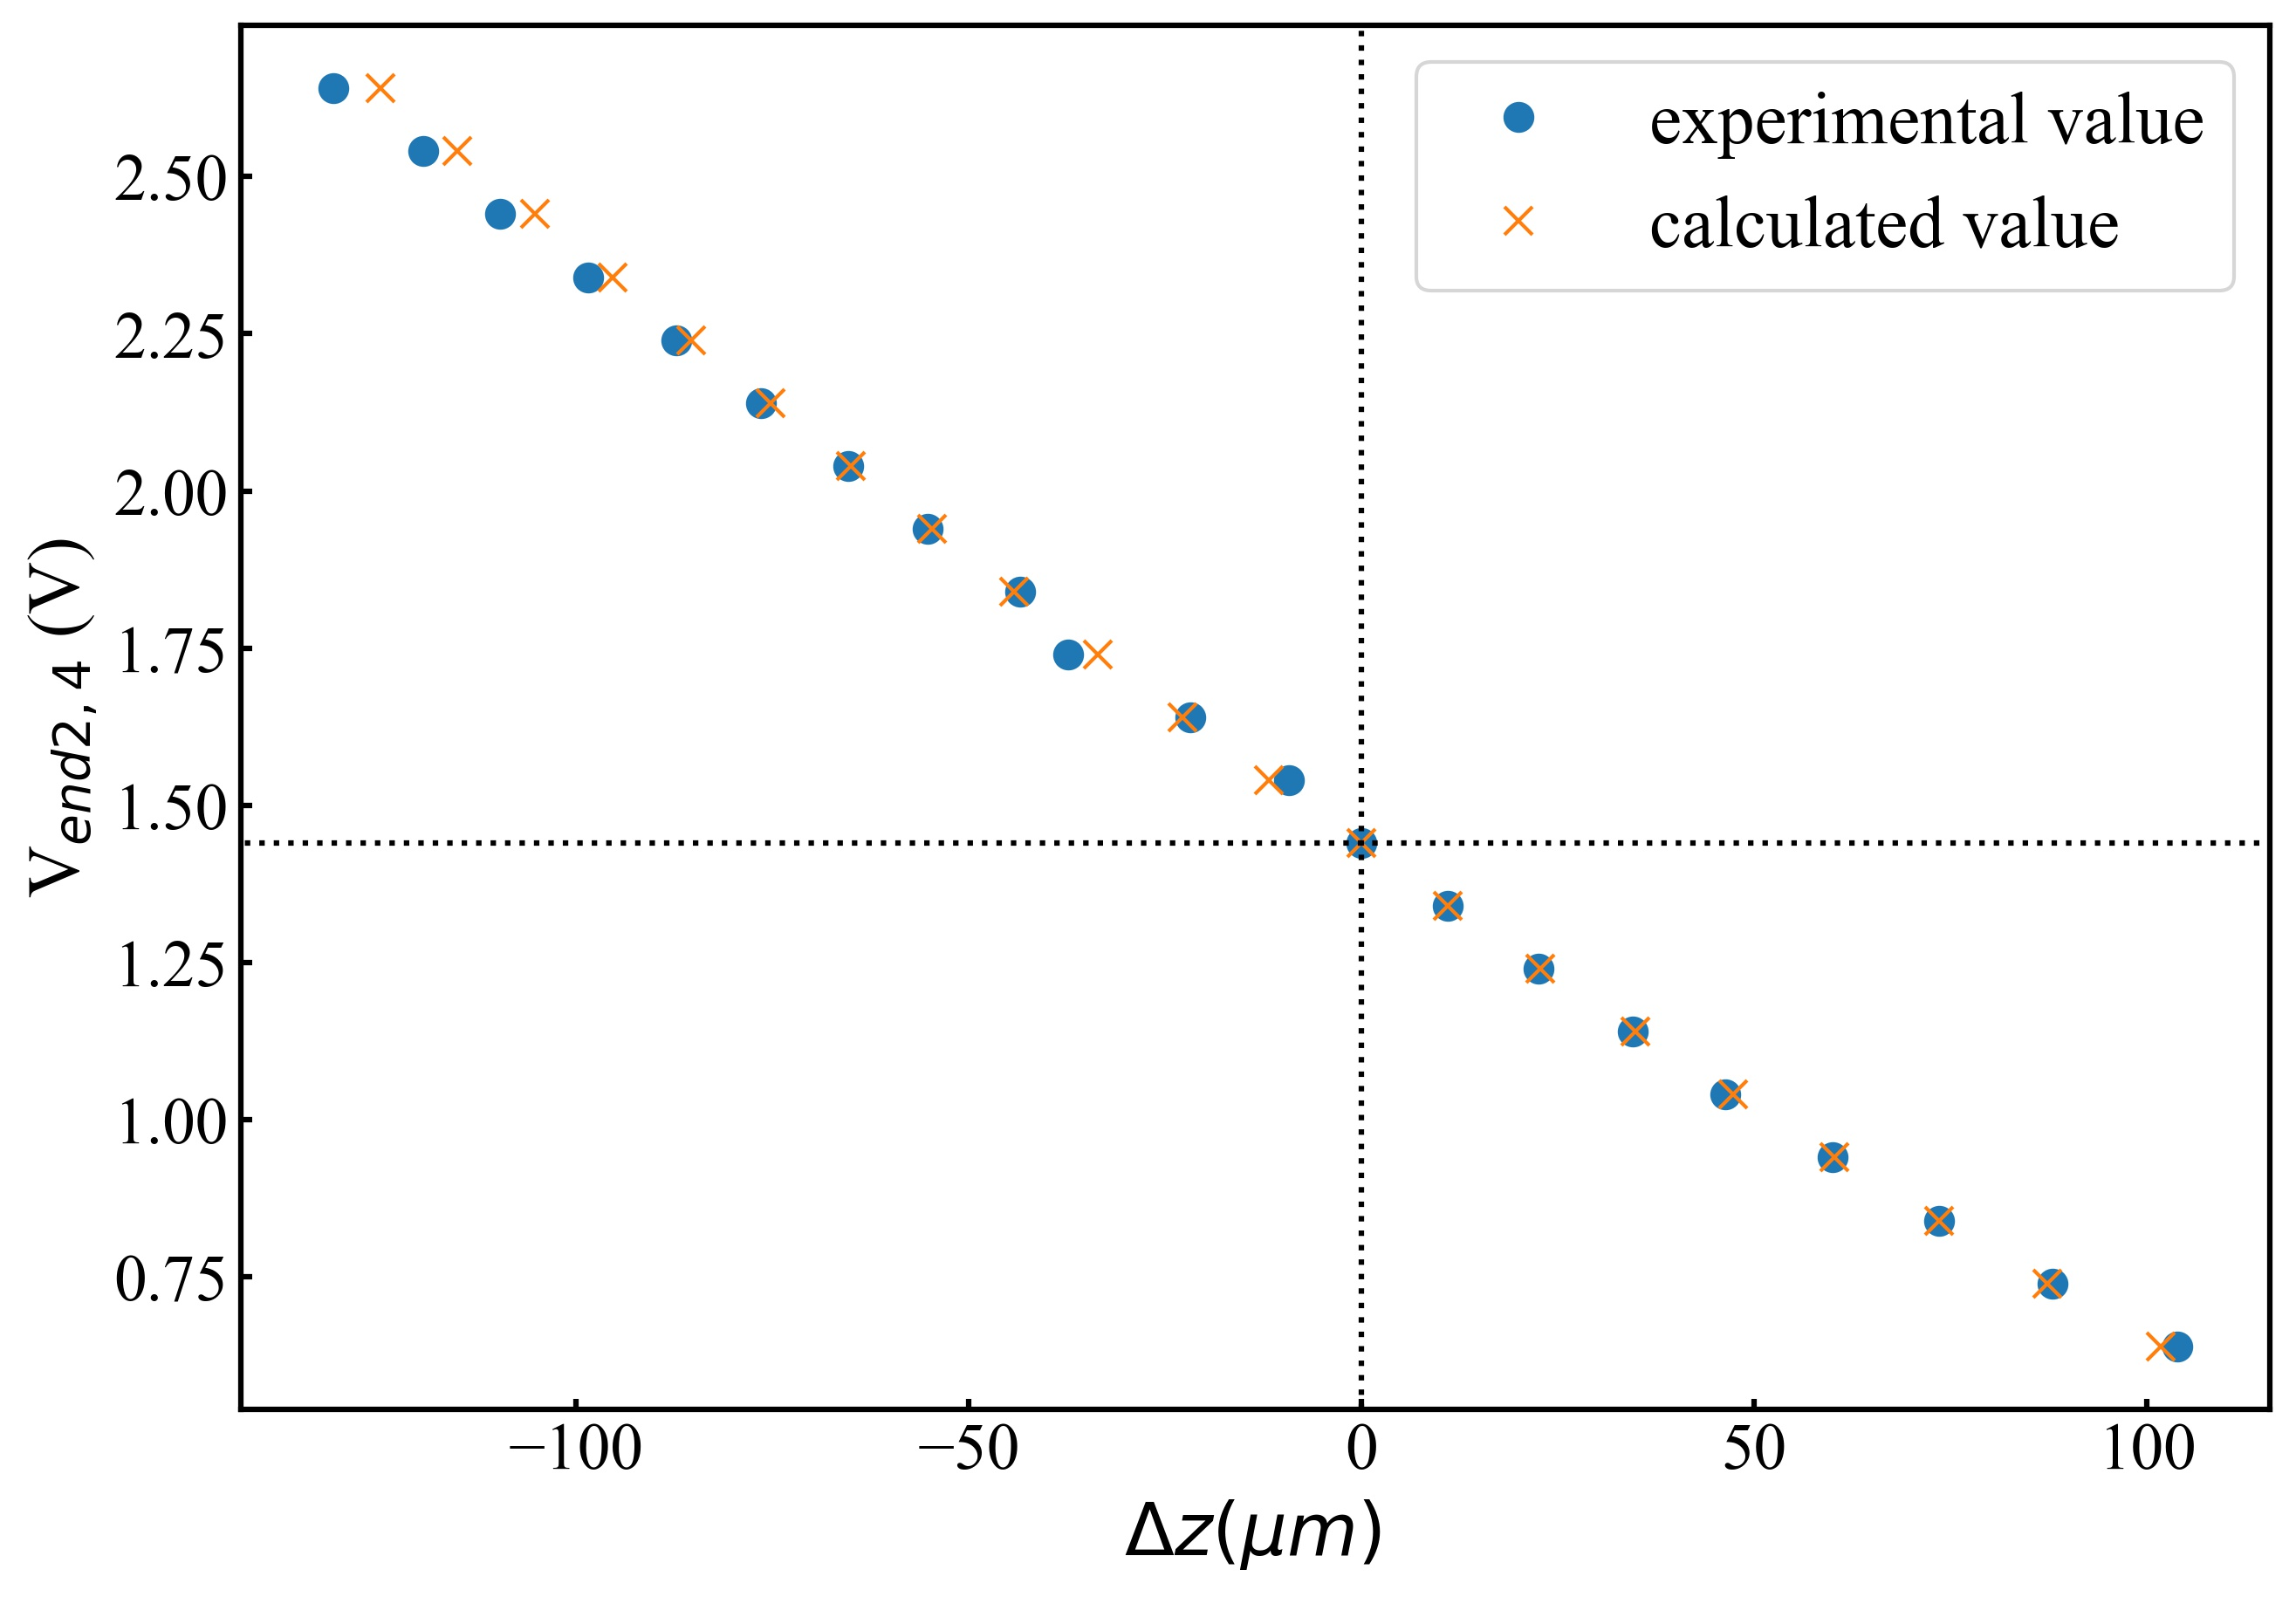
\includegraphics[width = 0.6\linewidth]{./results/figure/out_V24.jpg}
		\caption{\Tb{dc_string}の条件にて${\rm V}_{\rm End2}$と${\rm V}_{\rm End4}$の値を$0.54 \sim 2.84$Vまで0.1Vずつ変化させたときのイオン捕獲位置の変位の実測値とシミュレーション値との比較}
			\label{fig:sim_exp_displacement_End24}
	\end{center}
\end{figure}

\Fig{sim_exp_displacement_End24}より,End2とEnd4に印加するdc電圧を大きくしていくと$-z$方向へイオン捕獲位置が変位し,dc電圧を小さくしていった場合に$+z$方向へ変位することが確認できた.

\clearpage

\subsection{永年周波数のdc電圧依存性}
\ref{MeasSecFreq_Method}に示した手法を用いて,単一イオンを用いて異なるdc電圧セットにおける永年周波数の測定を行い,シミュレーション値との比較を行った.\Fig{end13_MeasSec}に\Tb{dc_string}に示すdc電圧セットを基準として$V_{\rm End1}, \ V_{\rm End3}$を変化させたときのイオンの振幅の周波数特性を示す.各条件に対し共鳴現象を引き起こすac信号の振幅は200$\ {\rm mV_{pp}}$とし,周波数掃引の刻み幅は50$\ {\rm Hz}$としている.周波数掃引の範囲は,まず手動で周波数を変化させ,共鳴現象が確認される周波数から$\pm1.5 \ {\rm kHz}$程度の範囲としイオンの振幅の周波数特性の取得を行った.

\begin{figure}[h]
	\begin{center}
		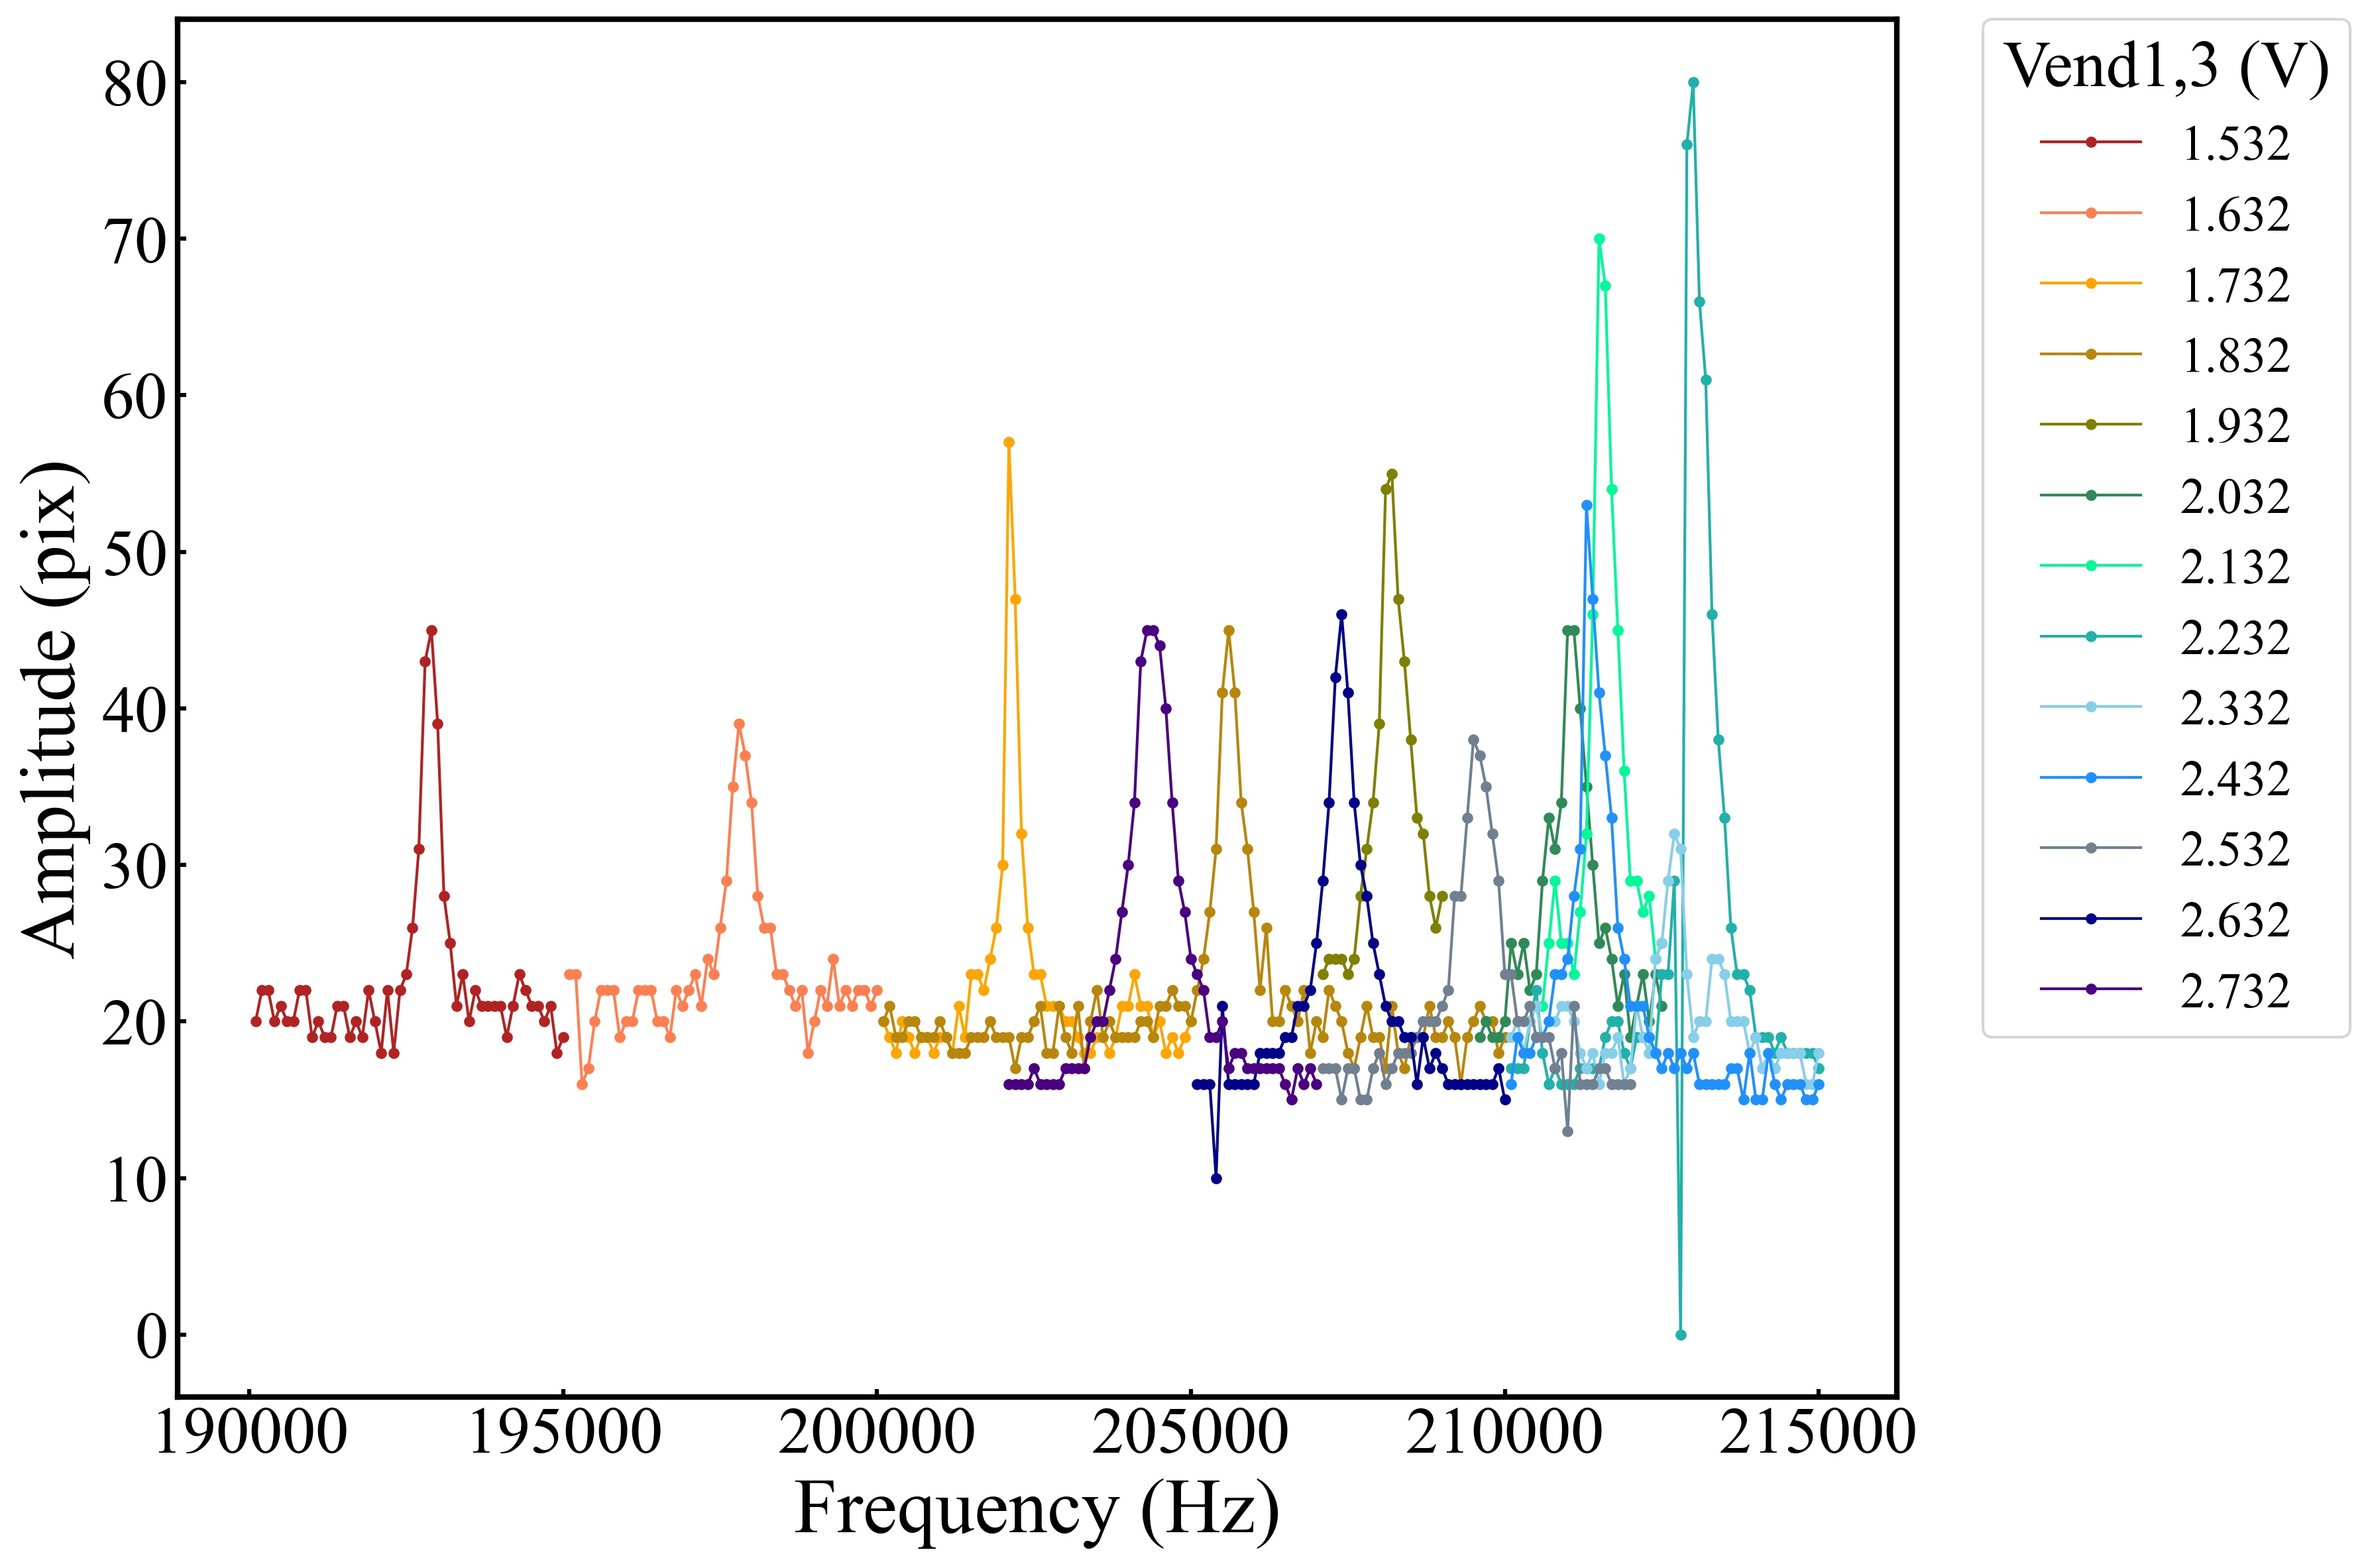
\includegraphics[width = 0.6\linewidth]{./results/figure/end13-SecFreq.jpg}
		\caption{$V_{\rm End1}$と$V_{\rm End3}$を変化させたときのイオンの振幅の周波数特性}
		\label{fig:end13_MeasSec}
	\end{center}
\end{figure}

\Fig{end13_MeasSec}より,それぞれのイオンの振幅の周波数特性をローレンツ分布関数によるフィッティングを行い,永年周波数の決定を行った.フィッティングで得られた永年周波数とシミュレーションから計算された永年周波数との比較を\Fig{end13_MeasSec_SimSec}に示す.

\begin{figure}[h]
	\begin{center}
		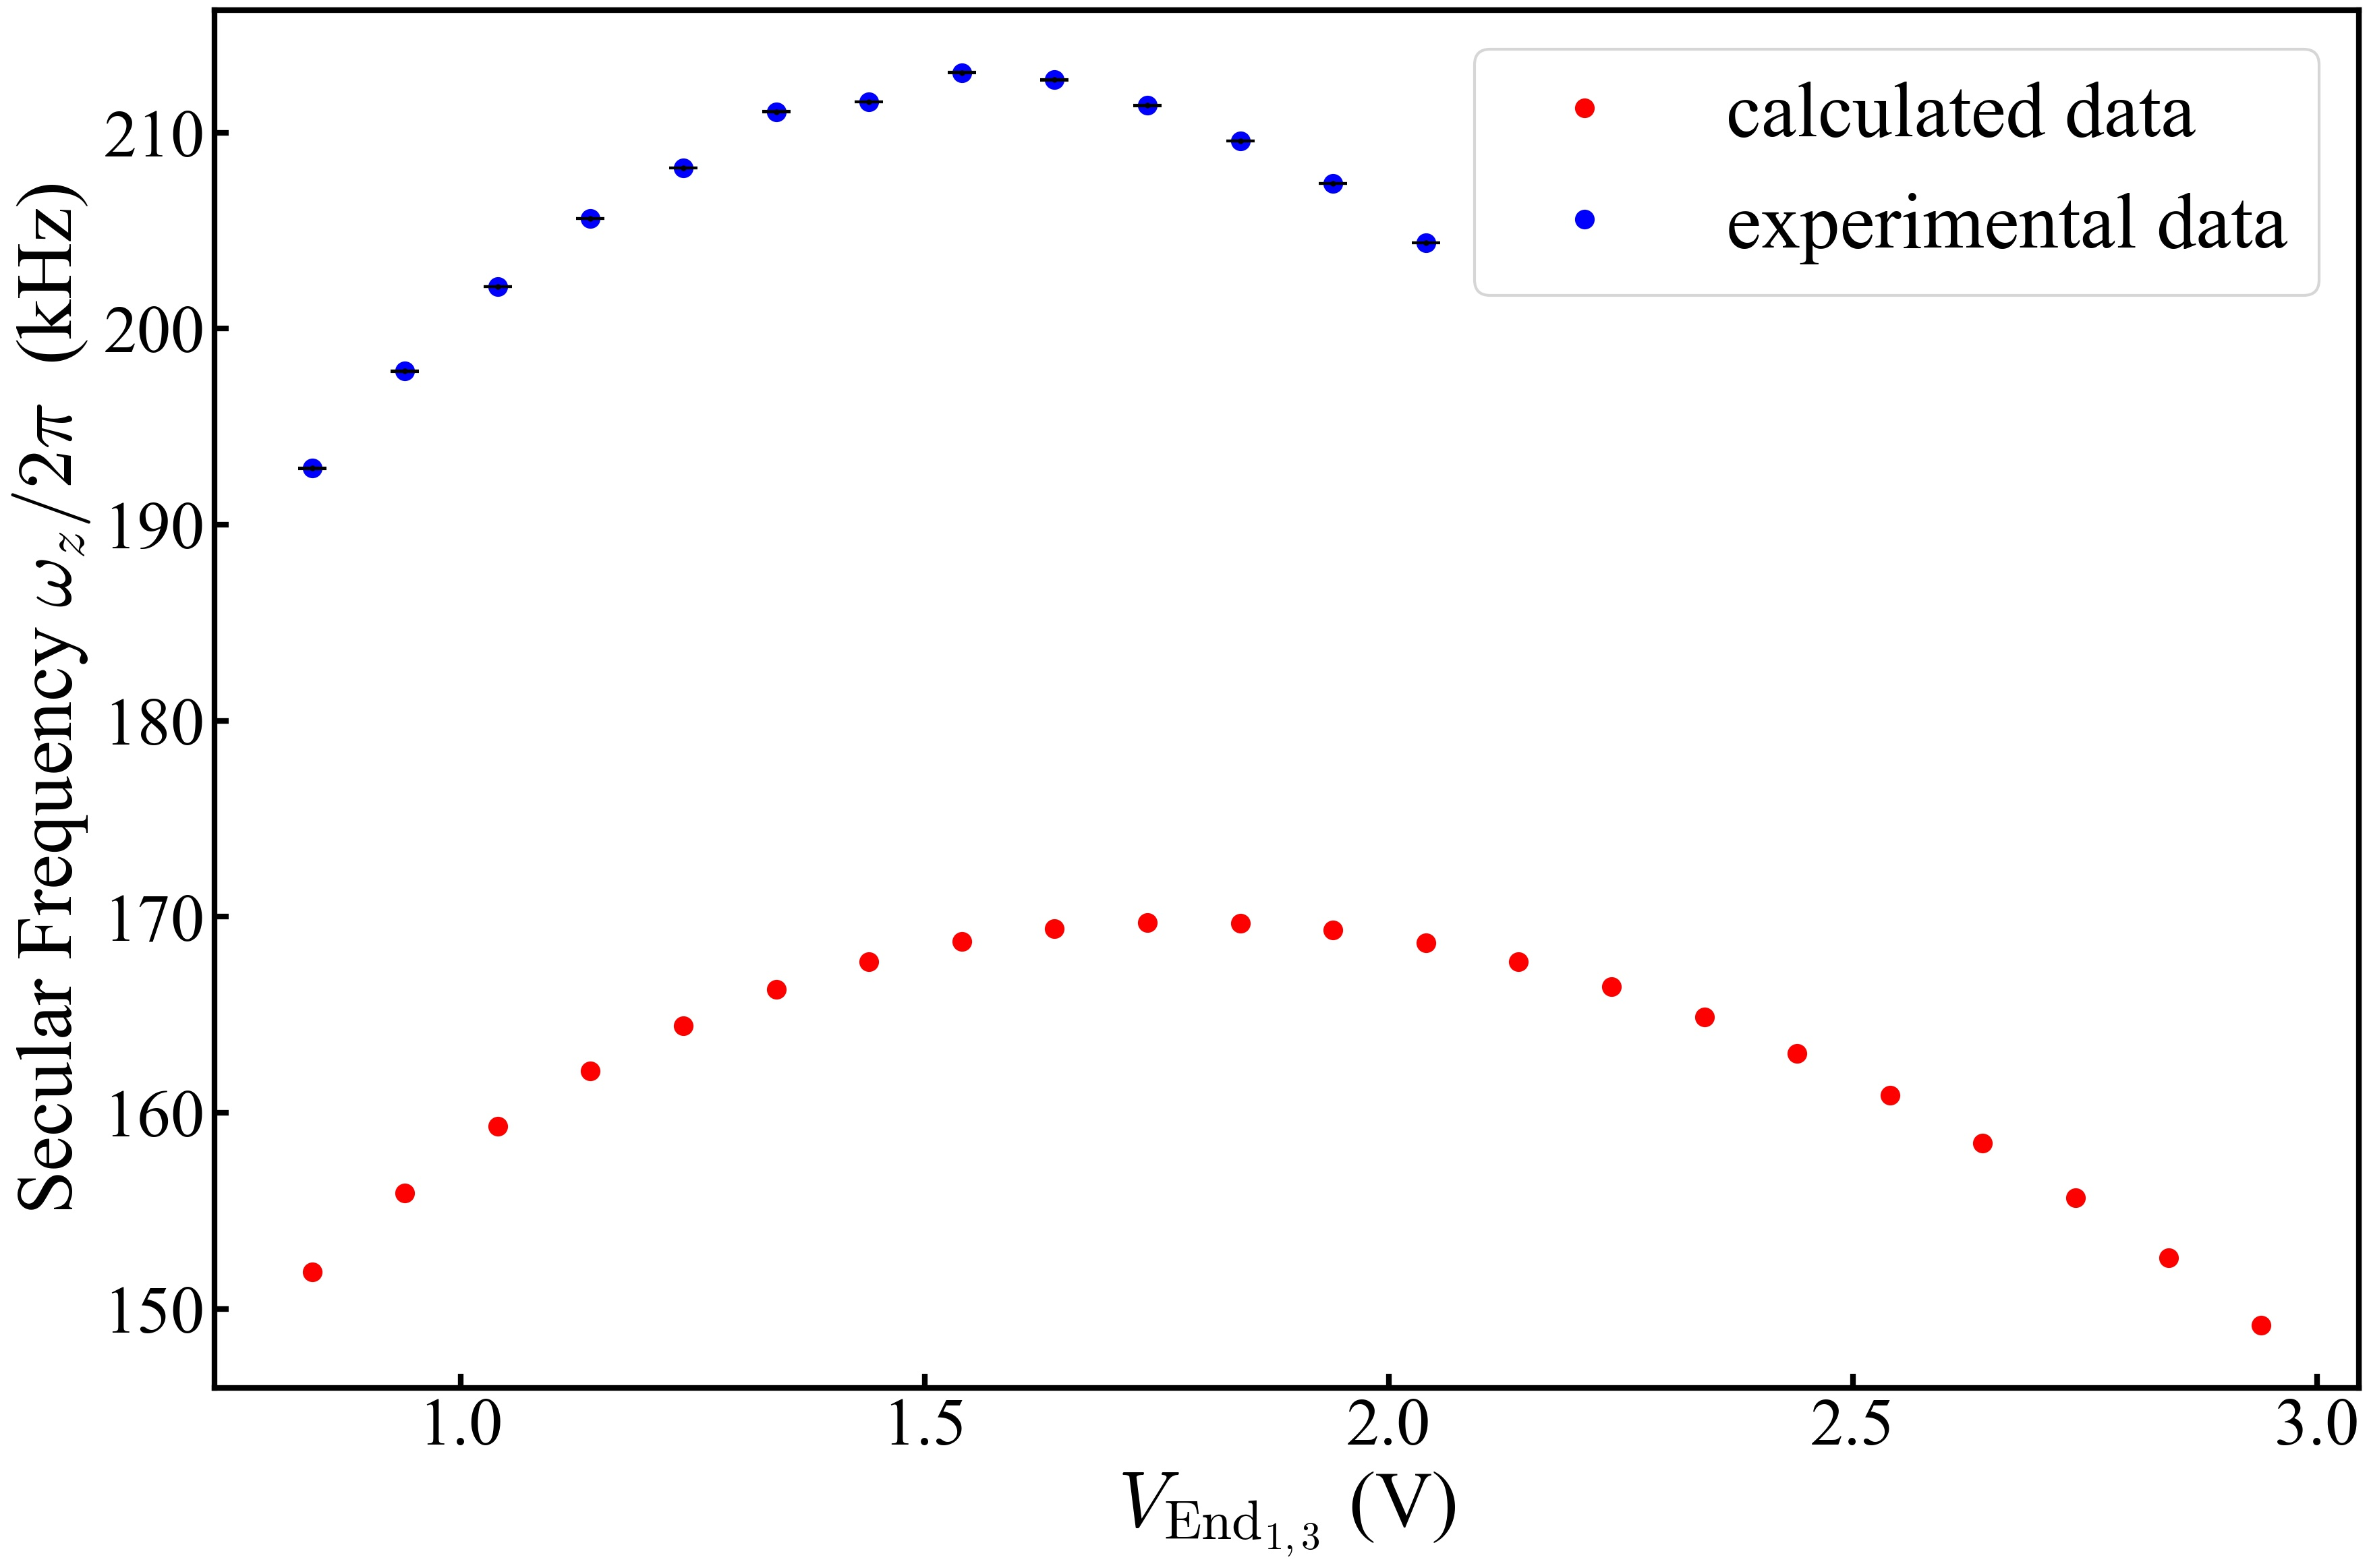
\includegraphics[width = 0.6\linewidth]{./results/figure/Vend13-SecFreqZ.jpg}
		\caption{$V_{\rm End1}$と$V_{\rm End3}$を変化させたときの永年周波数の測定結果とシミュレーション結果との比較}
		\label{fig:end13_MeasSec_SimSec}
	\end{center}
\end{figure}

\Fig{end13_MeasSec_SimSec}より,測定値とシミュレーション値との差が$35.726 \ {\rm kHz} \ \sim 44.771 \ {\rm kHz}$の範囲で存在することが分かる.また,永年周波数の$V_{\rm End1}$と$V_{\rm End3}$依存性における極値を取る$V_{\rm End1}, \ V_{\rm End3}$が異なっていることが分かる.
%
\clearpage
%
次に,$V_{\rm End2}$と$V_{\rm End4}$を変化させ,同様の手順で永年周波数の測定を行った.このときのイオンの振幅の周波数特性を\Fig{end24_MeasSec}に示す.

\begin{figure}[h]
	\begin{center}
		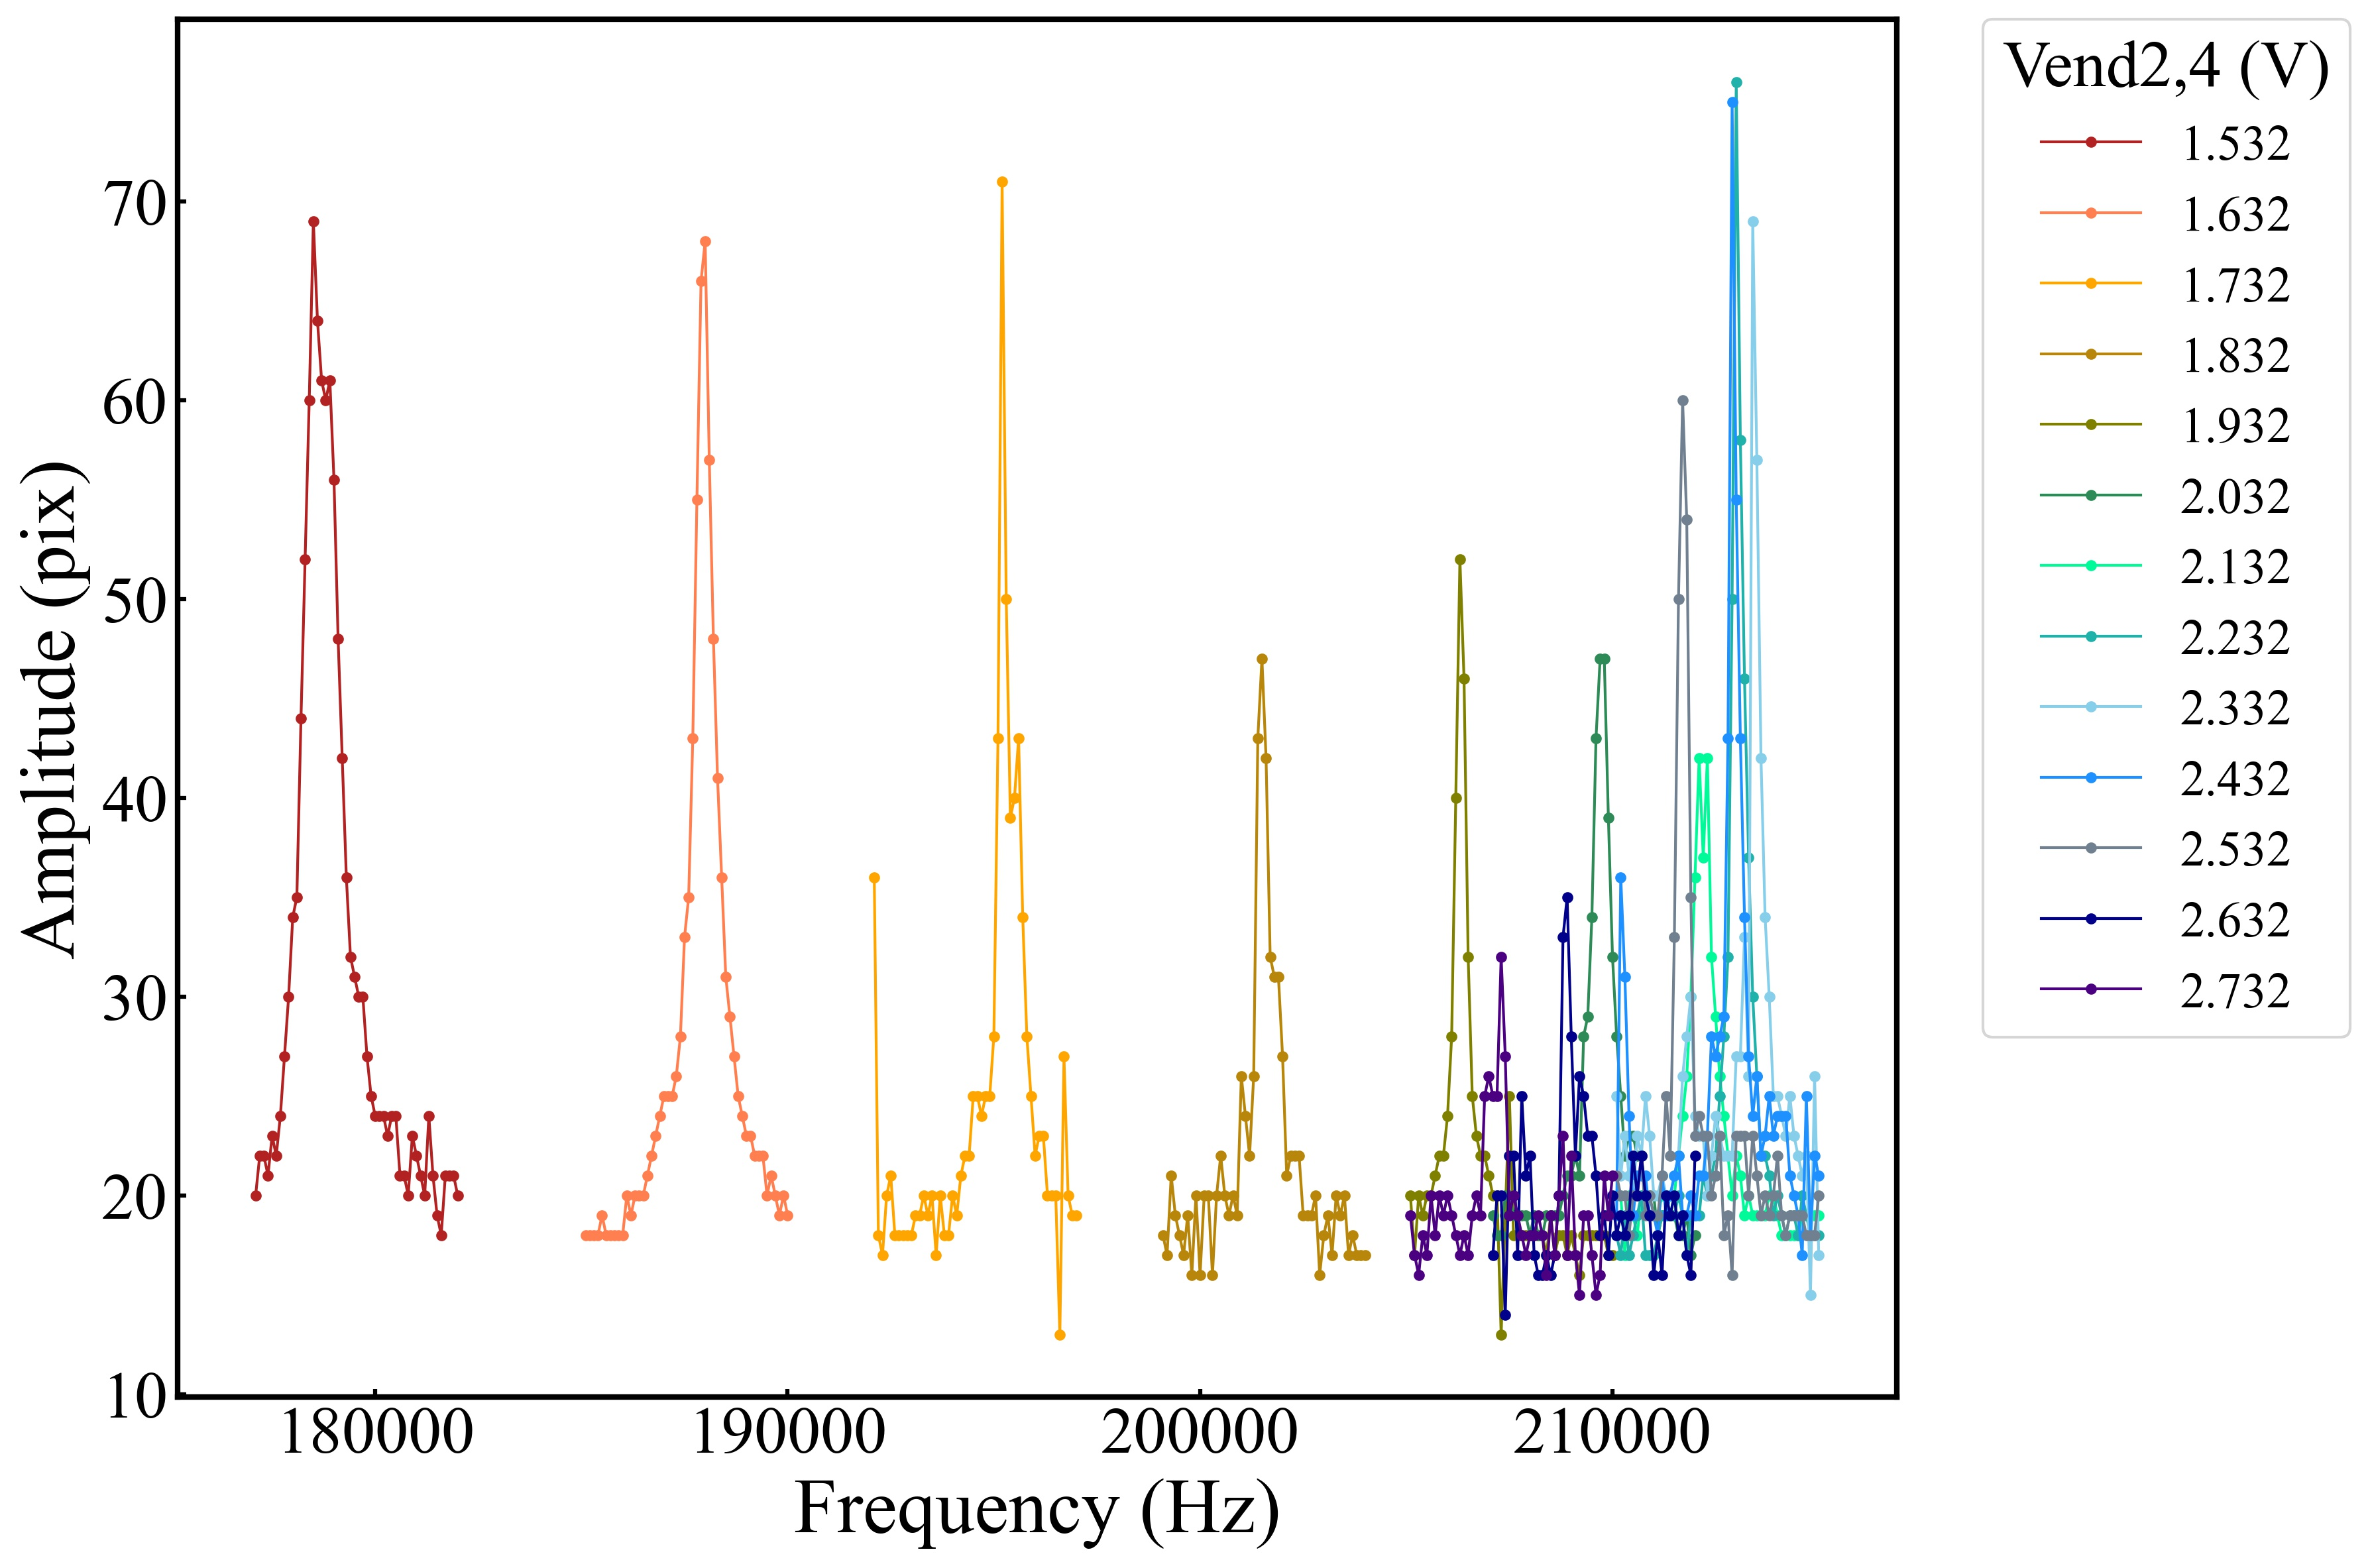
\includegraphics[width = 0.6\linewidth]{./results/figure/end24-SecFreq.jpg}
		\caption{$V_{\rm End2}$と$V_{\rm End4}$を変化させたときのイオンの振幅の周波数特性}
		\label{fig:end24_MeasSec}
	\end{center}
\end{figure}

\Fig{end24_MeasSec}より,ローレンツ分布関数によるフィッティングから得られた永年周波数とシミュレーションから得られた永年周波数との比較を\Fig{end24_MeasSec_SimSec}に示す.

\begin{figure}[h]
	\begin{center}
		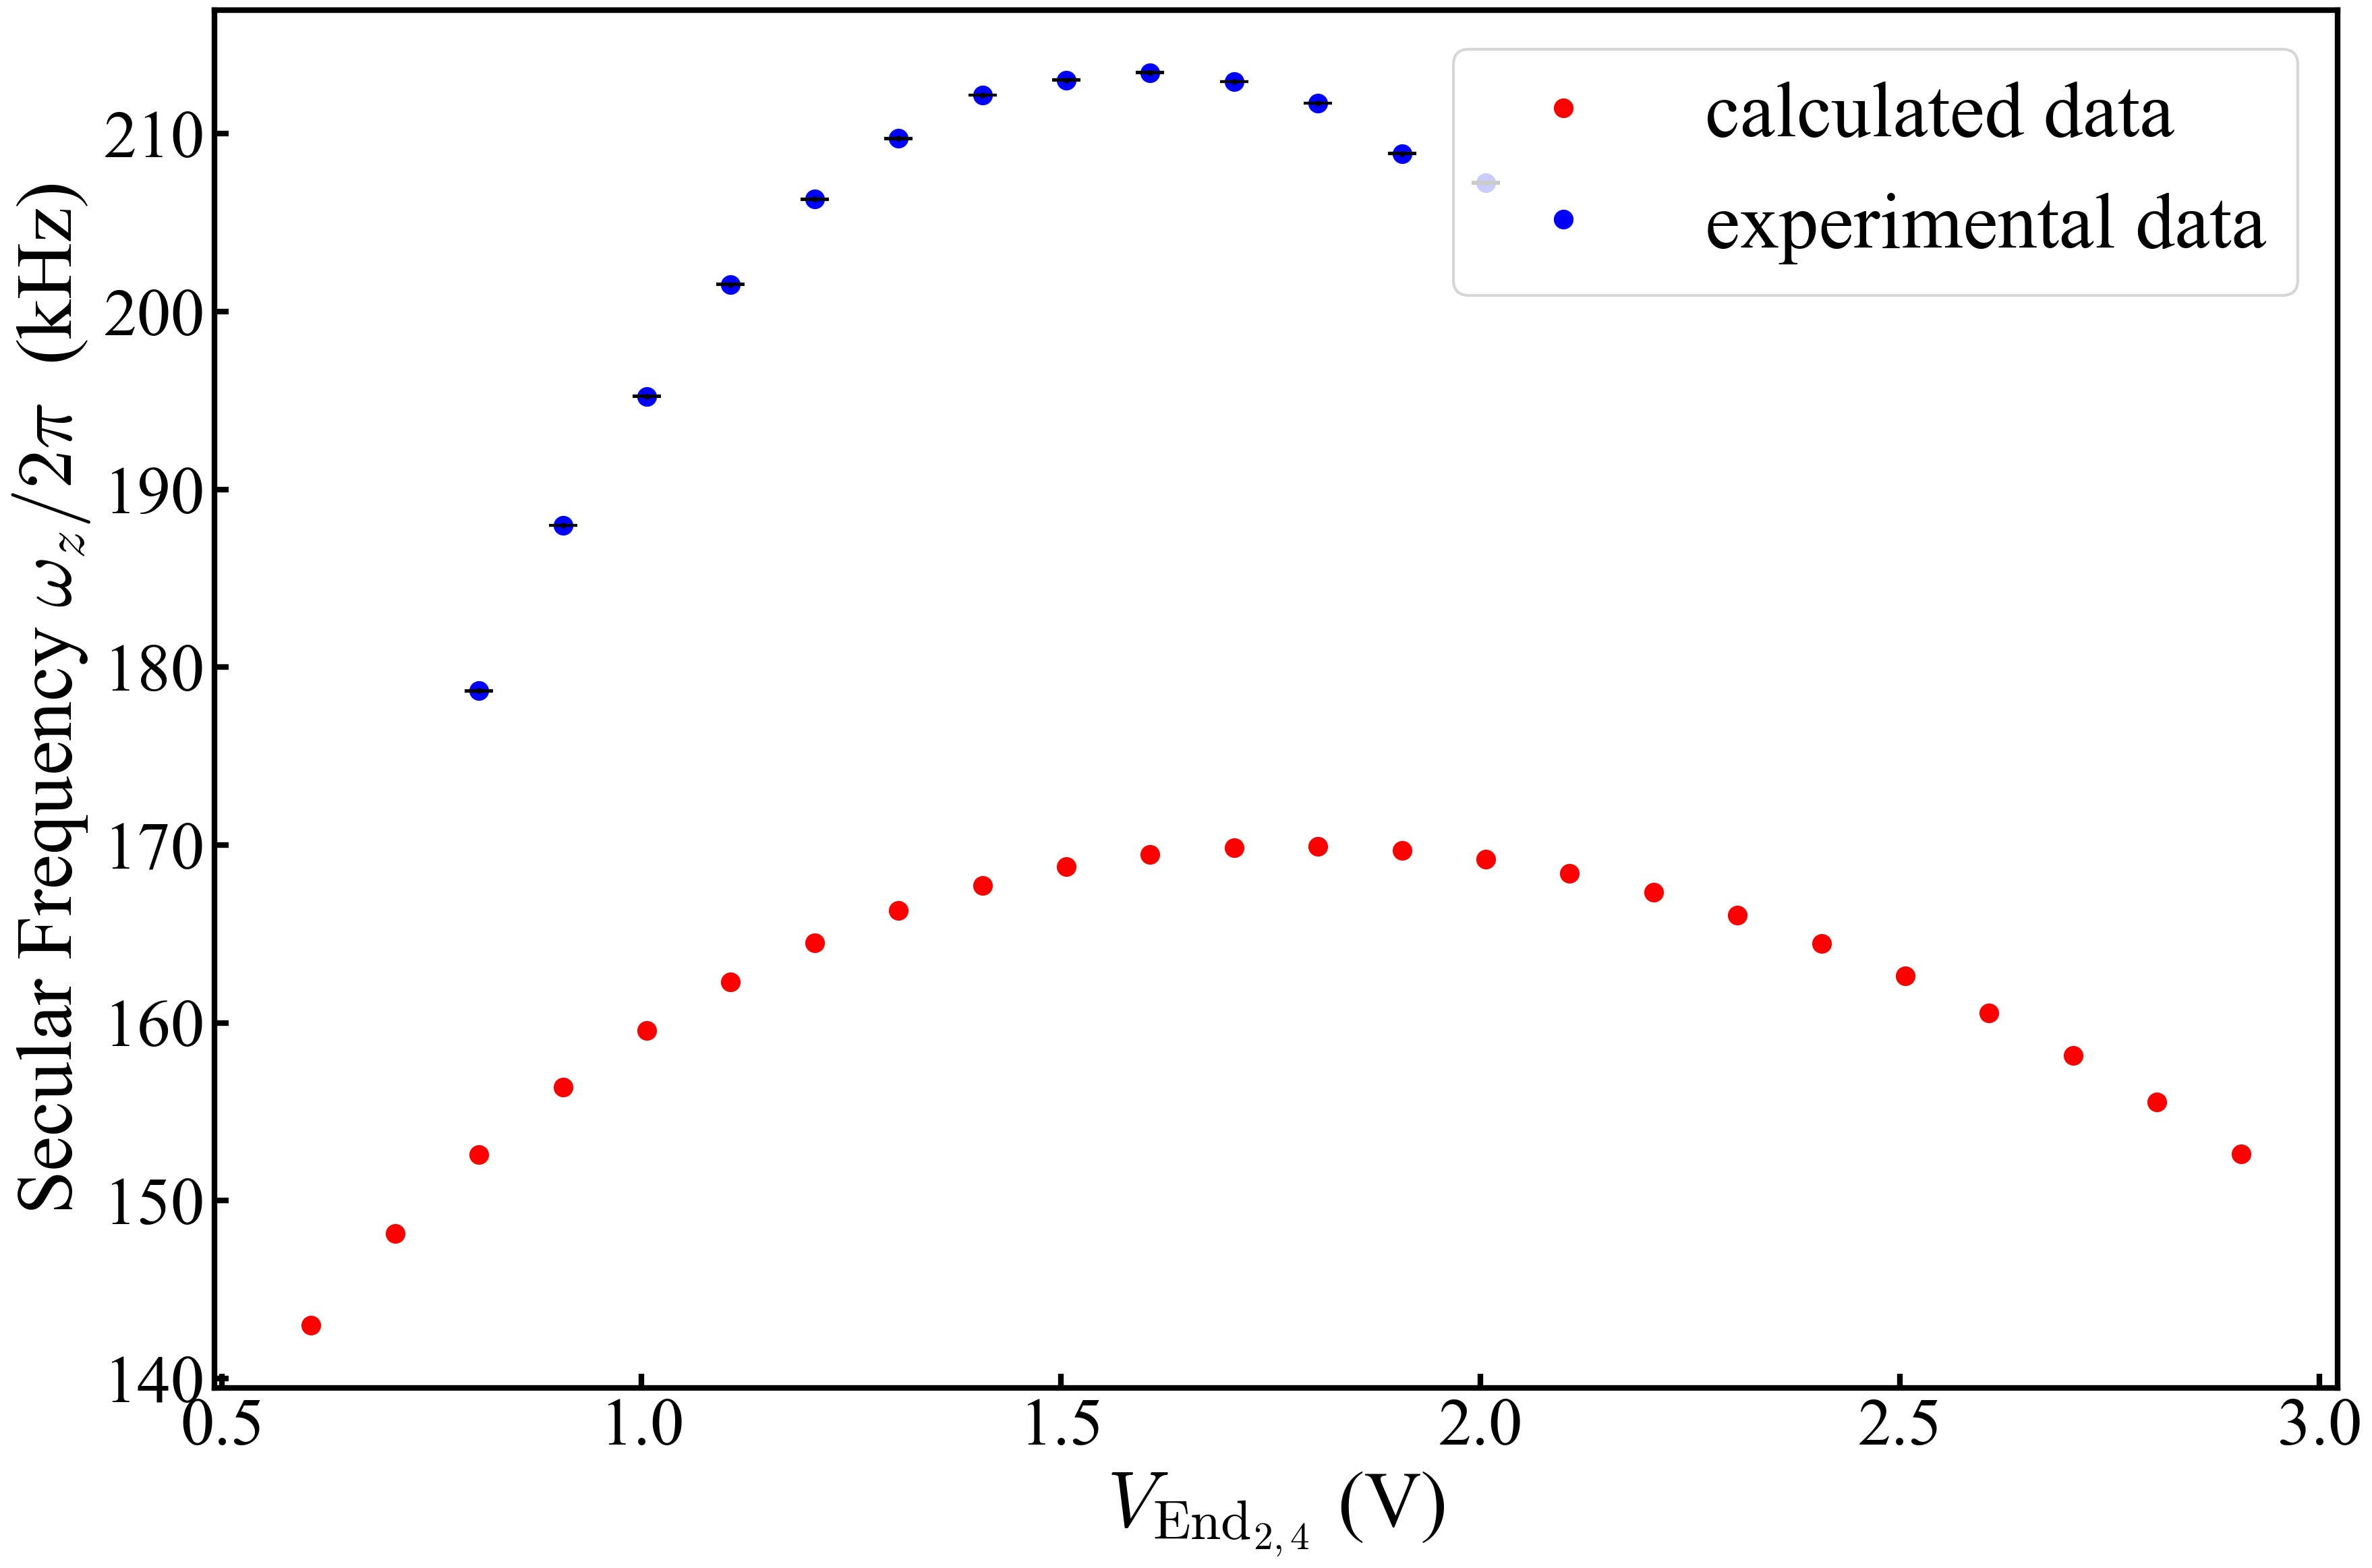
\includegraphics[width = 0.6\linewidth]{./results/figure/Vend24-SecFreqZ.jpg}
		\caption{$V_{\rm End2}$と$V_{\rm End4}$を変化させたときの永年周波数の測定結果とシミュレーション結果との比較}
		\label{fig:end24_MeasSec_SimSec}
	\end{center}
\end{figure}

\Fig{end24_MeasSec_SimSec}から,実験値とシミュレーション値に$26.1 \ {\rm kHz} \ \sim \ 44.5 \ {\rm kHz}$の差があることが分かった.また,$V_{\rm End1}, \ V_{\rm End3}$に対して変化する永年周波数と同様に実験値とシミュレーション値のそれぞれが極値を取る$V_{\rm End2}, \ V_{\rm End4}$が異なることが分かる.
%
\clearpage
%
永年周波数の測定に際し,\Tb{dc_string}に示すdc電圧セットを基準としてきたが,固定するdc電圧と変化させるdc電圧との相対的な関係が変化すれば,変化させるdc電圧に対するイオンの応答性も異なってくる.そのため,各dc電極に印加するdc電圧の絶対値を評価量として採用せず,その代わりにdc電圧の比率の導入を行った.ここでは,$V_{\rm End1,3}$と$V_{\rm End2,4}$の比率fを
\large
\begin{align}
f = \frac{V_{\rm End1,3}}{V_{\rm End2,4}}
\end{align}
\normalsize
として導入し,永年周波数のdc電圧依存性の評価を行った.$V_{\rm End2,4}$を$1.106 \ {\rm V} \ \sim \ 1.706 \ {\rm V}$まで$0.1 \ {\rm V}$ずつ変化させ,$V_{\rm End2,4}$の各電圧値において,$V_{\rm End1,3}$を$0.84 \ {\rm V} \ \sim \ 2.14 \ {\rm V}$まで$0.1 \ {\rm V}$ずつ変化させ,各dc電圧値に対する永年周波数の測定を単一イオンを用いて行った.その結果を\Fig{Vendodd_Vendeven}に示す.また,\Fig{Vendodd_Vendeven}より,永年周波数のf特性を\Fig{Vendodd_Vendeven_f}に示す.
\begin{figure}[h]
	\begin{minipage}{0.5\linewidth}
		\begin{center}
			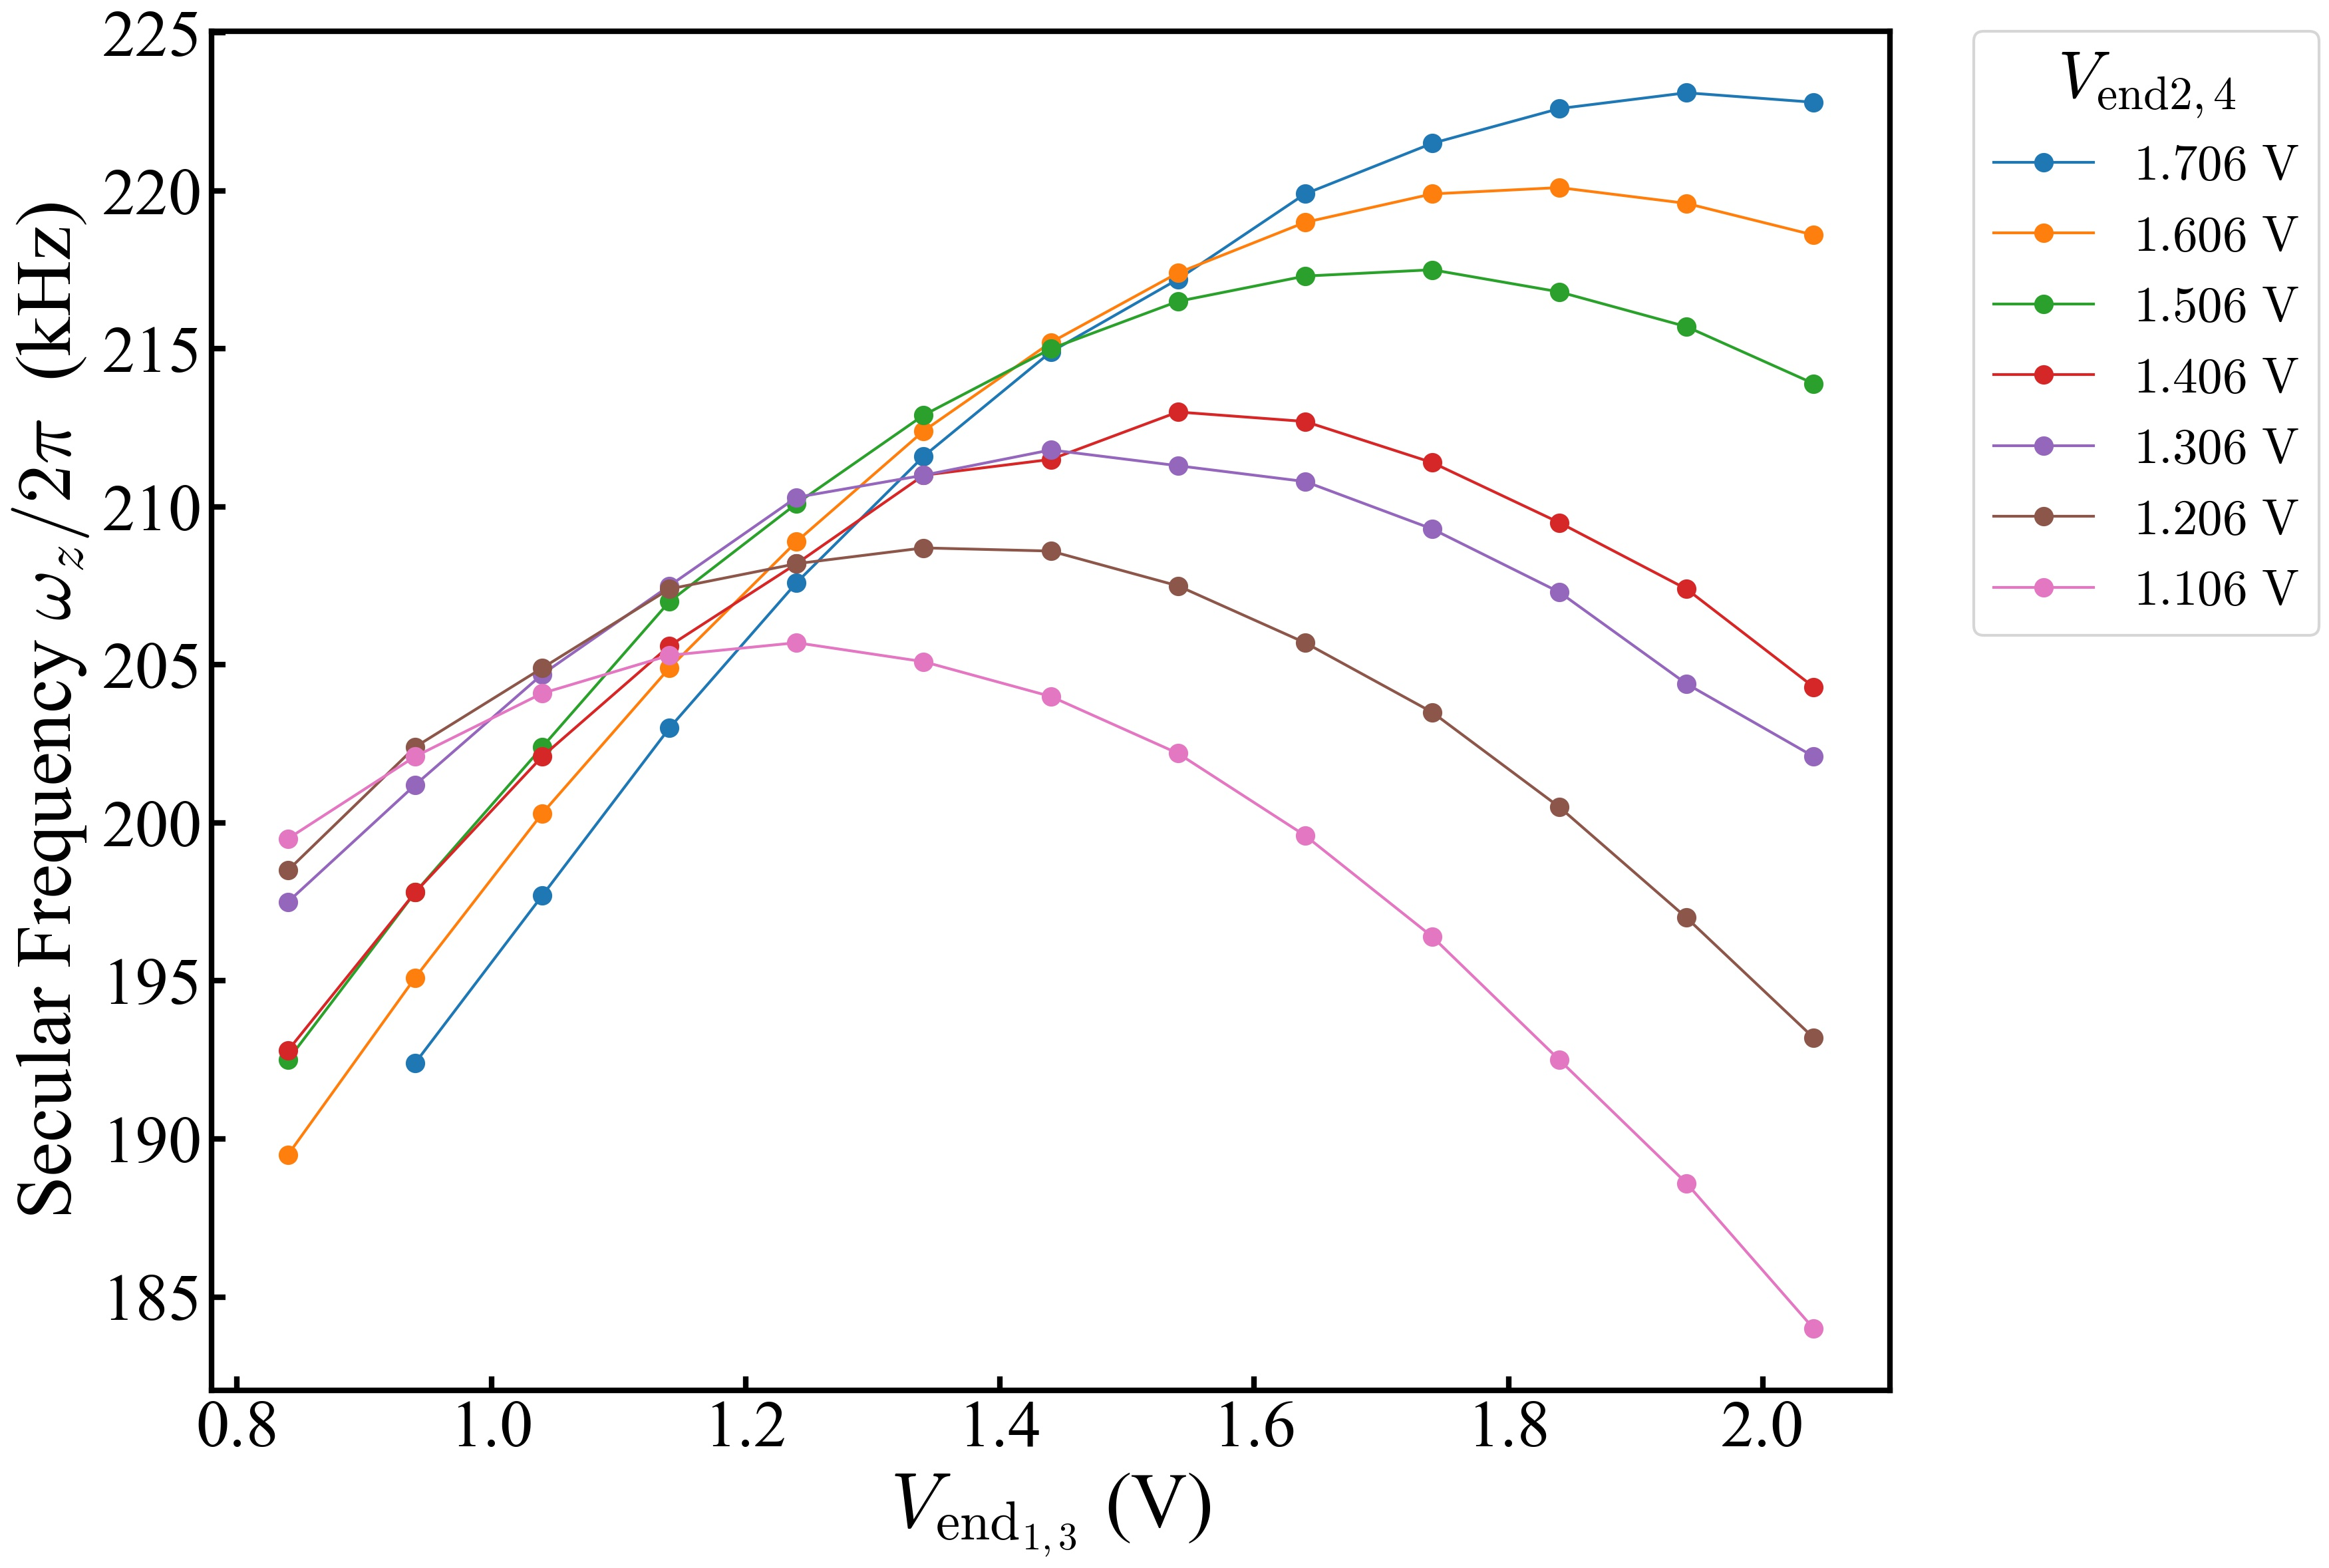
\includegraphics[width = 0.98\columnwidth]{./results/figure/Vendodd-SecFreqZ_Vendeven.jpg}
			\caption{\Fig{end13_MeasSec}と\Fig{end24_MeasSec}から得られた永年周波数の実験値}
			\label{fig:Vendodd_Vendeven}
		\end{center}
	\end{minipage}
	\begin{minipage}{0.5\linewidth}
		\begin{center}
			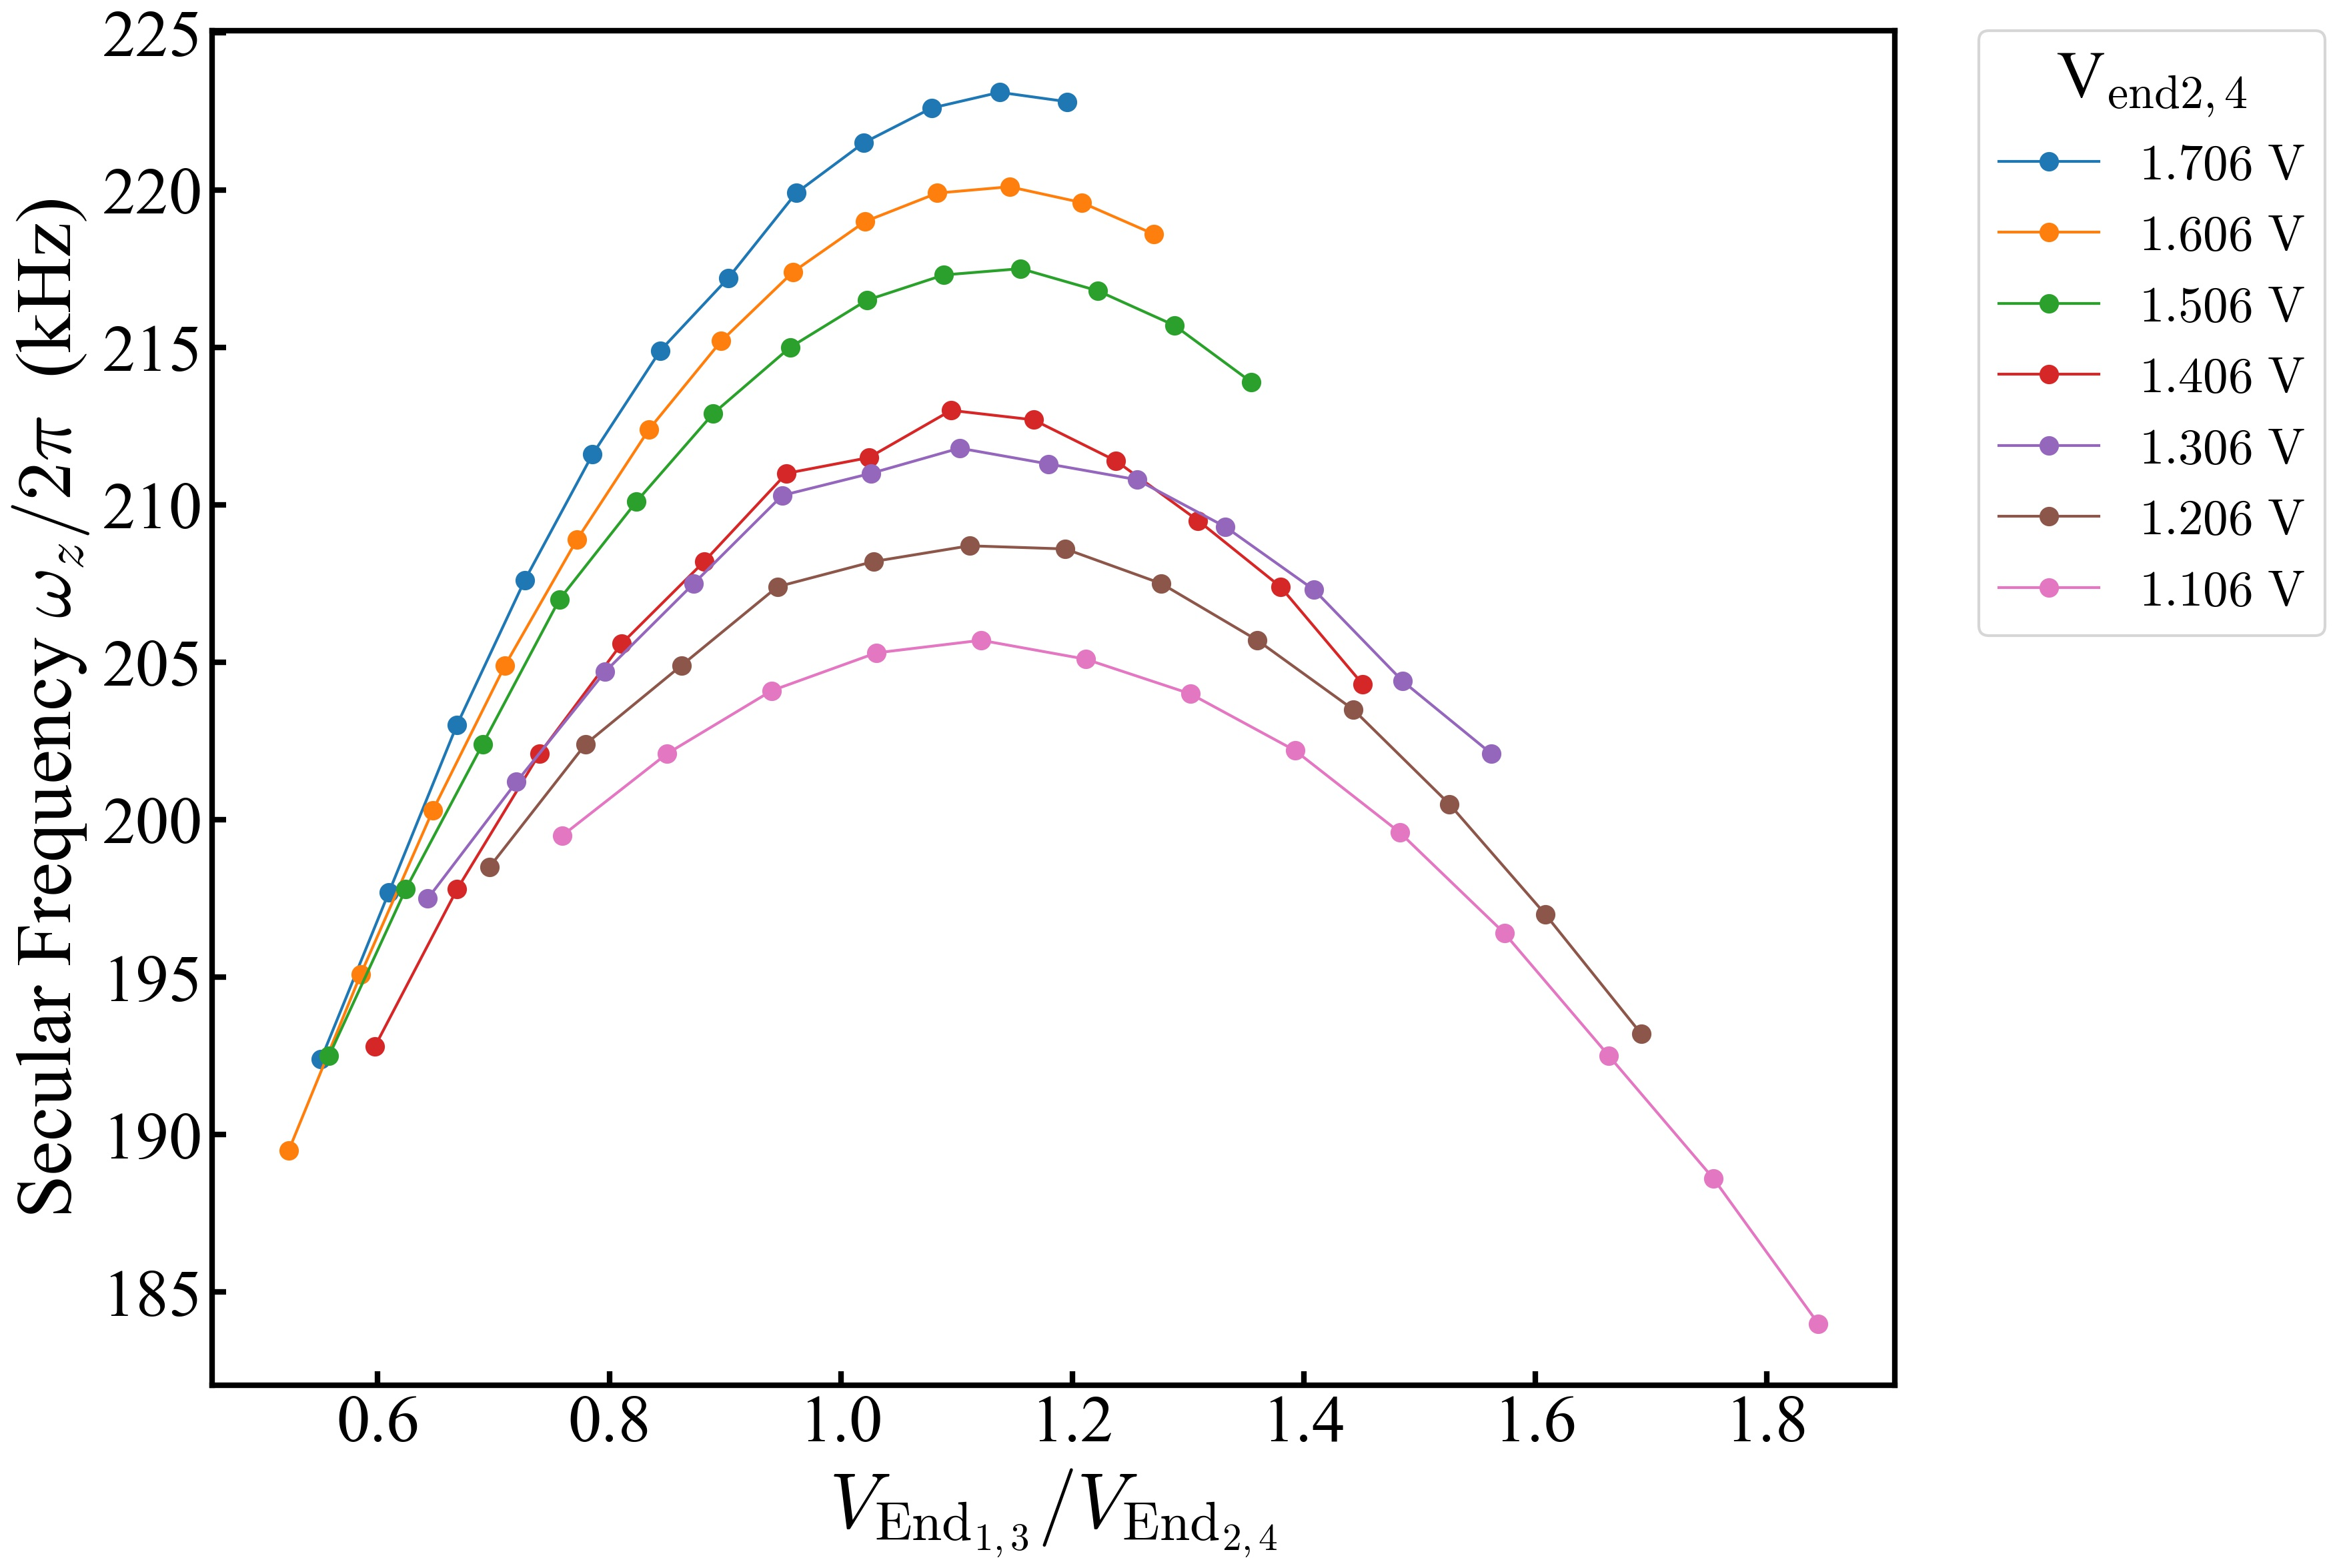
\includegraphics[width = 0.98\columnwidth]{./results/figure/Vendodd_Vendeven-SecFreqZ_.jpg}
			\caption{\Fig{Vendodd_Vendeven}より,永年周波数のf特性}
			\label{fig:Vendodd_Vendeven_f}
		\end{center}
	\end{minipage}
\end{figure}

さらに,$V_{\rm End2,4}$の各電圧値に対する永年周波数の$V_{\rm End1,3}$特性の変化率の比較を行うため,各$V_{\rm End1,3}$特性に対して永年周波数の規格化を行った.その結果を\Fig{Norm_Vendodd_Vendeven_f}に示す.

\begin{figure}[h]
	\begin{center}
		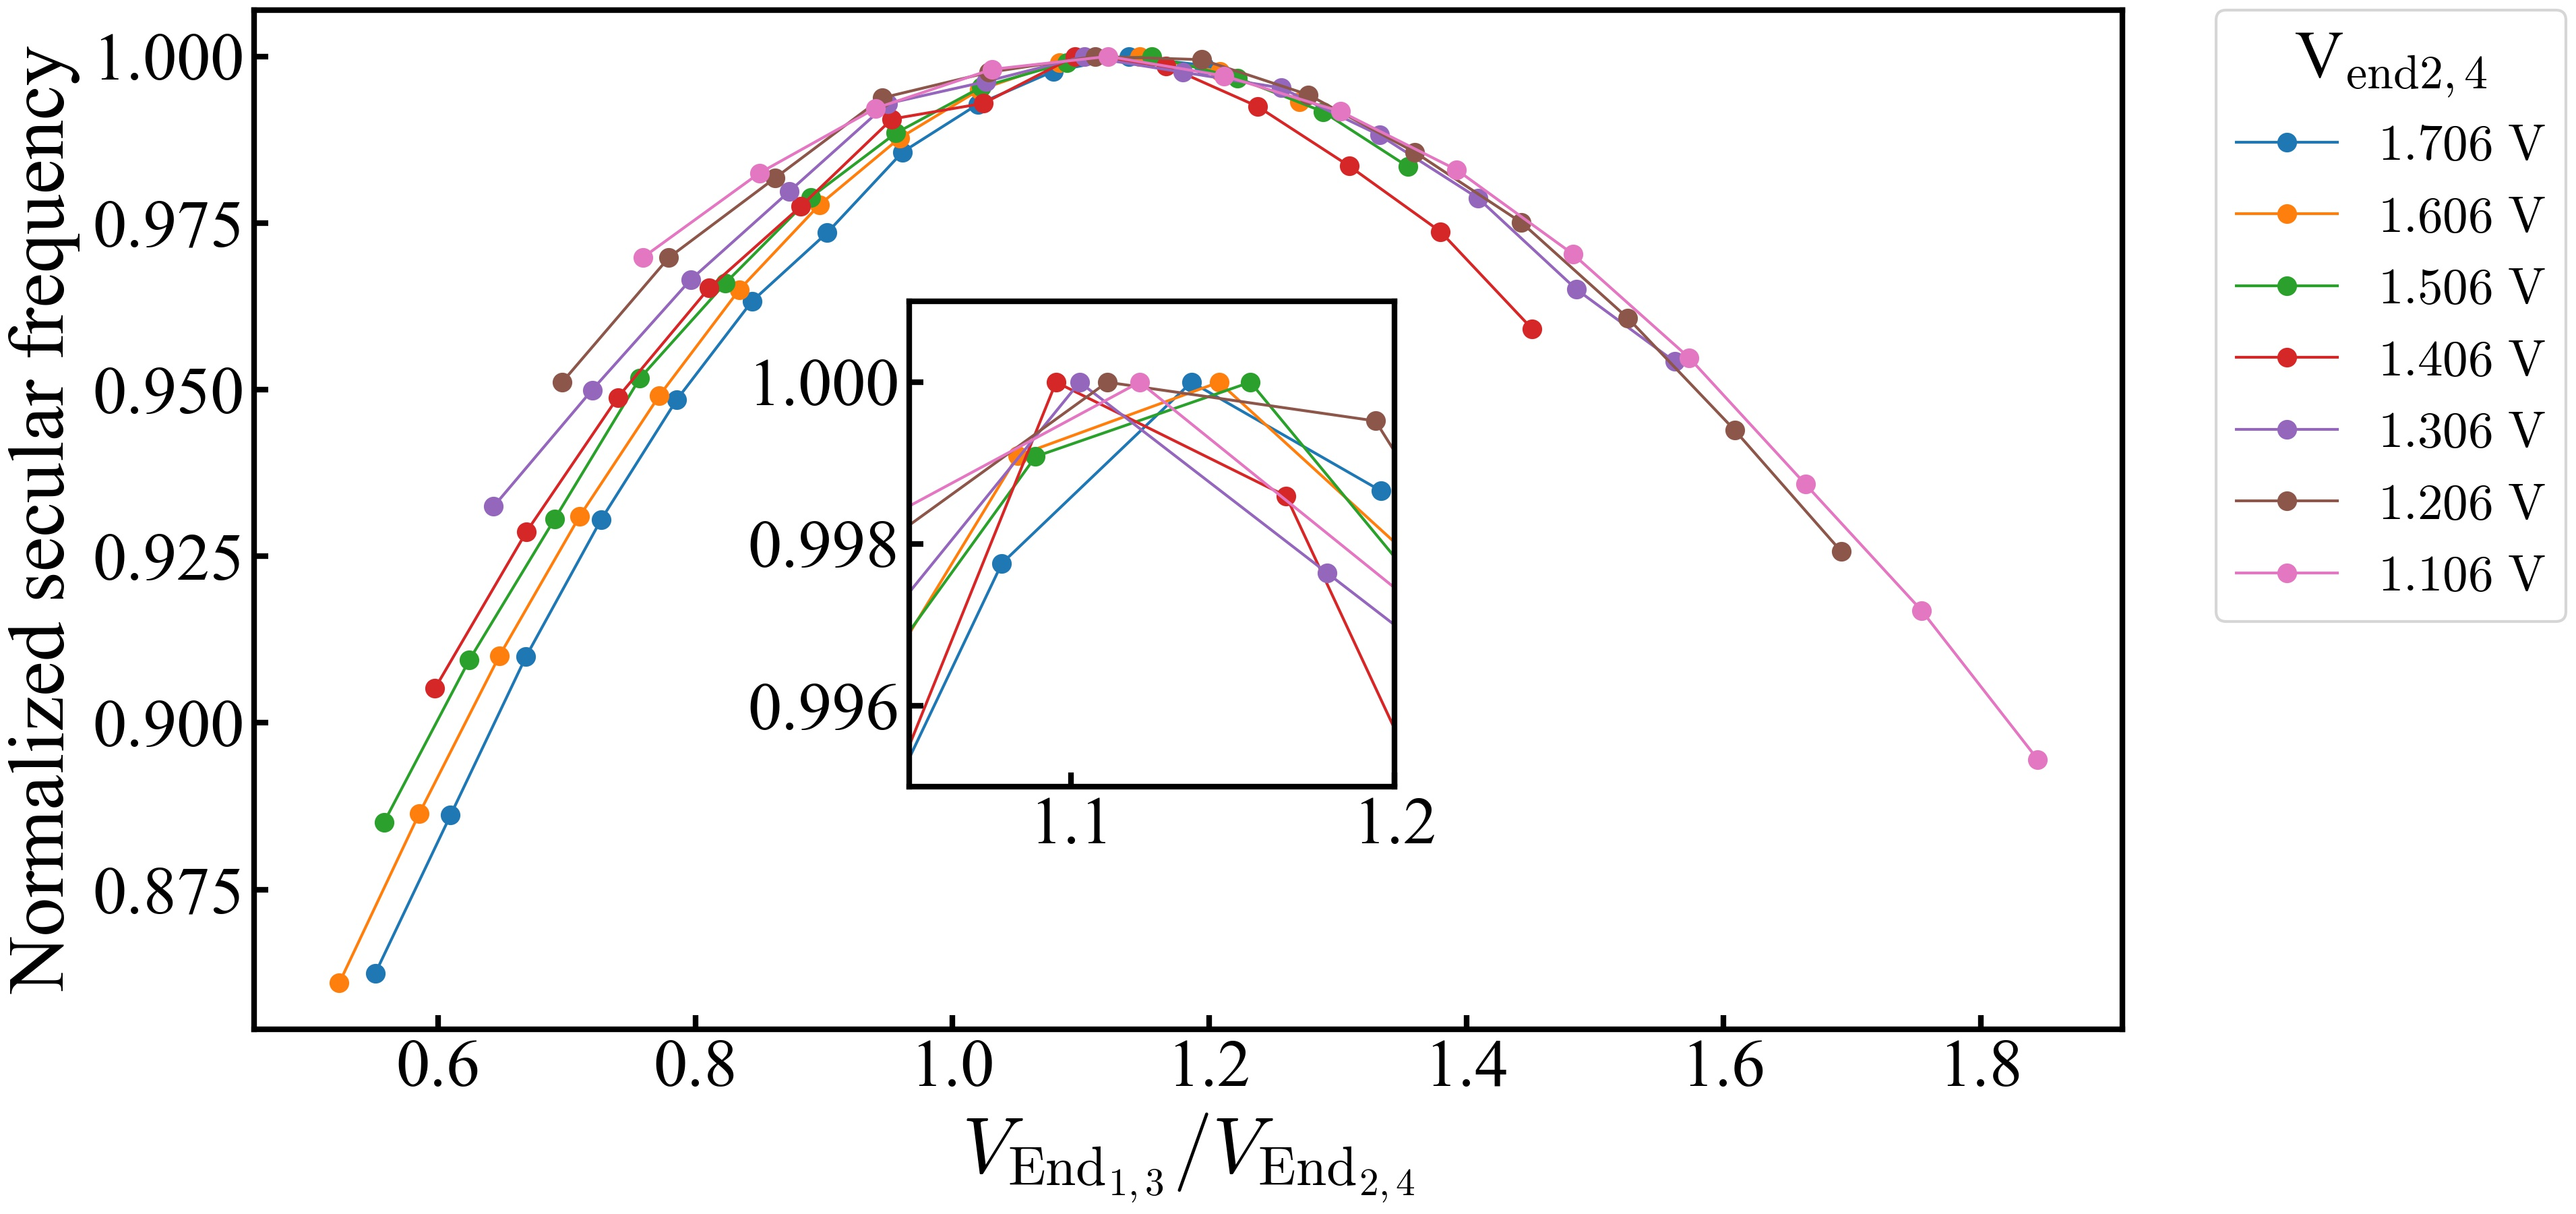
\includegraphics[width = 0.7\linewidth]{./results/figure/Normalized_Vendodd_Vendeven-SecFreqZ_.jpg}
		\caption{\Fig{Vendodd_Vendeven_f}において,$V_{\rm End2,4}$のそれぞれの条件における永年周波数で規格化した場合の永年周波数のf特性}
		\label{fig:Norm_Vendodd_Vendeven_f}
	\end{center}
\end{figure}

\Fig{Norm_Vendodd_Vendeven_f}より,$f \ \simeq \ 1.1$で極値を取ることが分かった.これは電極が小型であるために,End1,End3電極とEnd2, End4電極のそれぞれの電極形状の差が原因であると考えられる.

\clearpage

最後に,$V_{\rm middle1}, \ V_{\rm middle2}$を変化させた場合のイオンの振幅の周波数特性を\Fig{mid_MeasSec}に示す.

\begin{figure}[h]
	\begin{center}
		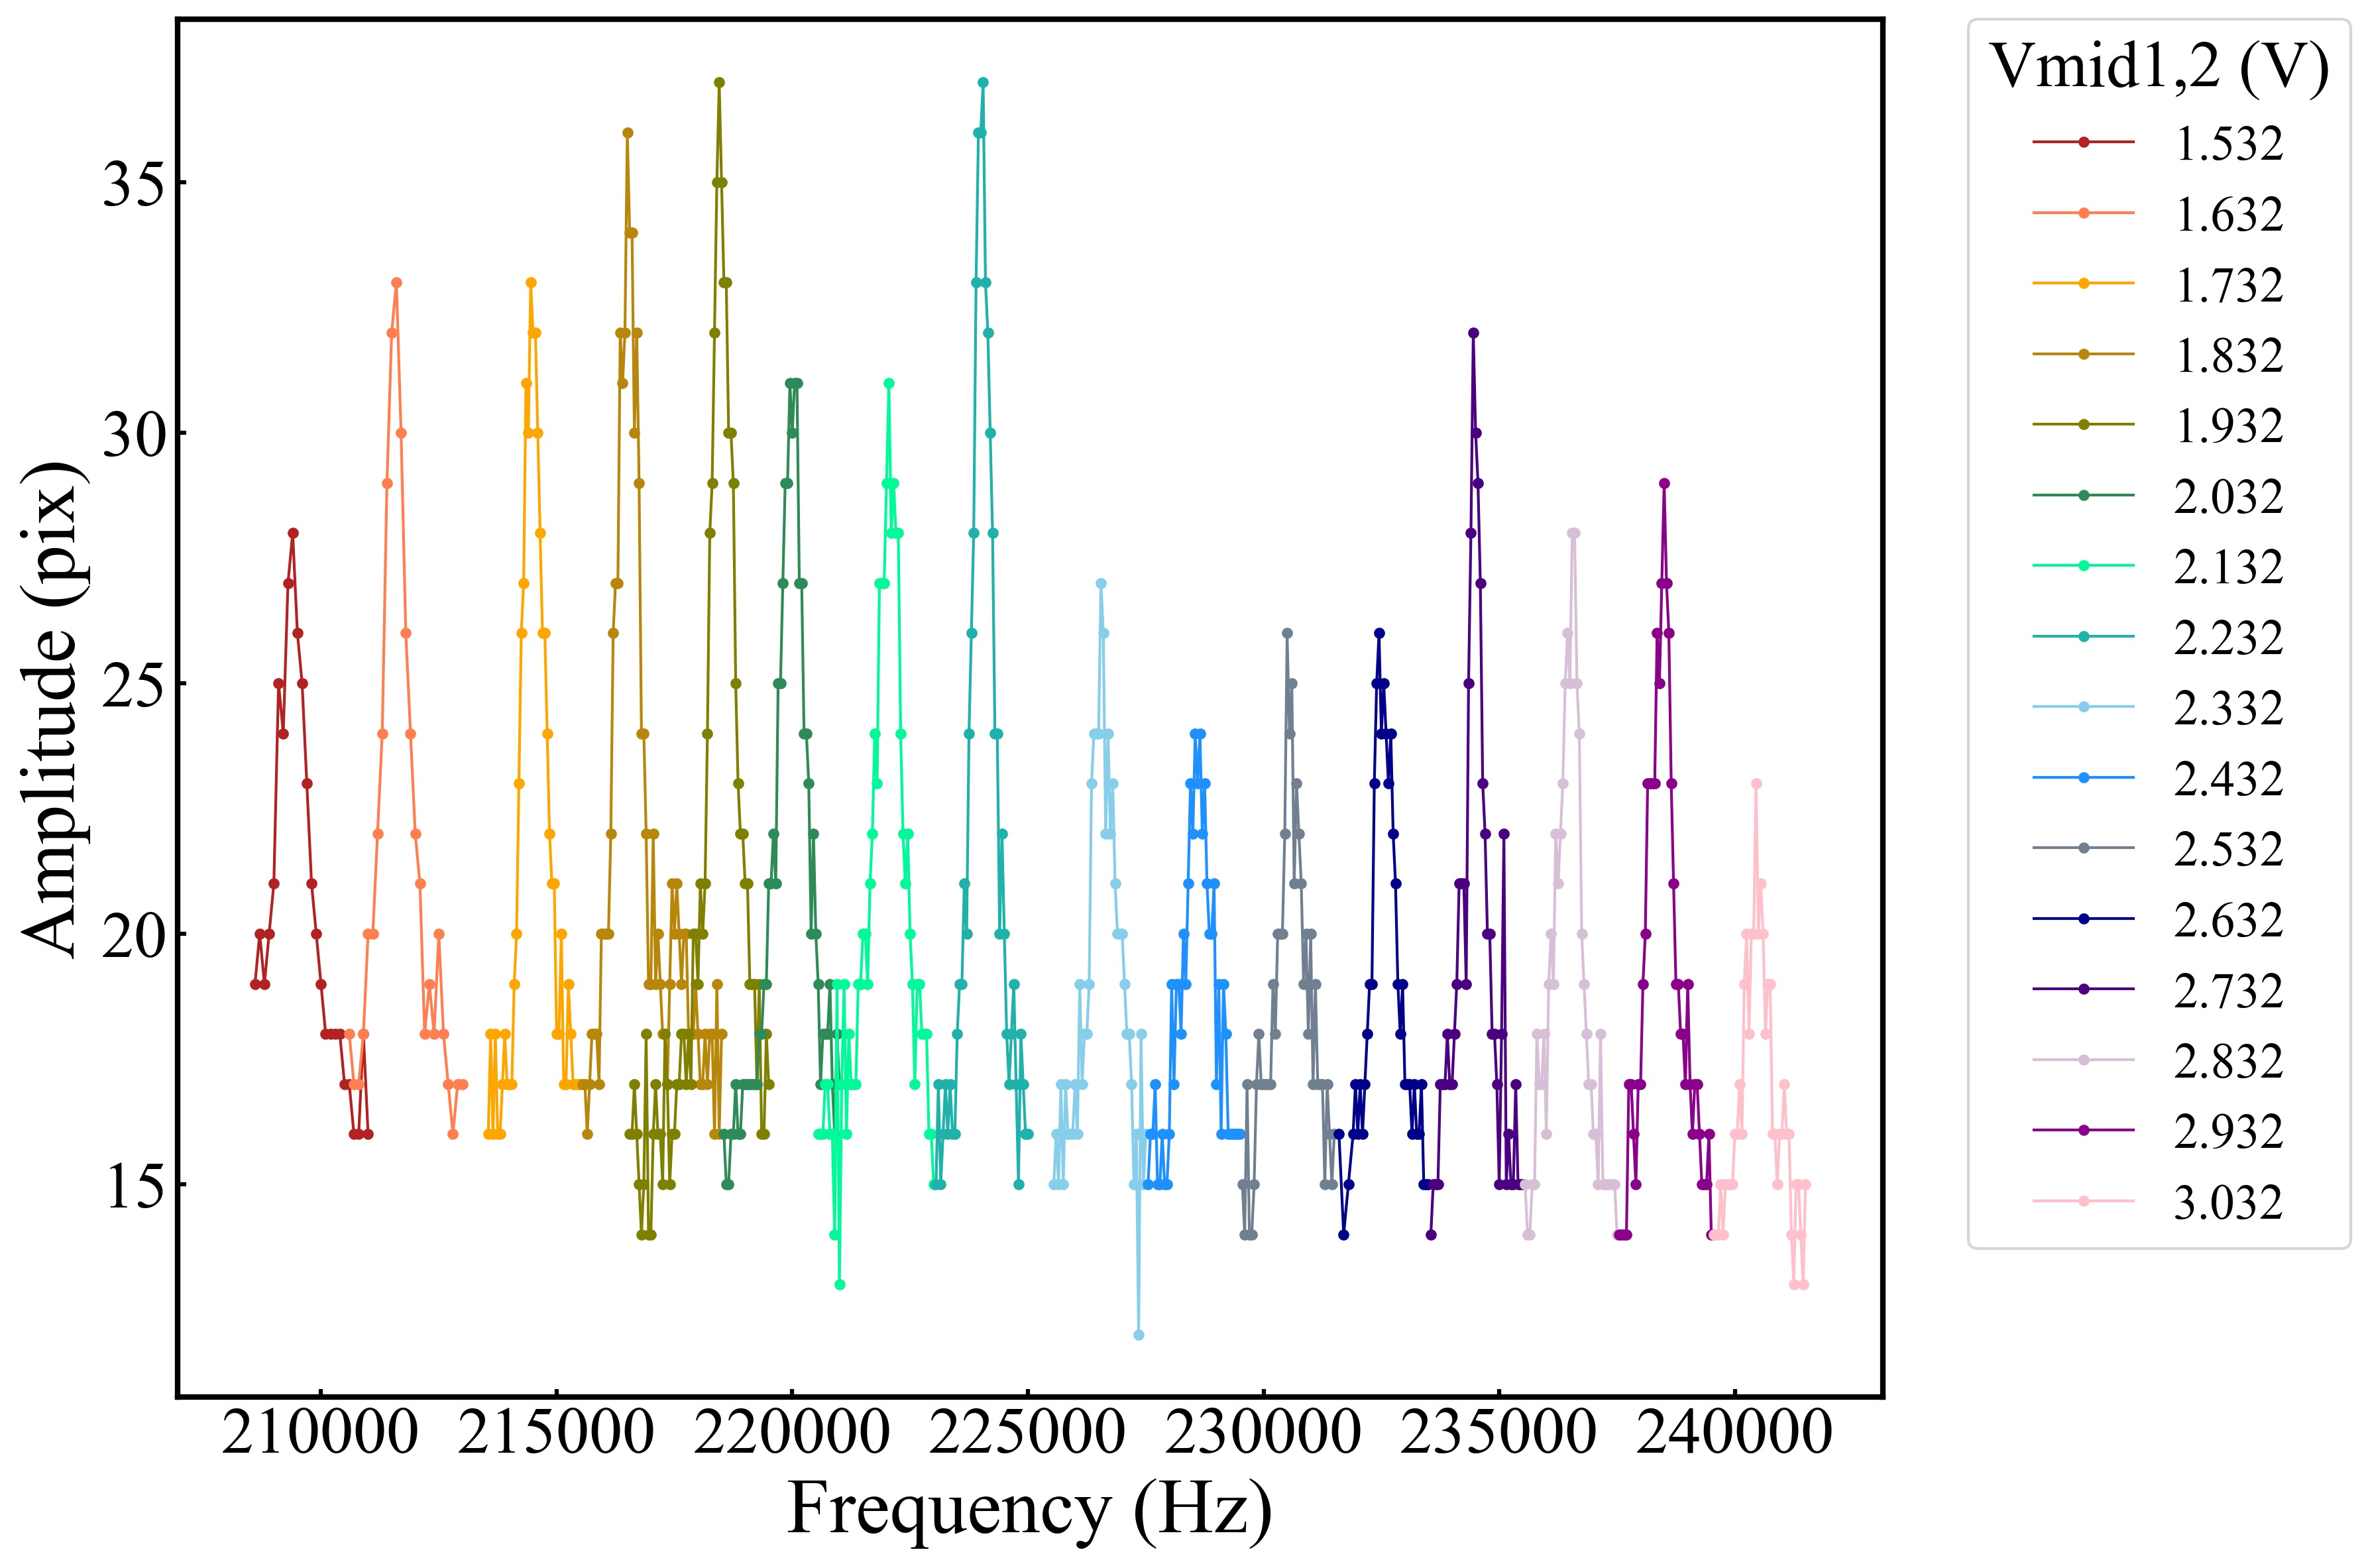
\includegraphics[width = 0.6\linewidth]{./results/figure/mid-SecFreq.jpg}
		\caption{$V_{\rm middle1}$と$V_{\rm middle2}$を変化させたときのイオンの振幅の周波数特性}
		\label{fig:mid_MeasSec}
	\end{center}
\end{figure}

\Fig{mid_MeasSec}からローレンツ分布関数によるフィッティングによって得られる永年周波数とシミュレーションから得られる永年周波数との比較を\Fig{mid12_MeasSec_SimSec}に示す.

\begin{figure}[h]
	\begin{center}
		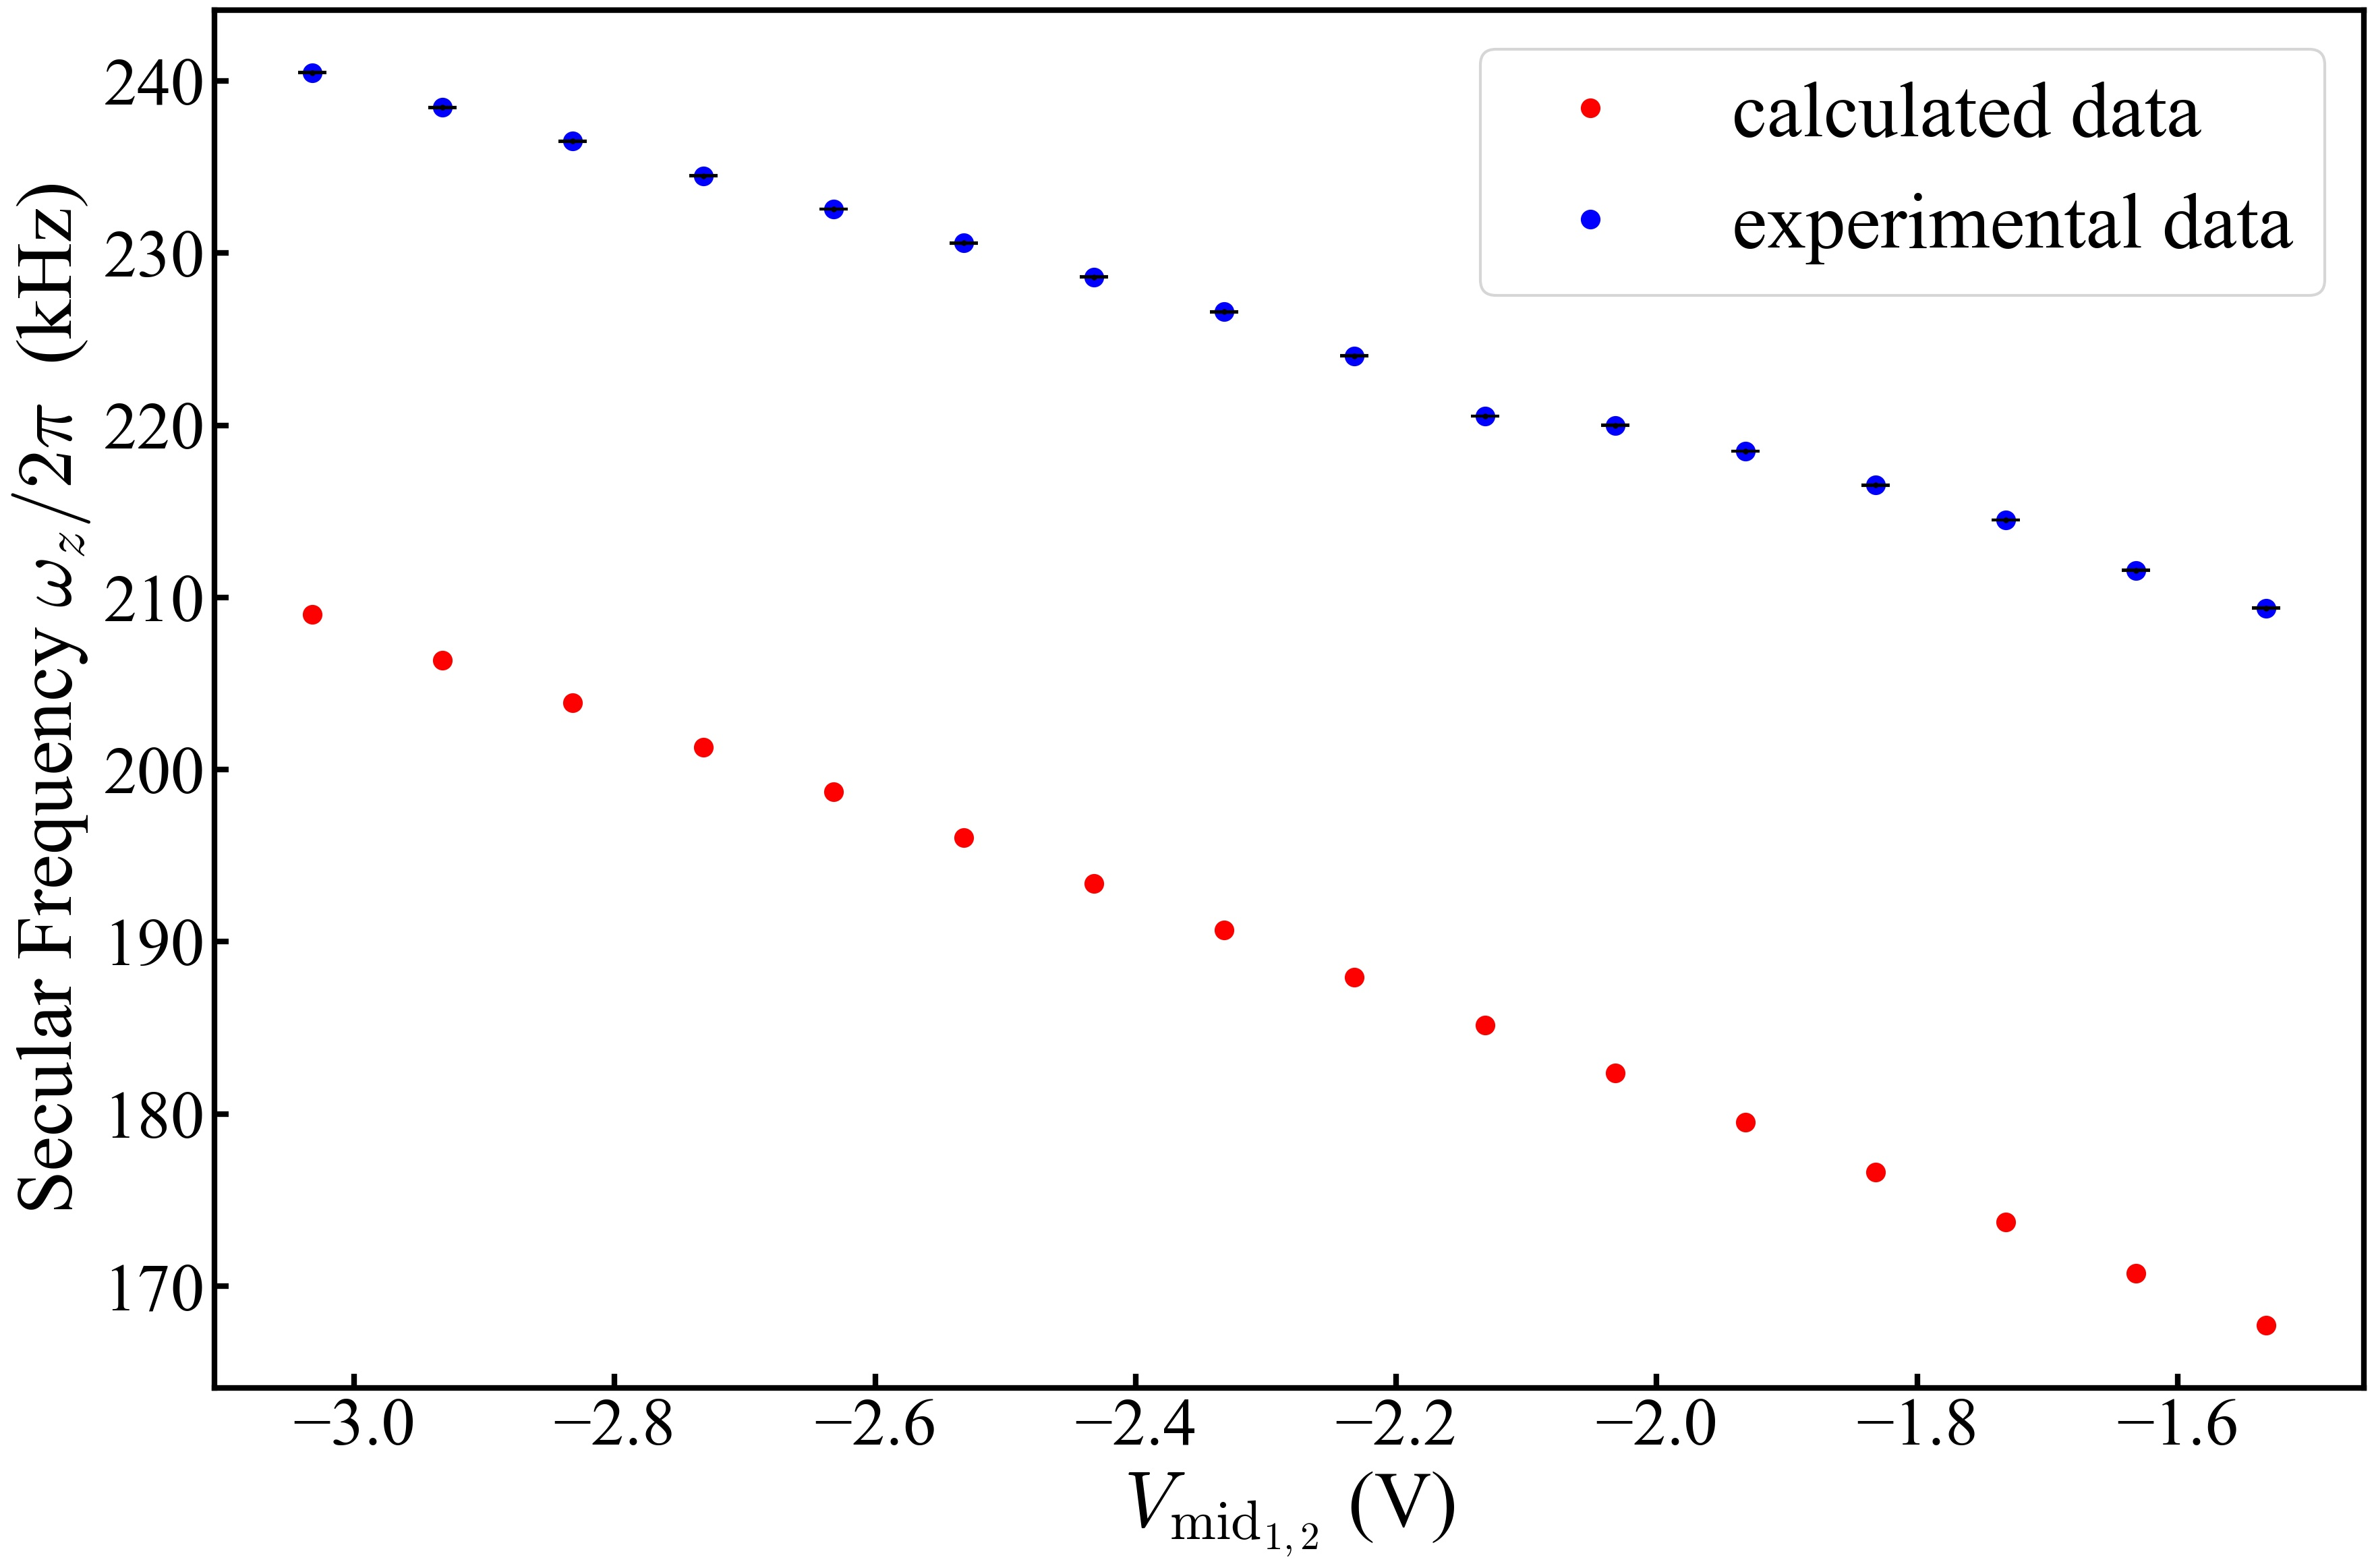
\includegraphics[width = 0.6\linewidth]{./results/figure/Vmid-SecFreqZ.jpg}
		\caption{$V_{\rm middle1}$と$V_{\rm middle2}$を変化させたときの永年周波数の測定結果とシミュレーション結果との比較}
		\label{fig:mid12_MeasSec_SimSec}
	\end{center}
\end{figure}

\Fig{mid12_MeasSec_SimSec}から,実験値とシミュレーション値に$33.2 \ {\rm kHz} \ \sim \ 41.7 \ {\rm kHz}$の差が存在することが分かった.

[挿入予定]永年周波数のrf振幅特性 \\
rf振幅を変化させたときの永年周波数の変化がdc電圧を変化させたときと比較して小さいので,無視する.したがって,rf擬ポテンシャルによって永年周波数の実験値とシミュレーション値との差が生まれているとは考えない.

\clearpage

\subsection{永年周波数の測定結果から導く電場の傾き}

\subsection{イオン捕獲位置特定による電場検出結果}
プレーナートラップ上に形成される電場$\bm{E}$から受ける力と,複数個イオン($N \ geq$ 2)で生じるクーロン相互作用がつり合う位置がイオンの平衡位置となる.$N \ = \ 2 \ \sim \ 6$個のイオンを用いて,それぞれのイオン捕獲位置における電場の算出を\Eq{equi_string}を用いて行った.このとき,単一イオンを捕獲したときの位置を中心に取っている.なお,実験は\Tb{dc_string}の条件に対して,$V_{rm  1,3} \ = 1.24 \ {\rm V} \ ({\rm DC1})$,$V_{\rm End 1,3} \ = 1.44 \ {\rm V} \ ({\rm DC2})$,$V_{\rm End 1,3} \ = 1.64 \ {\rm V} \ ({\rm DC3})$の3種類のdc電圧セットに対して行った.まず,DC1の条件で算出した電場の結果を示す.\Fig{DC1_N1} $\sim$ \Fig{DC1_N6}に$N \ = \ 1 \ \sim \ 6$個のイオンを捕獲したときのイオン捕獲位置での電場の算出結果を示す.

\begin{figure}[h]
	\begin{minipage}{0.33\linewidth}
		\begin{center}
			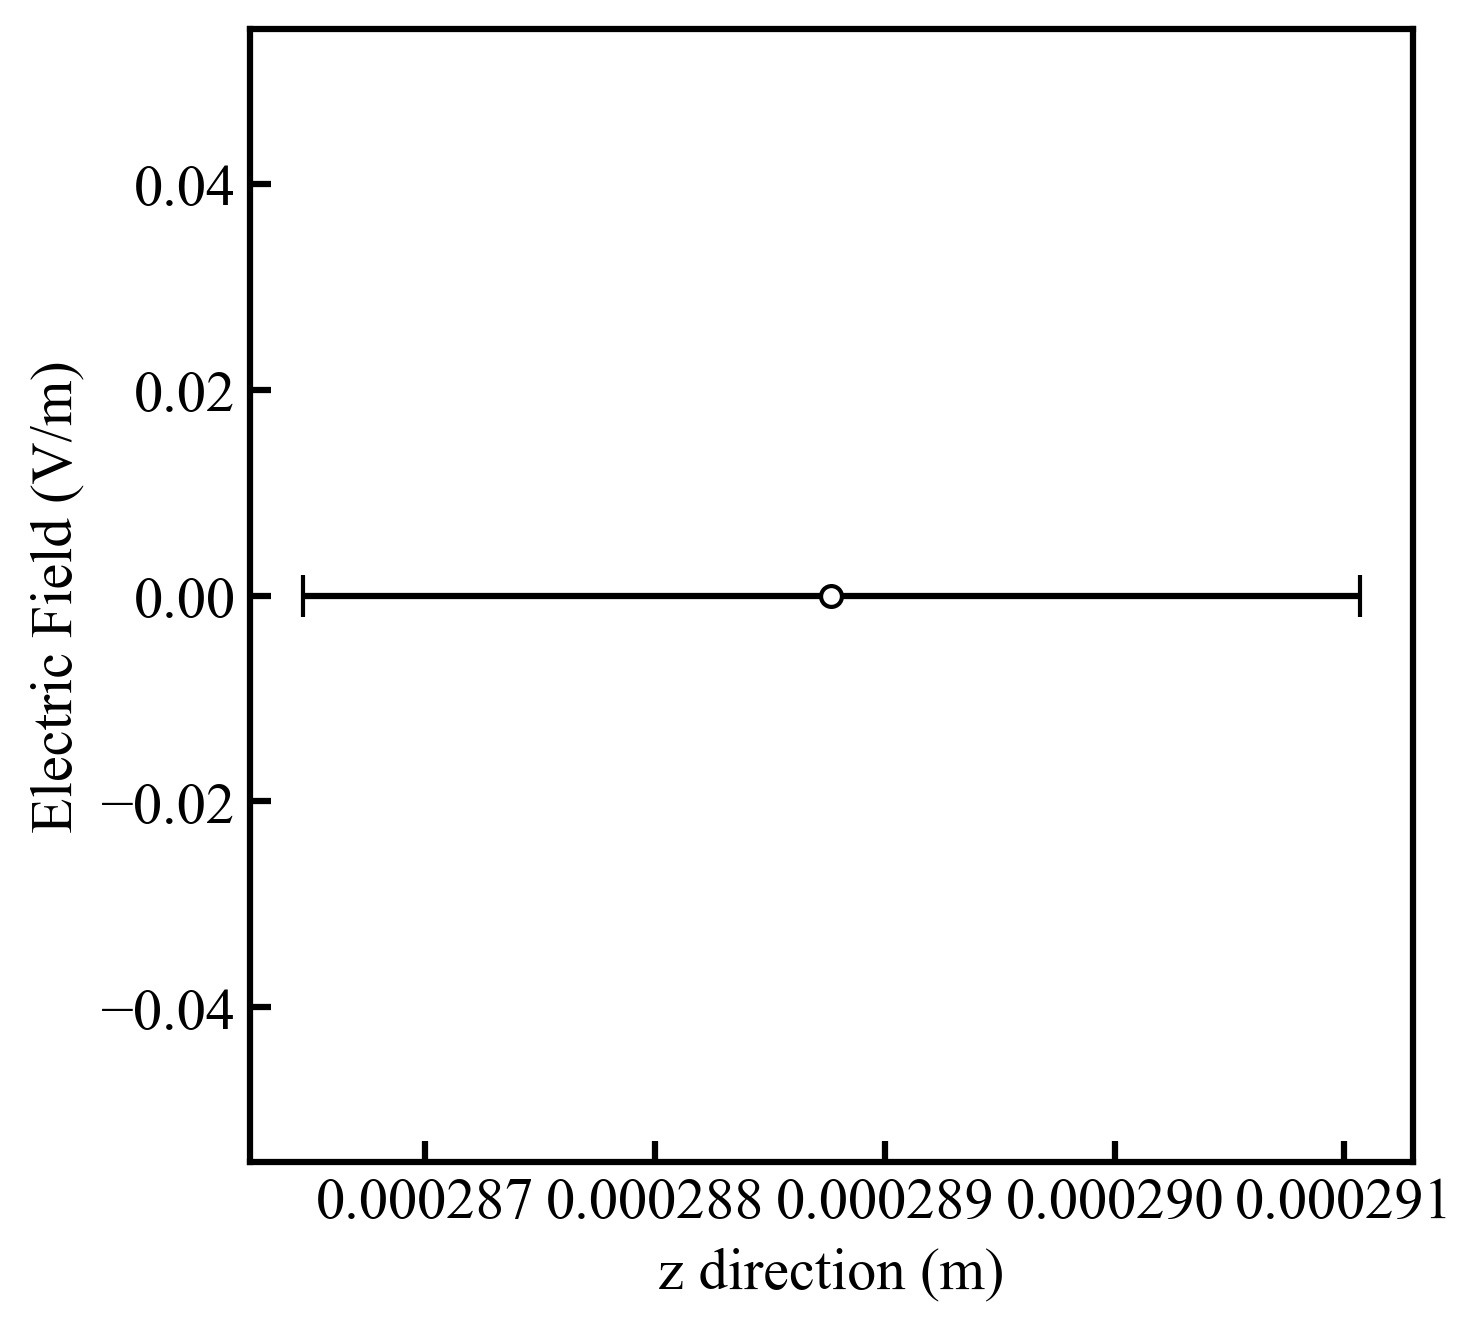
\includegraphics[width = 0.9\columnwidth]{./results/figure/DC1_N1.jpg}
			\caption{dc電圧セットDC1において$N=1$のときの電場算出結果}
			\label{fig:DC1_N1}
		\end{center}
	\end{minipage}
	\begin{minipage}{0.33\linewidth}
		\begin{center}
			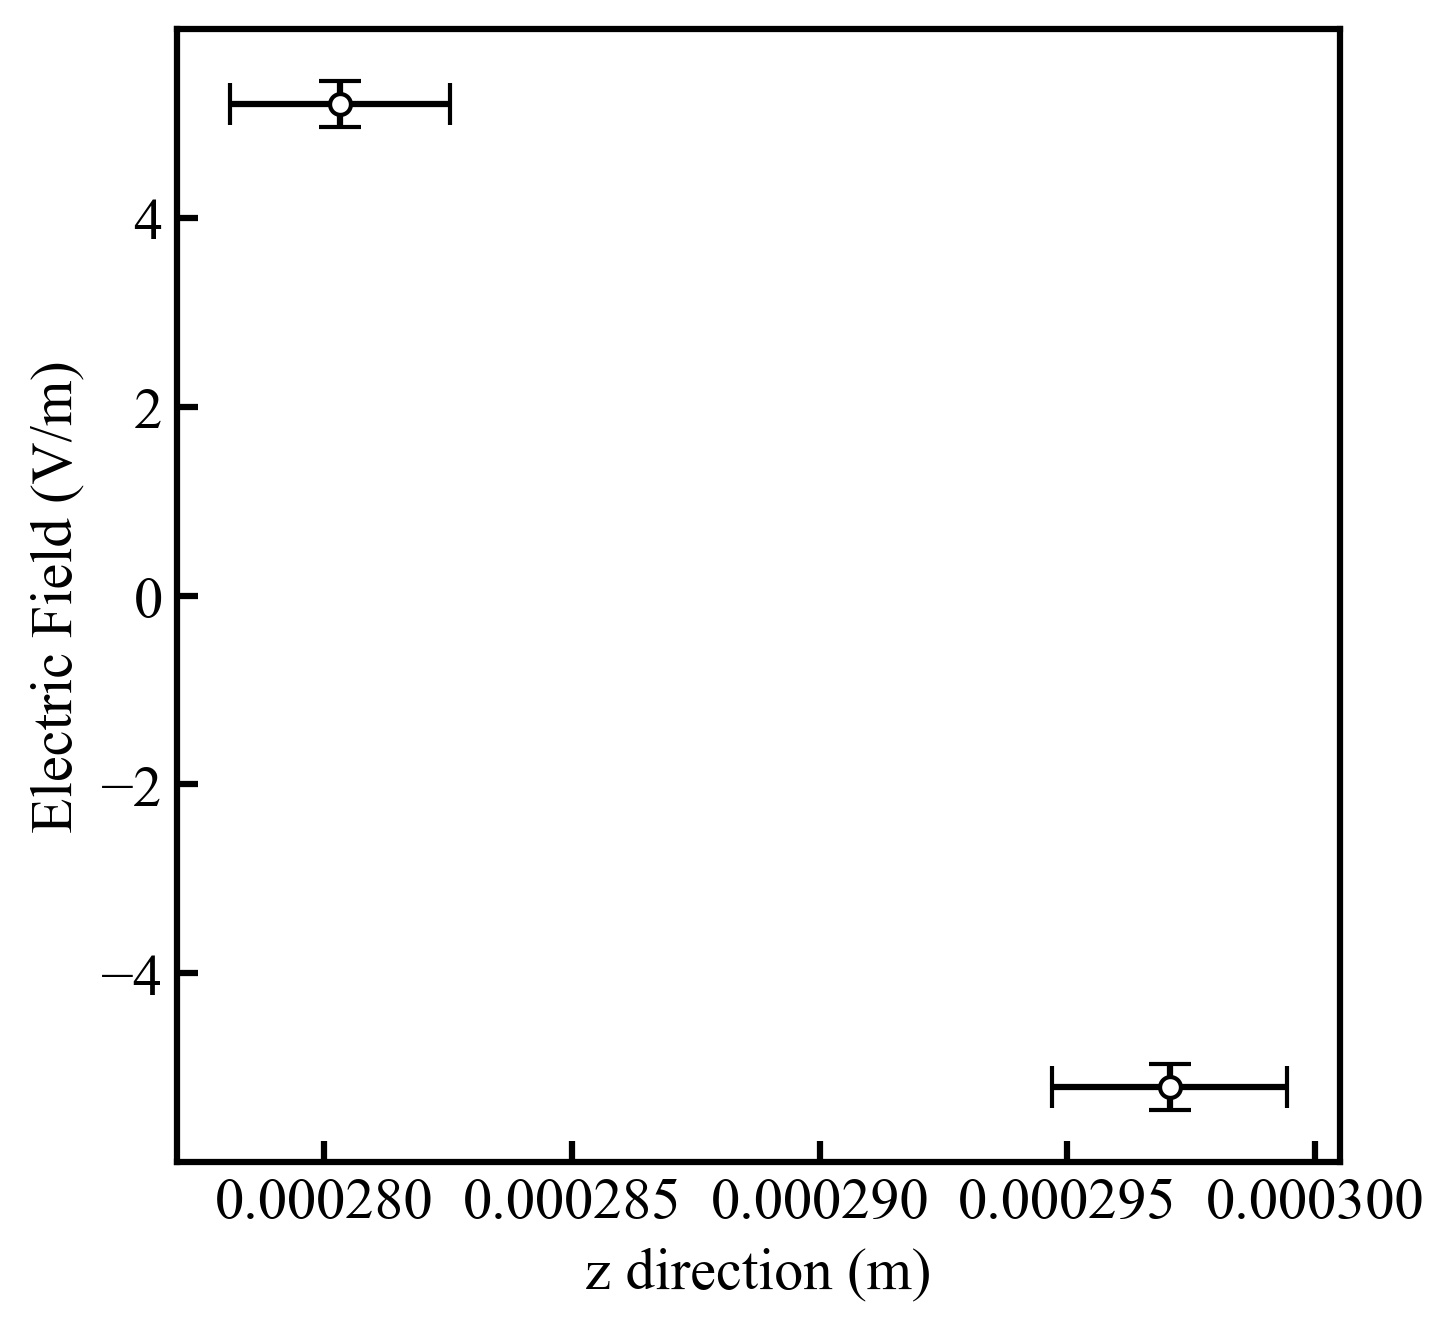
\includegraphics[width = 0.9\columnwidth]{./results/figure/DC1_N2.jpg}
			\caption{dc電圧セットDC1において$N=2$のときの電場算出結果}
			\label{fig:DC1_N2}
		\end{center}
	\end{minipage}
	\begin{minipage}{0.33\linewidth}
		\begin{center}
			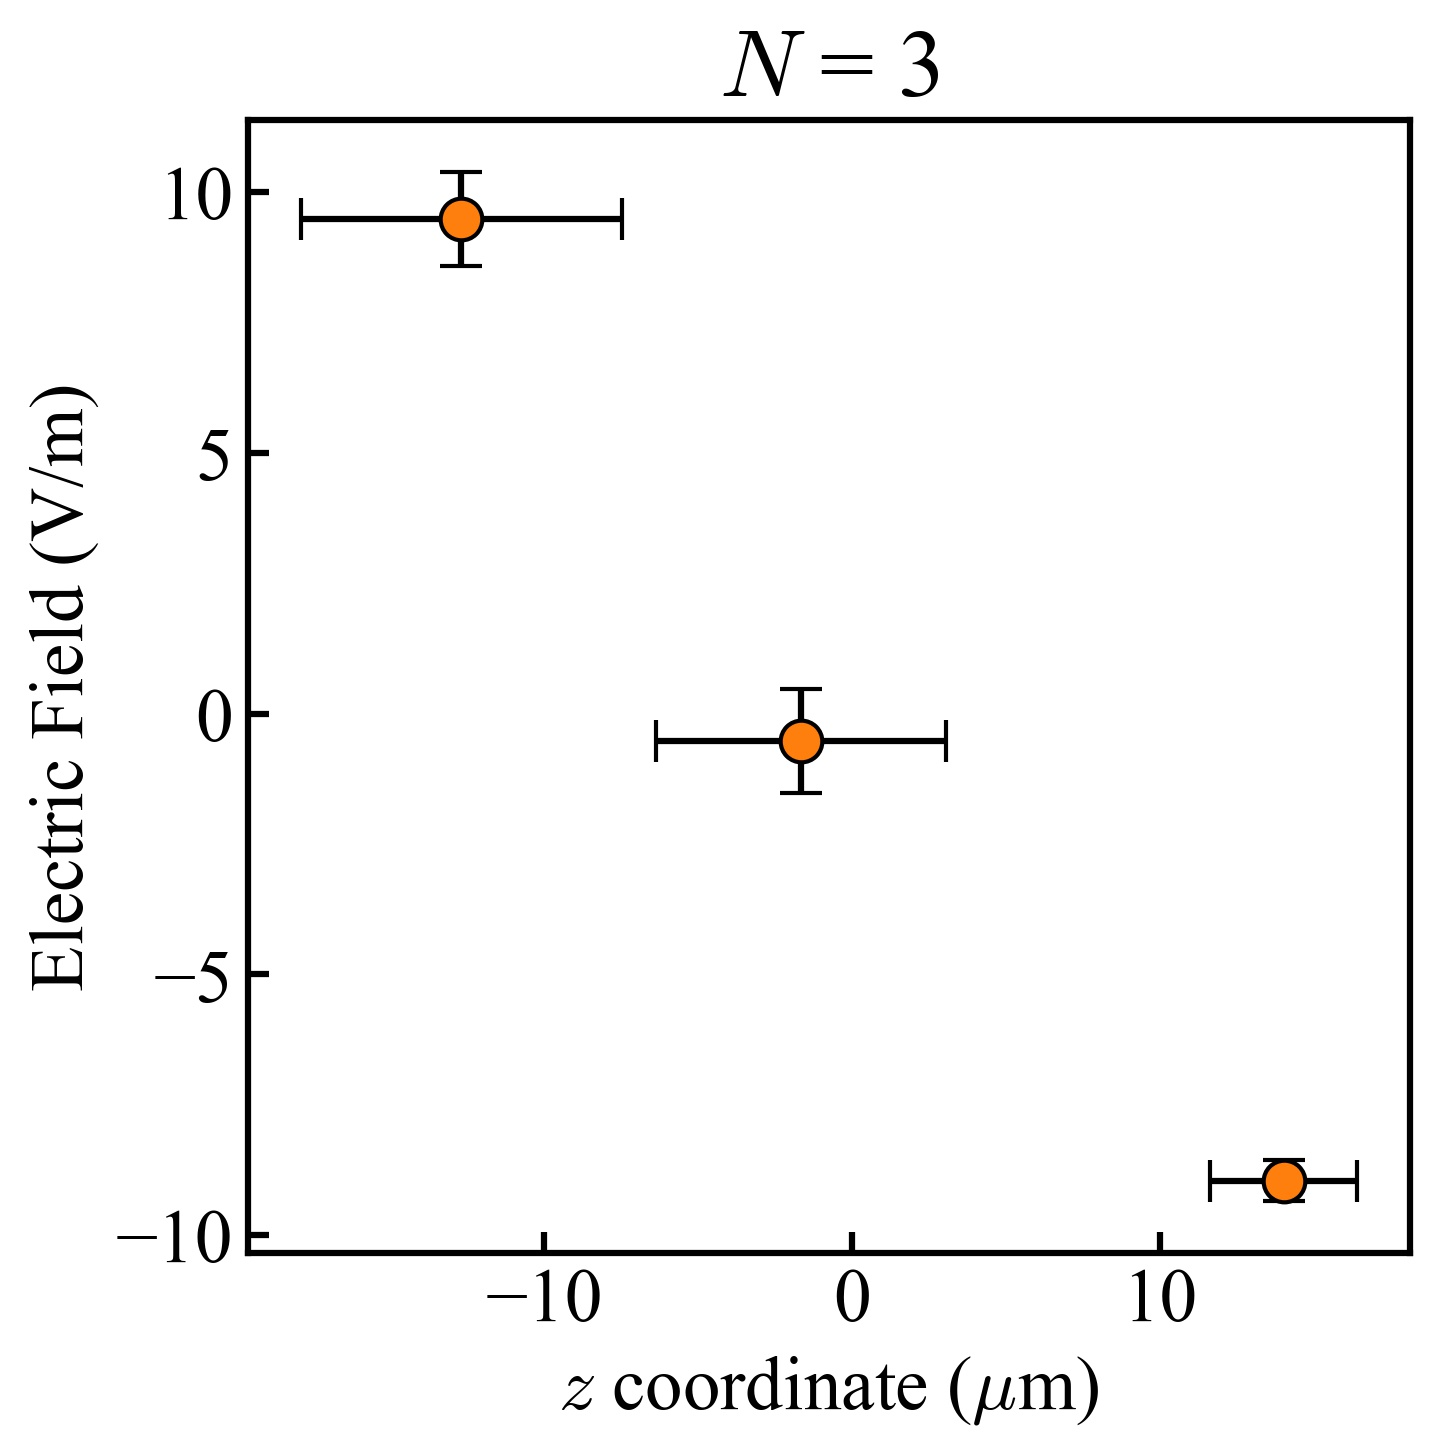
\includegraphics[width = 0.9\columnwidth]{./results/figure/DC1_N3.jpg}
			\caption{dc電圧セットDC1において$N=3$のときの電場算出結果}
			\label{fig:DC1_N3}
		\end{center}
	\end{minipage}
\end{figure}

\begin{figure}[h]
	\begin{minipage}{0.33\linewidth}
		\begin{center}
			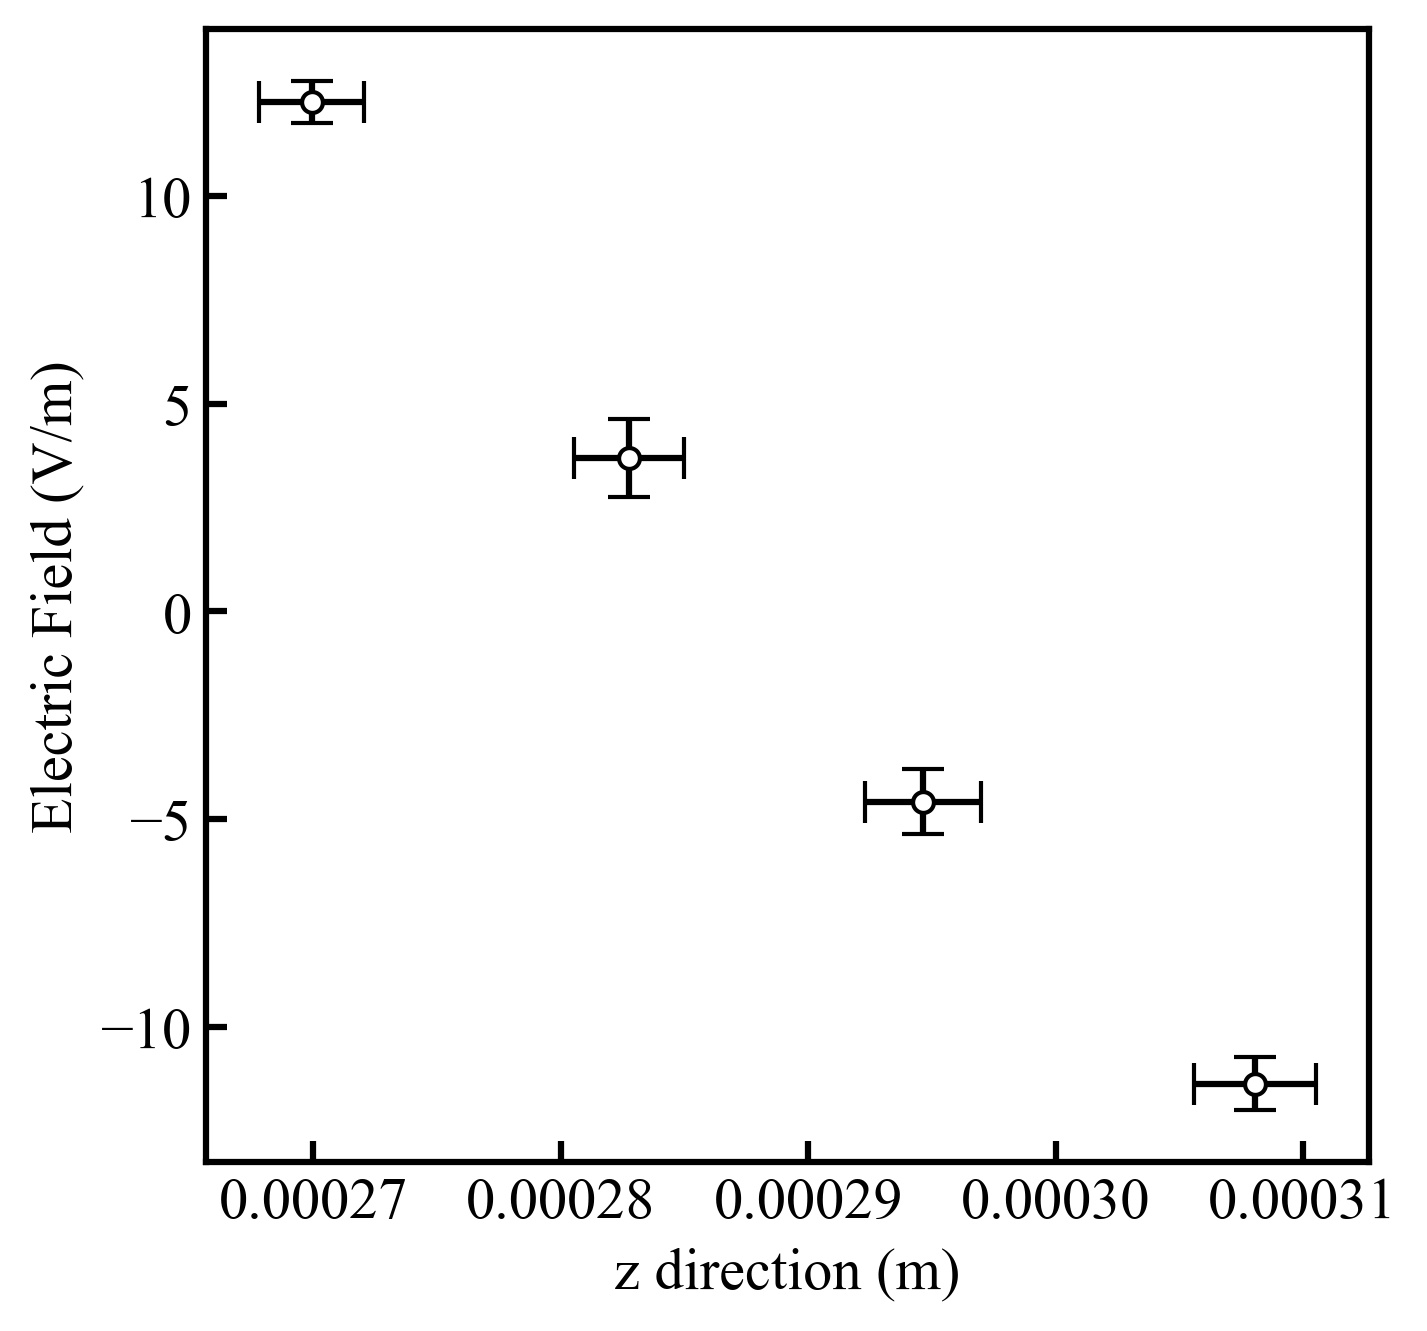
\includegraphics[width = 0.9\columnwidth]{./results/figure/DC1_N4.jpg}
			\caption{dc電圧セットDC1において$N=4$のときの電場算出結果}
			\label{fig:DC1_N4}
		\end{center}
	\end{minipage}
	\begin{minipage}{0.33\linewidth}
		\begin{center}
			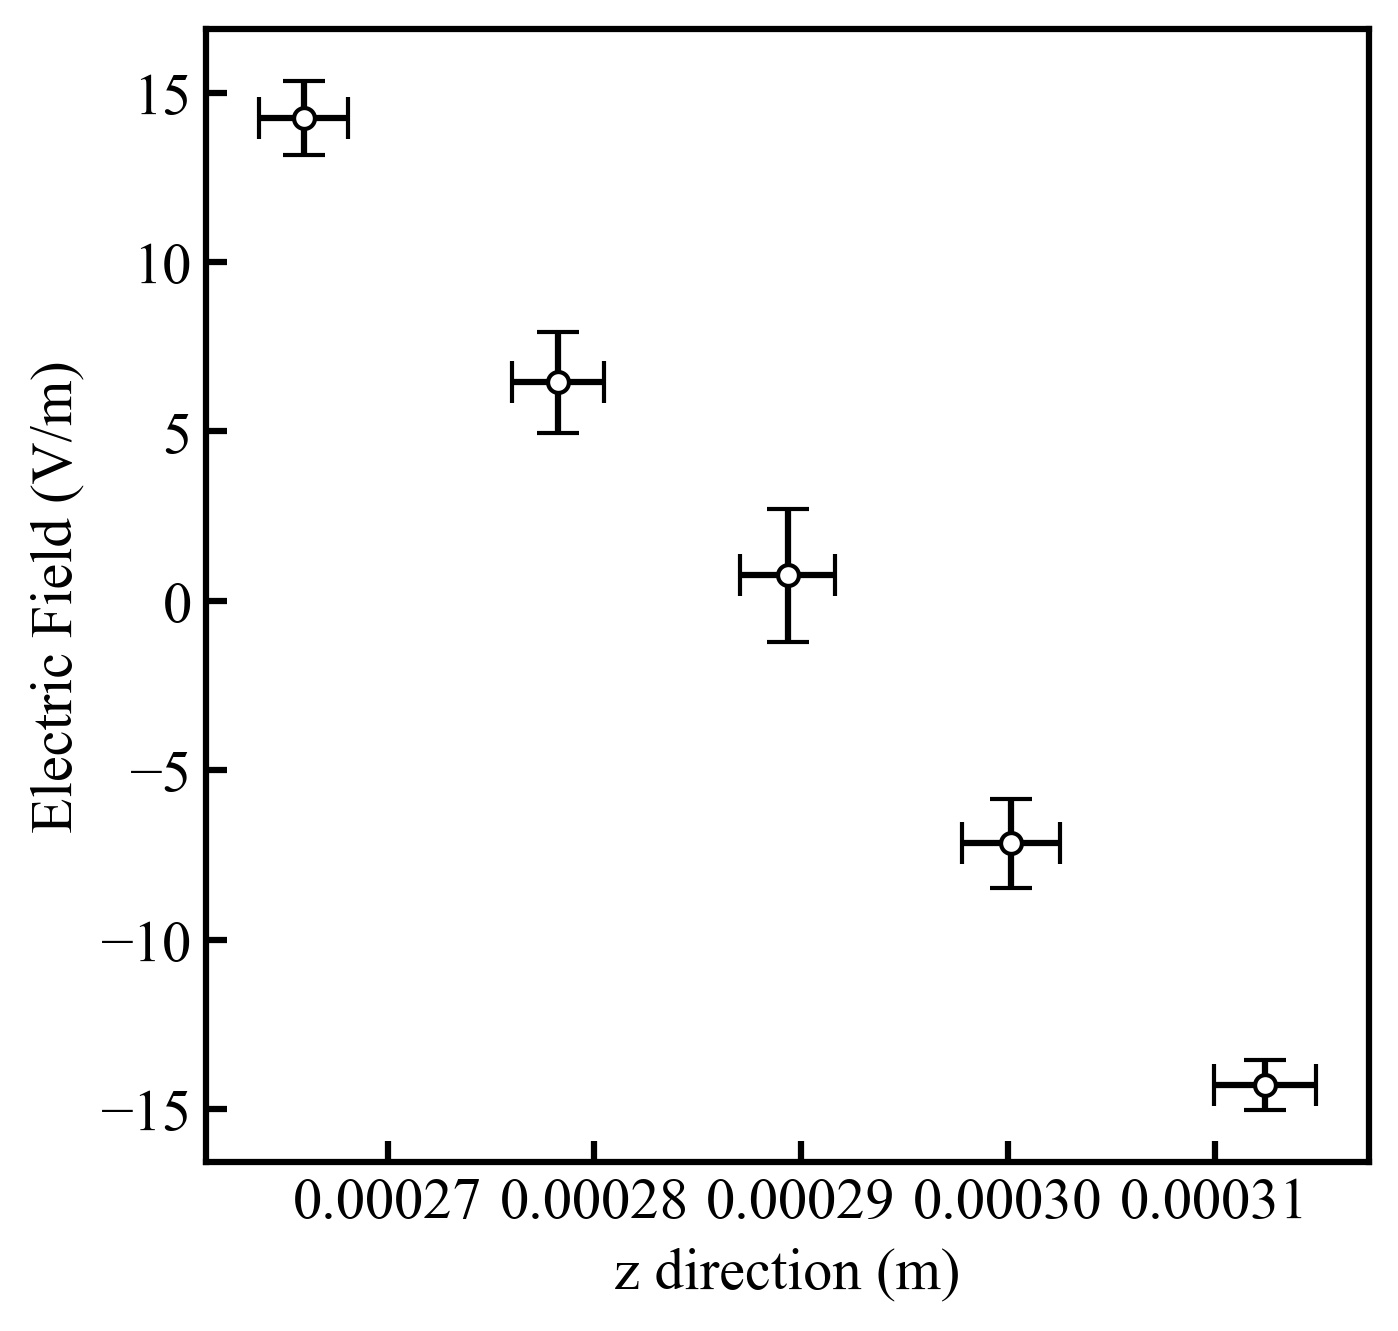
\includegraphics[width = 0.9\columnwidth]{./results/figure/DC1_N5.jpg}
			\caption{dc電圧セットDC1において$N=5$のときの電場算出結果}
			\label{fig:DC1_N5}
		\end{center}
	\end{minipage}
	\begin{minipage}{0.33\linewidth}
		\begin{center}
			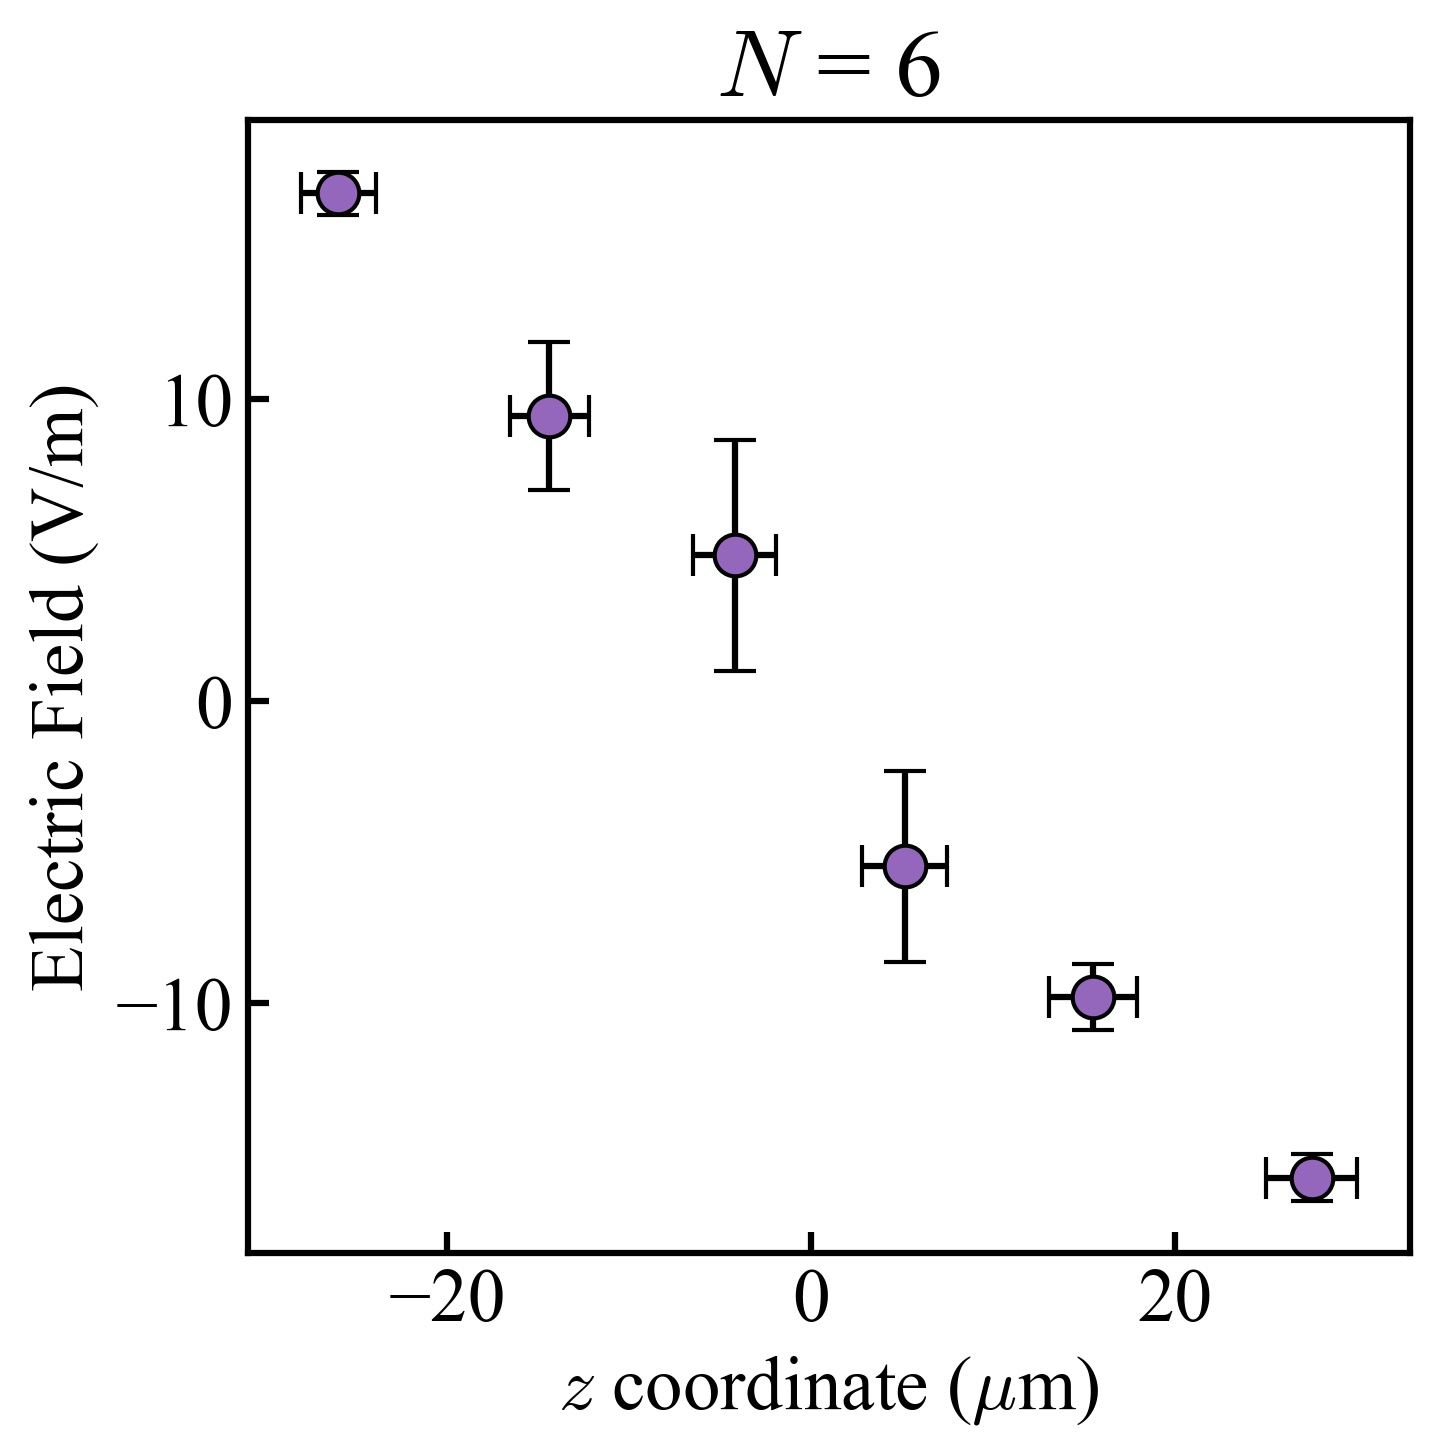
\includegraphics[width = 0.9\columnwidth]{./results/figure/DC1_N6.jpg}
			\caption{dc電圧セットDC1において$N=6$のときの電場算出結果}
			\label{fig:DC1_N6}
		\end{center}
	\end{minipage}
\end{figure}

\Fig{DC1_N1} $\sim$ \Fig{DC1_N6}から算出されたイオン捕獲位置における電場の値を同一のグラフにまとめ,一次関数によるフィッティングを行った.その結果を\Fig{DC1_E}に示す.

\begin{figure}[h]
	\begin{center}
		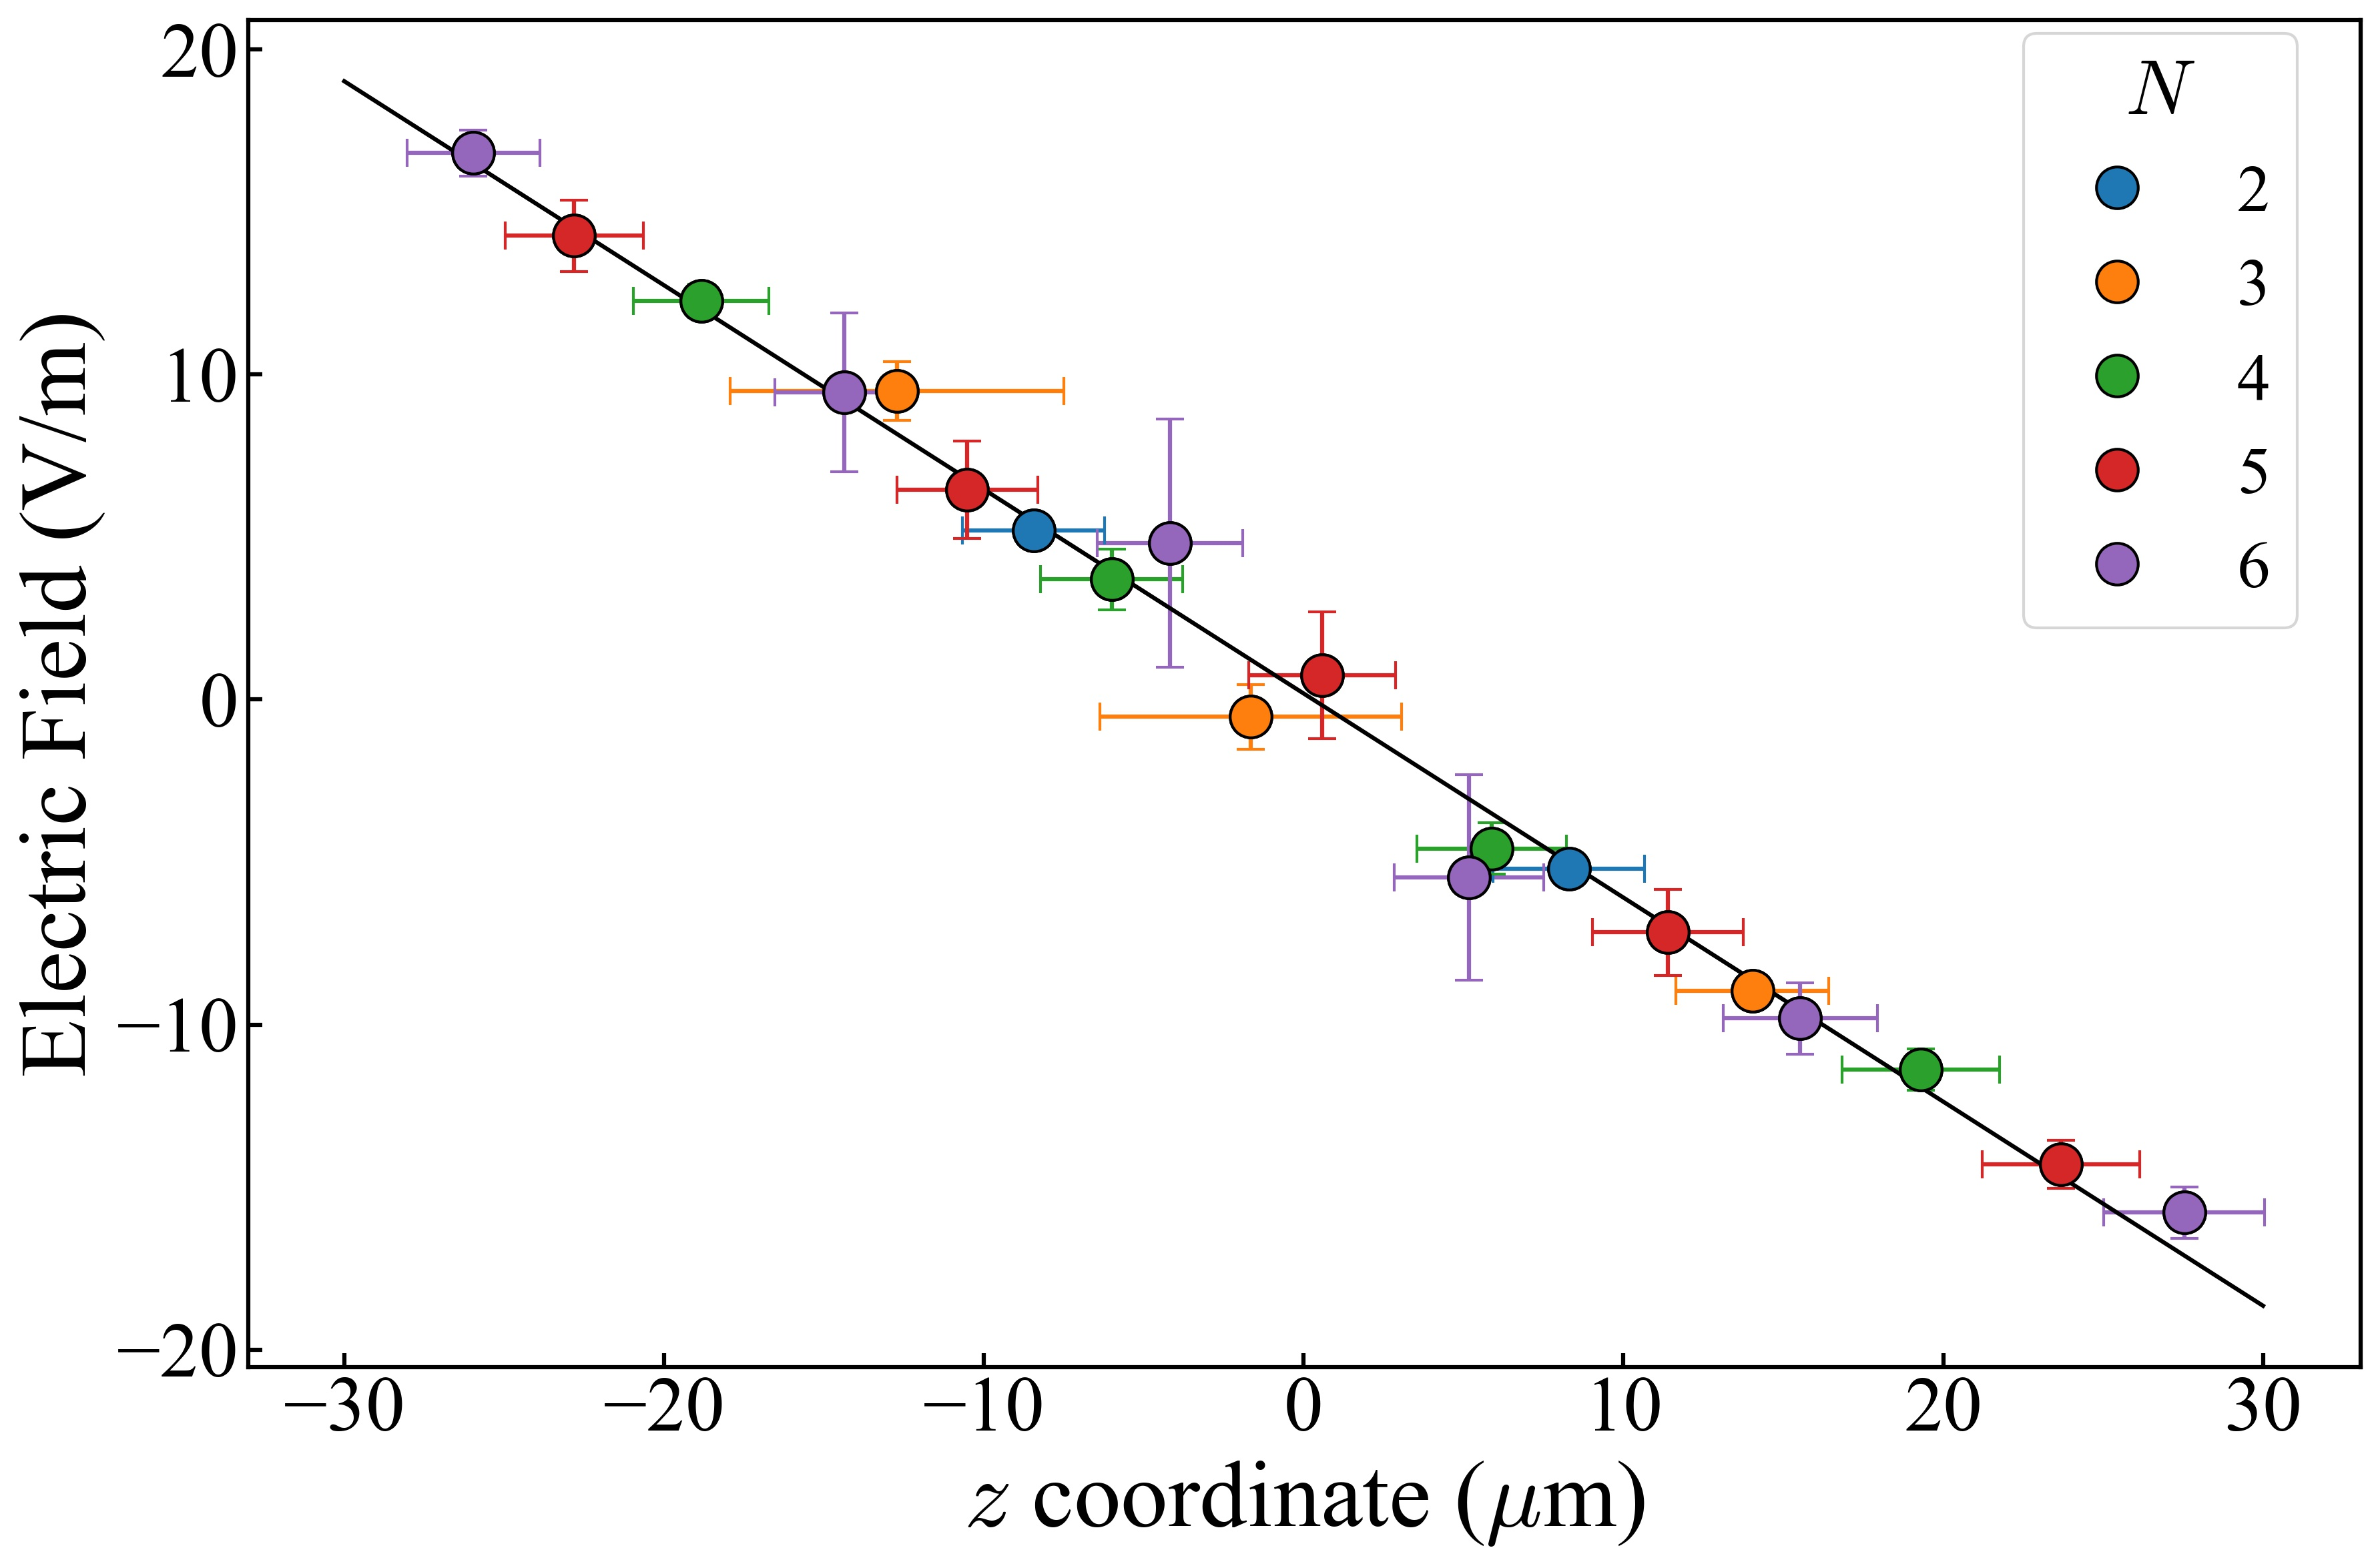
\includegraphics[width = 0.6\linewidth]{./results/figure/DC1_E.jpg}
		\caption{dc電圧セットDC1において$N \ = \ 1 \sim 6$としたときに算出されたイオン捕獲位置における電場の値とそのフィッティング結果}
		\label{fig:DC1_E}
	\end{center}
\end{figure}

dc電圧セットDC2,DC3の条件においても同様の実験を行い,一次関数によるフィッティングを施した結果を\Fig{DC2_E},\Fig{DC3_E}に示す.

\begin{figure}[h]
	\begin{center}
		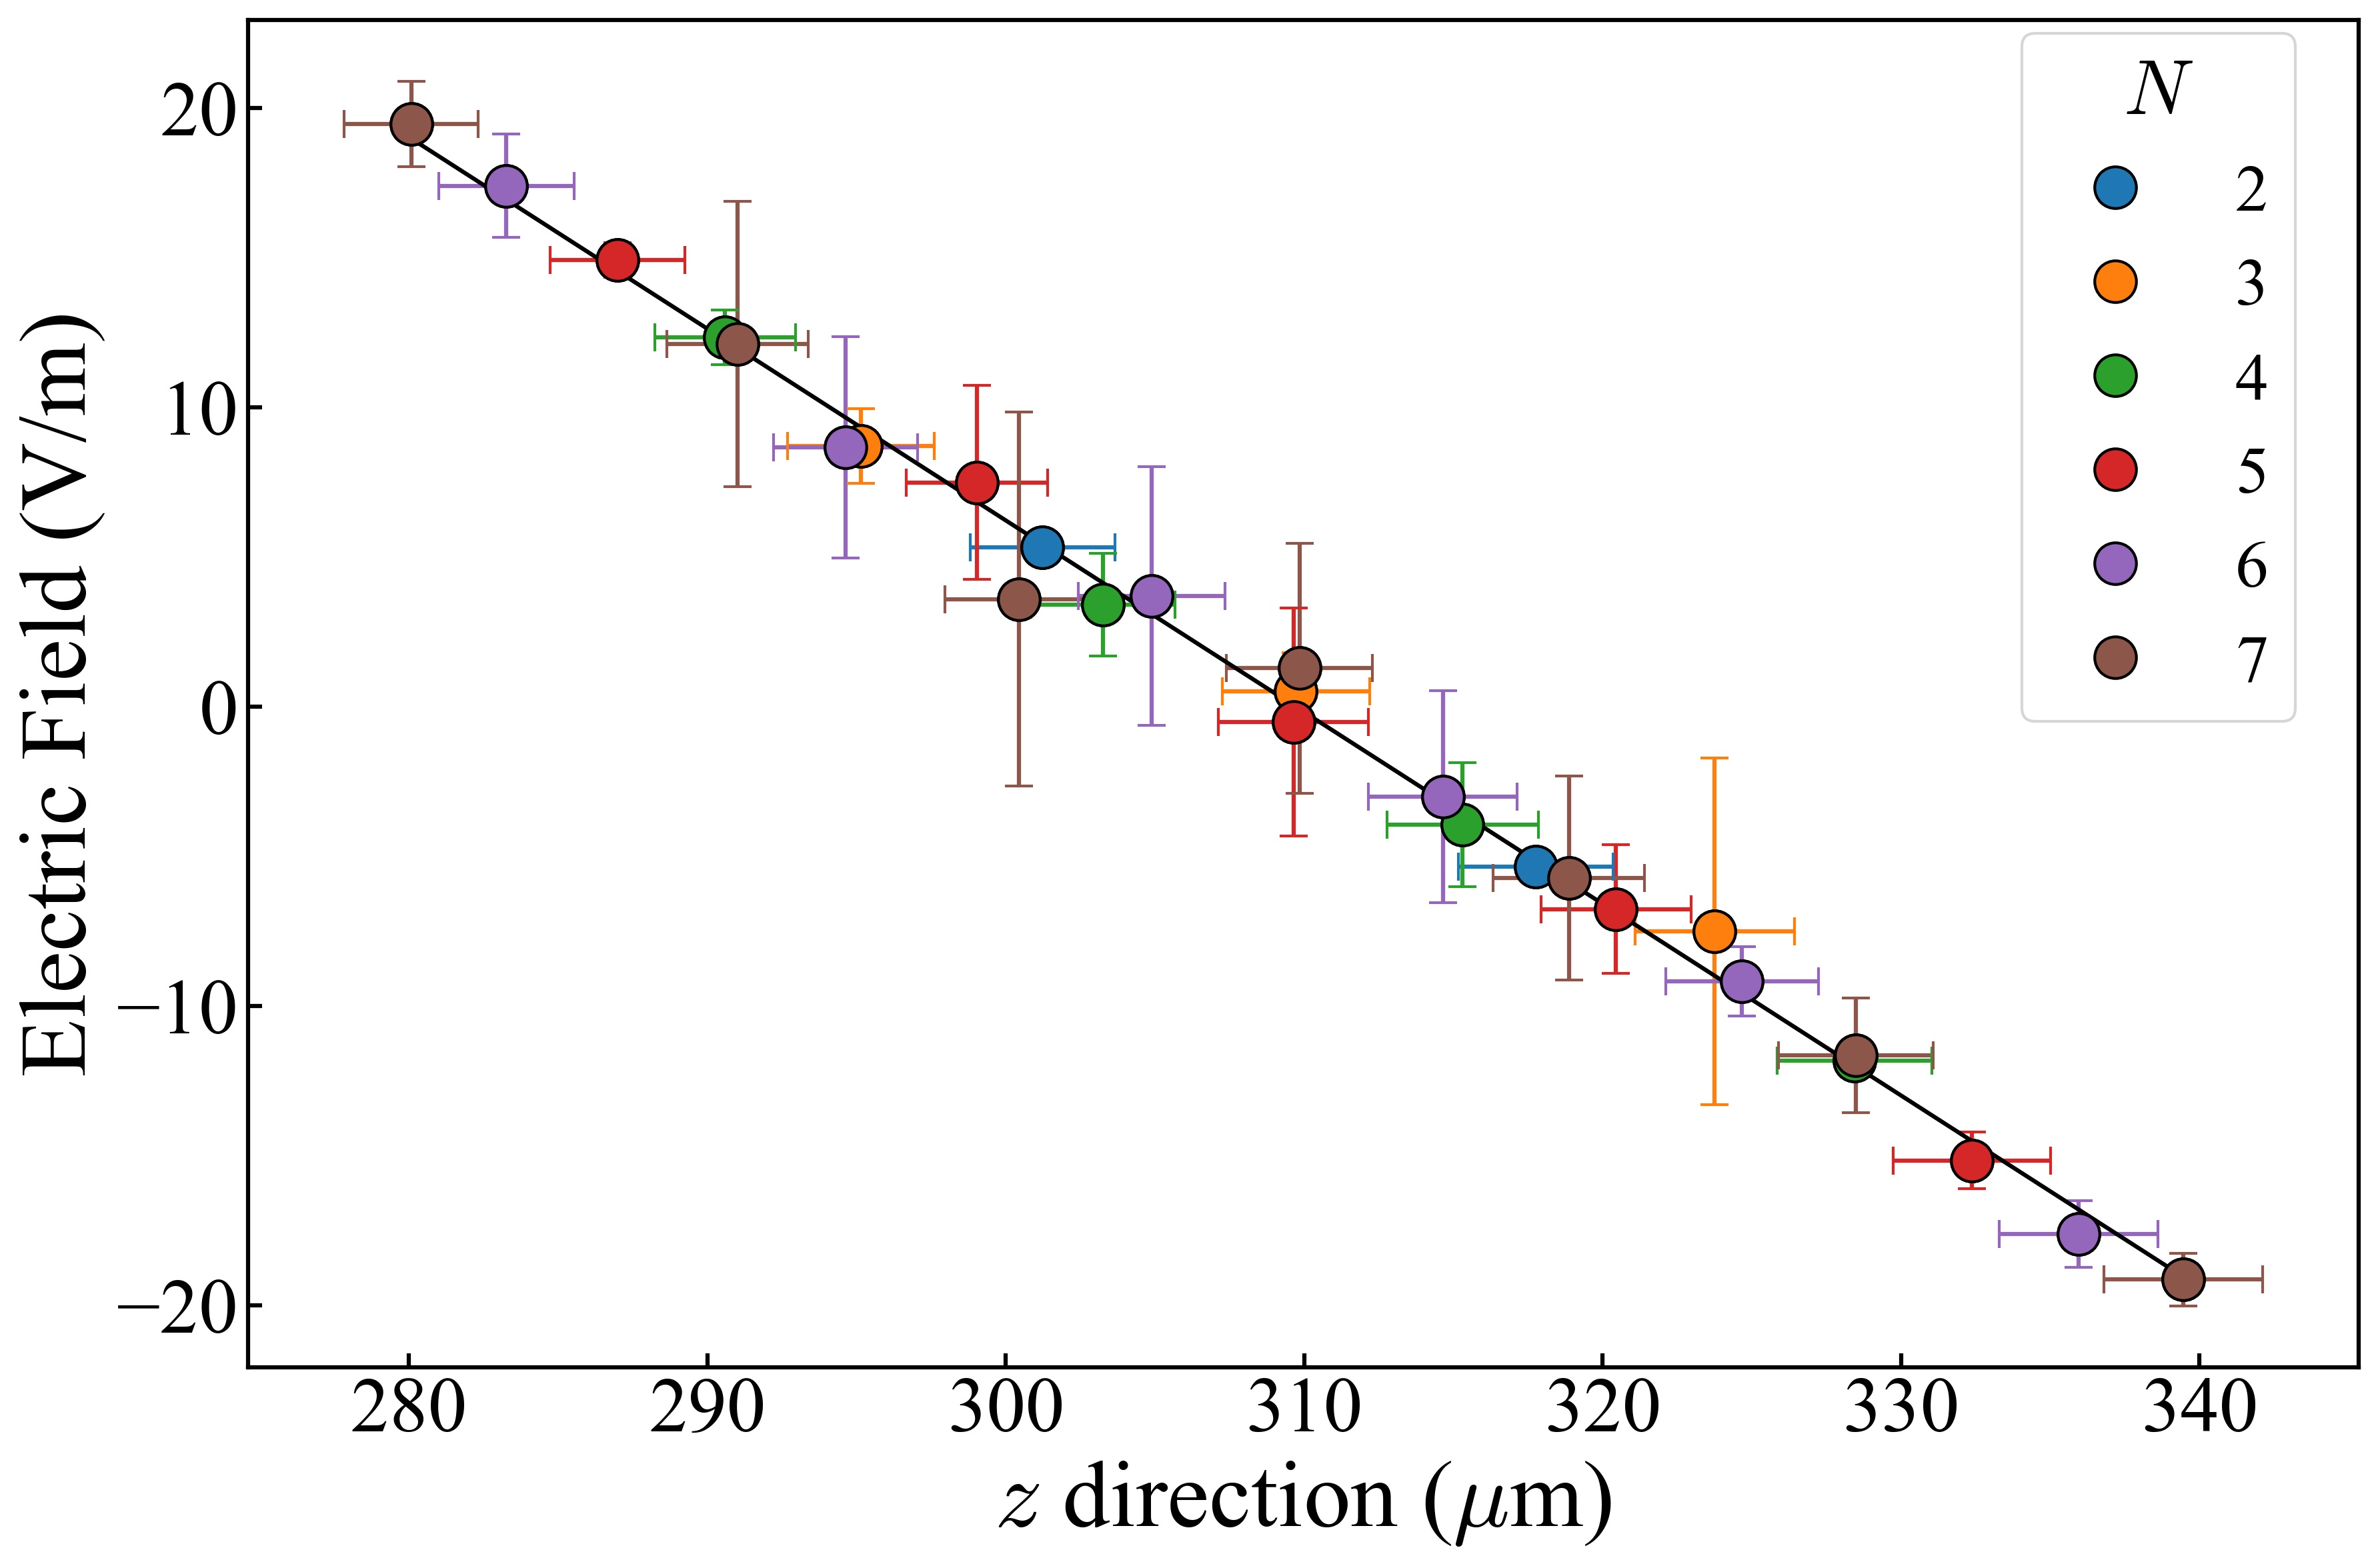
\includegraphics[width = 0.6\linewidth]{./results/figure/DC2_E.jpg}
		\caption{dc電圧セットDC2において$N \ = \ 1 \sim 7$としたときに算出されたイオン捕獲位置における電場の値とそのフィッティング結果}
		\label{fig:DC2_E}
	\end{center}
\end{figure}

\begin{figure}[h]
	\begin{center}
		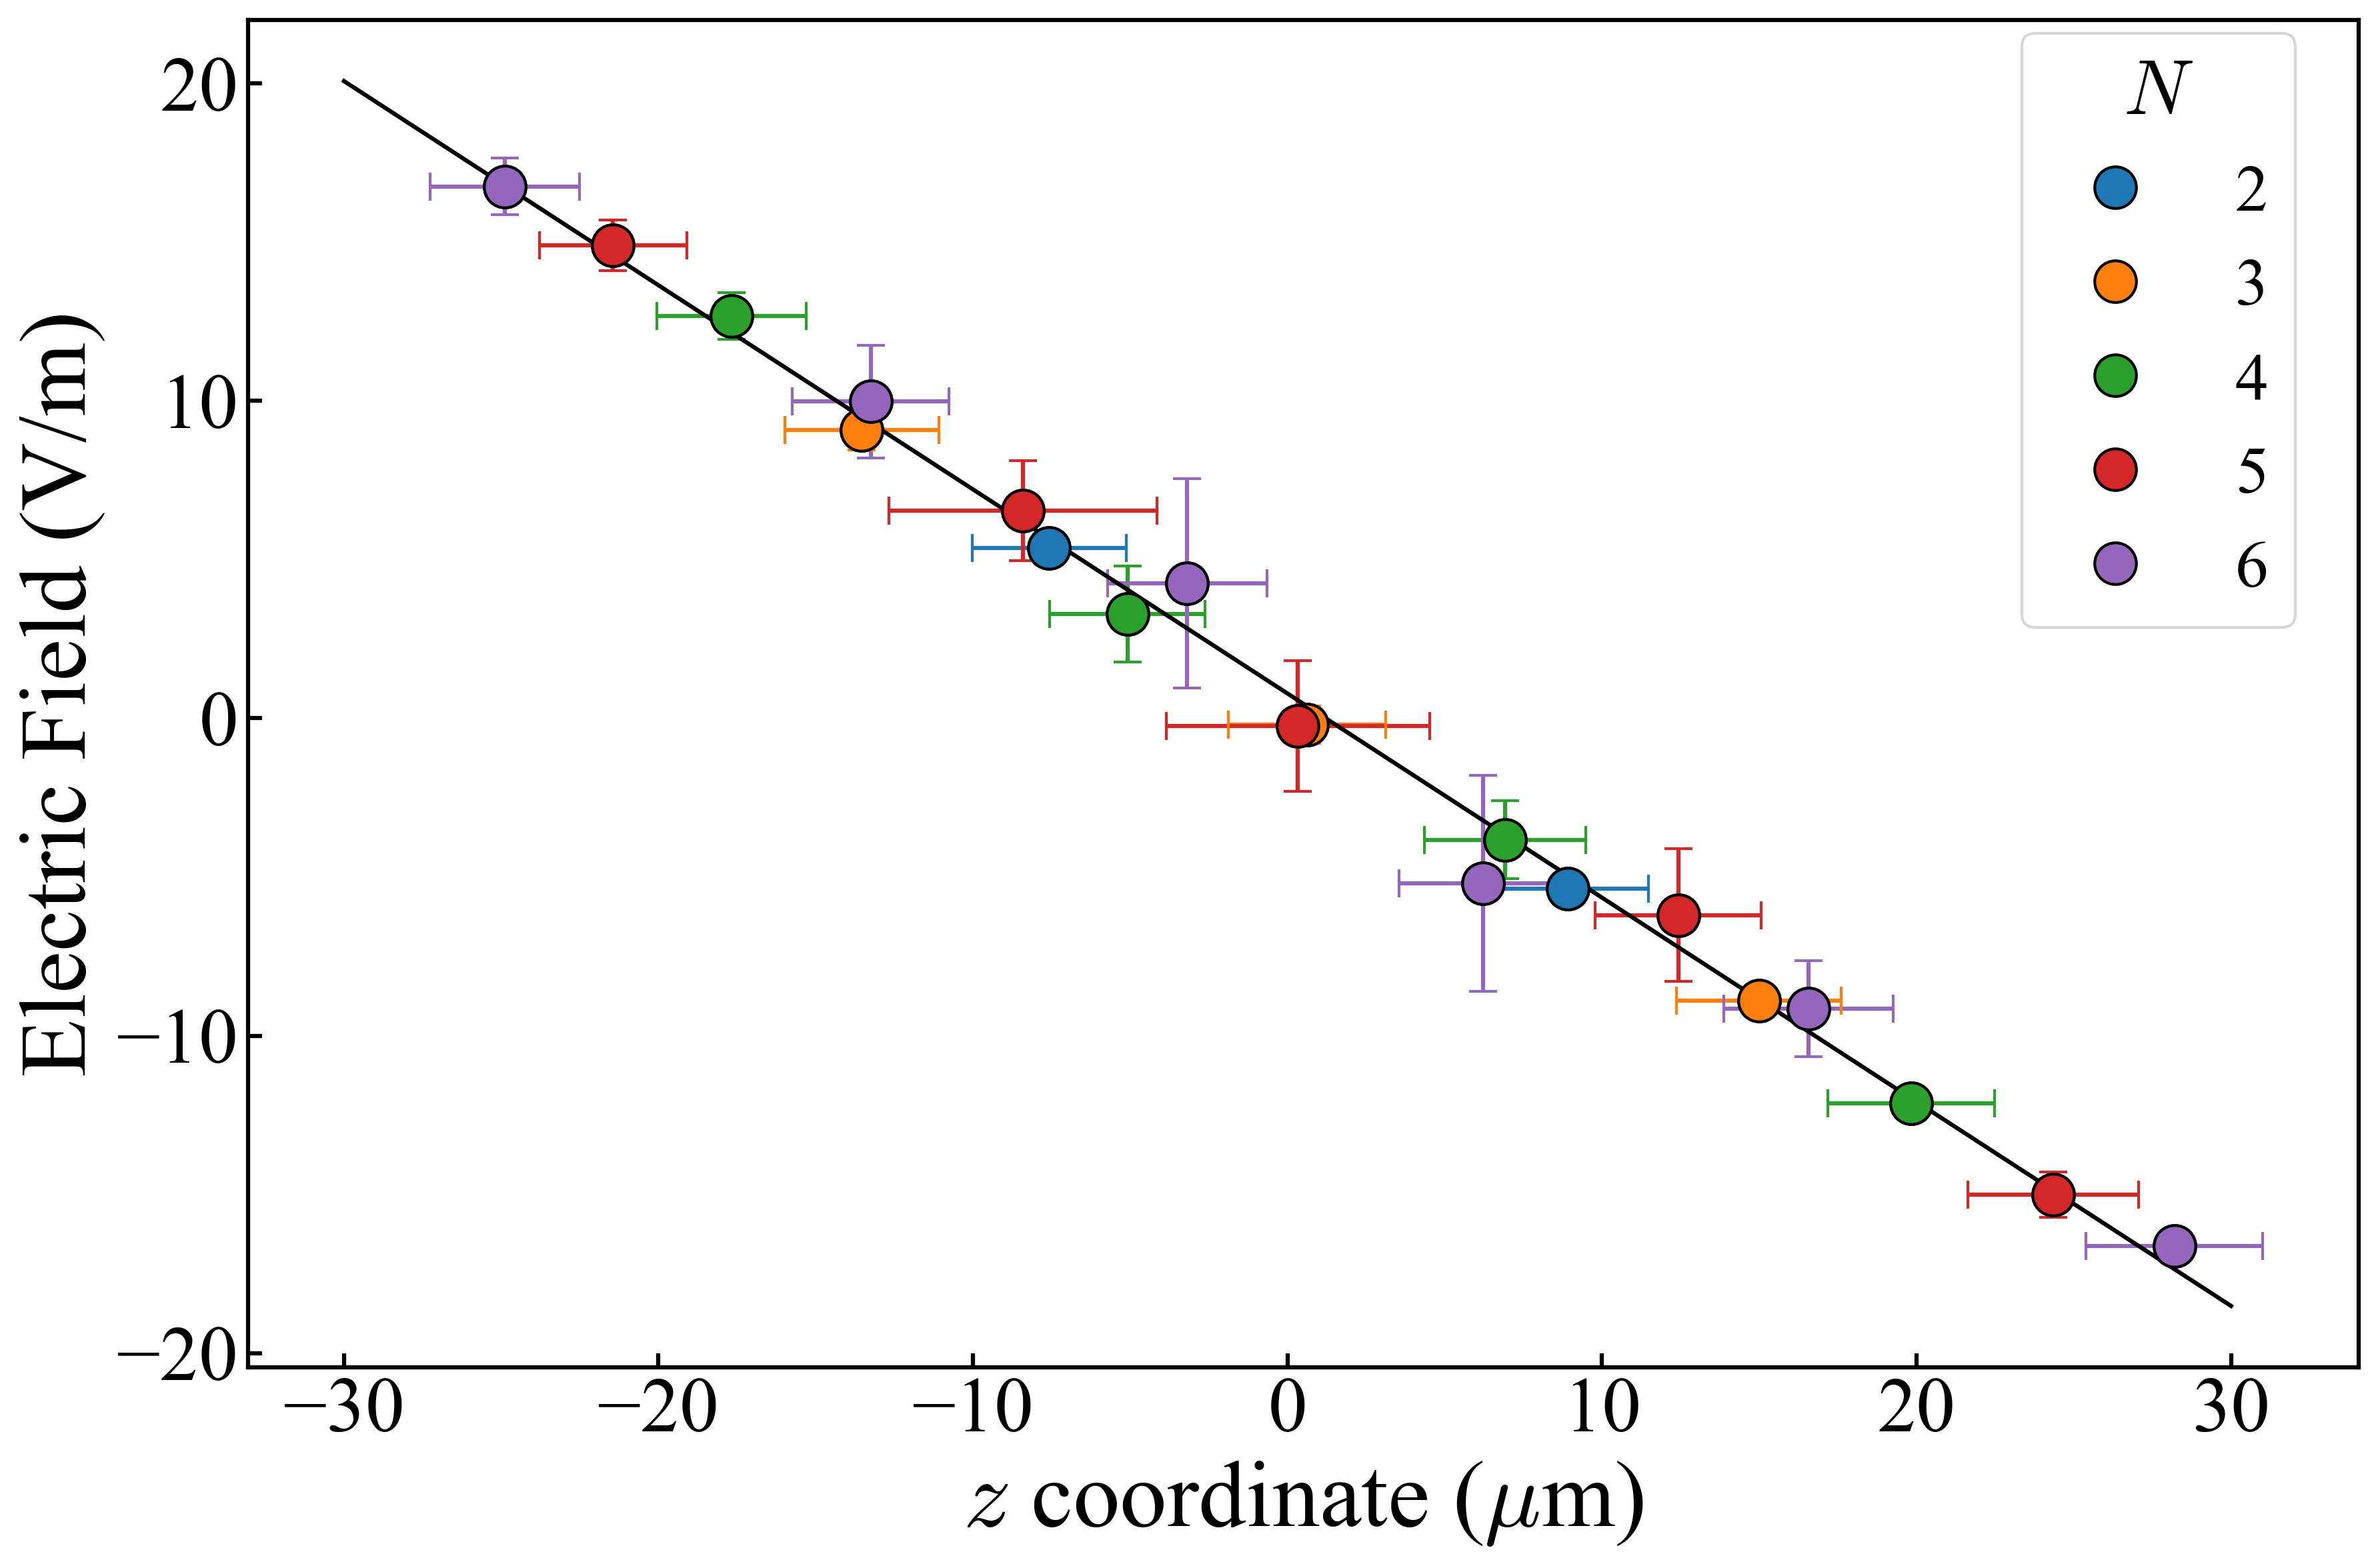
\includegraphics[width = 0.6\linewidth]{./results/figure/DC3_E.jpg}
		\caption{dc電圧セットDC3において$N \ = \ 1 \sim 6$としたときに算出されたイオン捕獲位置における電場の値とそのフィッティング結果}
		\label{fig:DC3_E}
	\end{center}
\end{figure}
%
\clearpage
%
\subsection{2通りの電場の傾きの算出方法の比較}

\begin{figure}[h]
	\begin{center}
		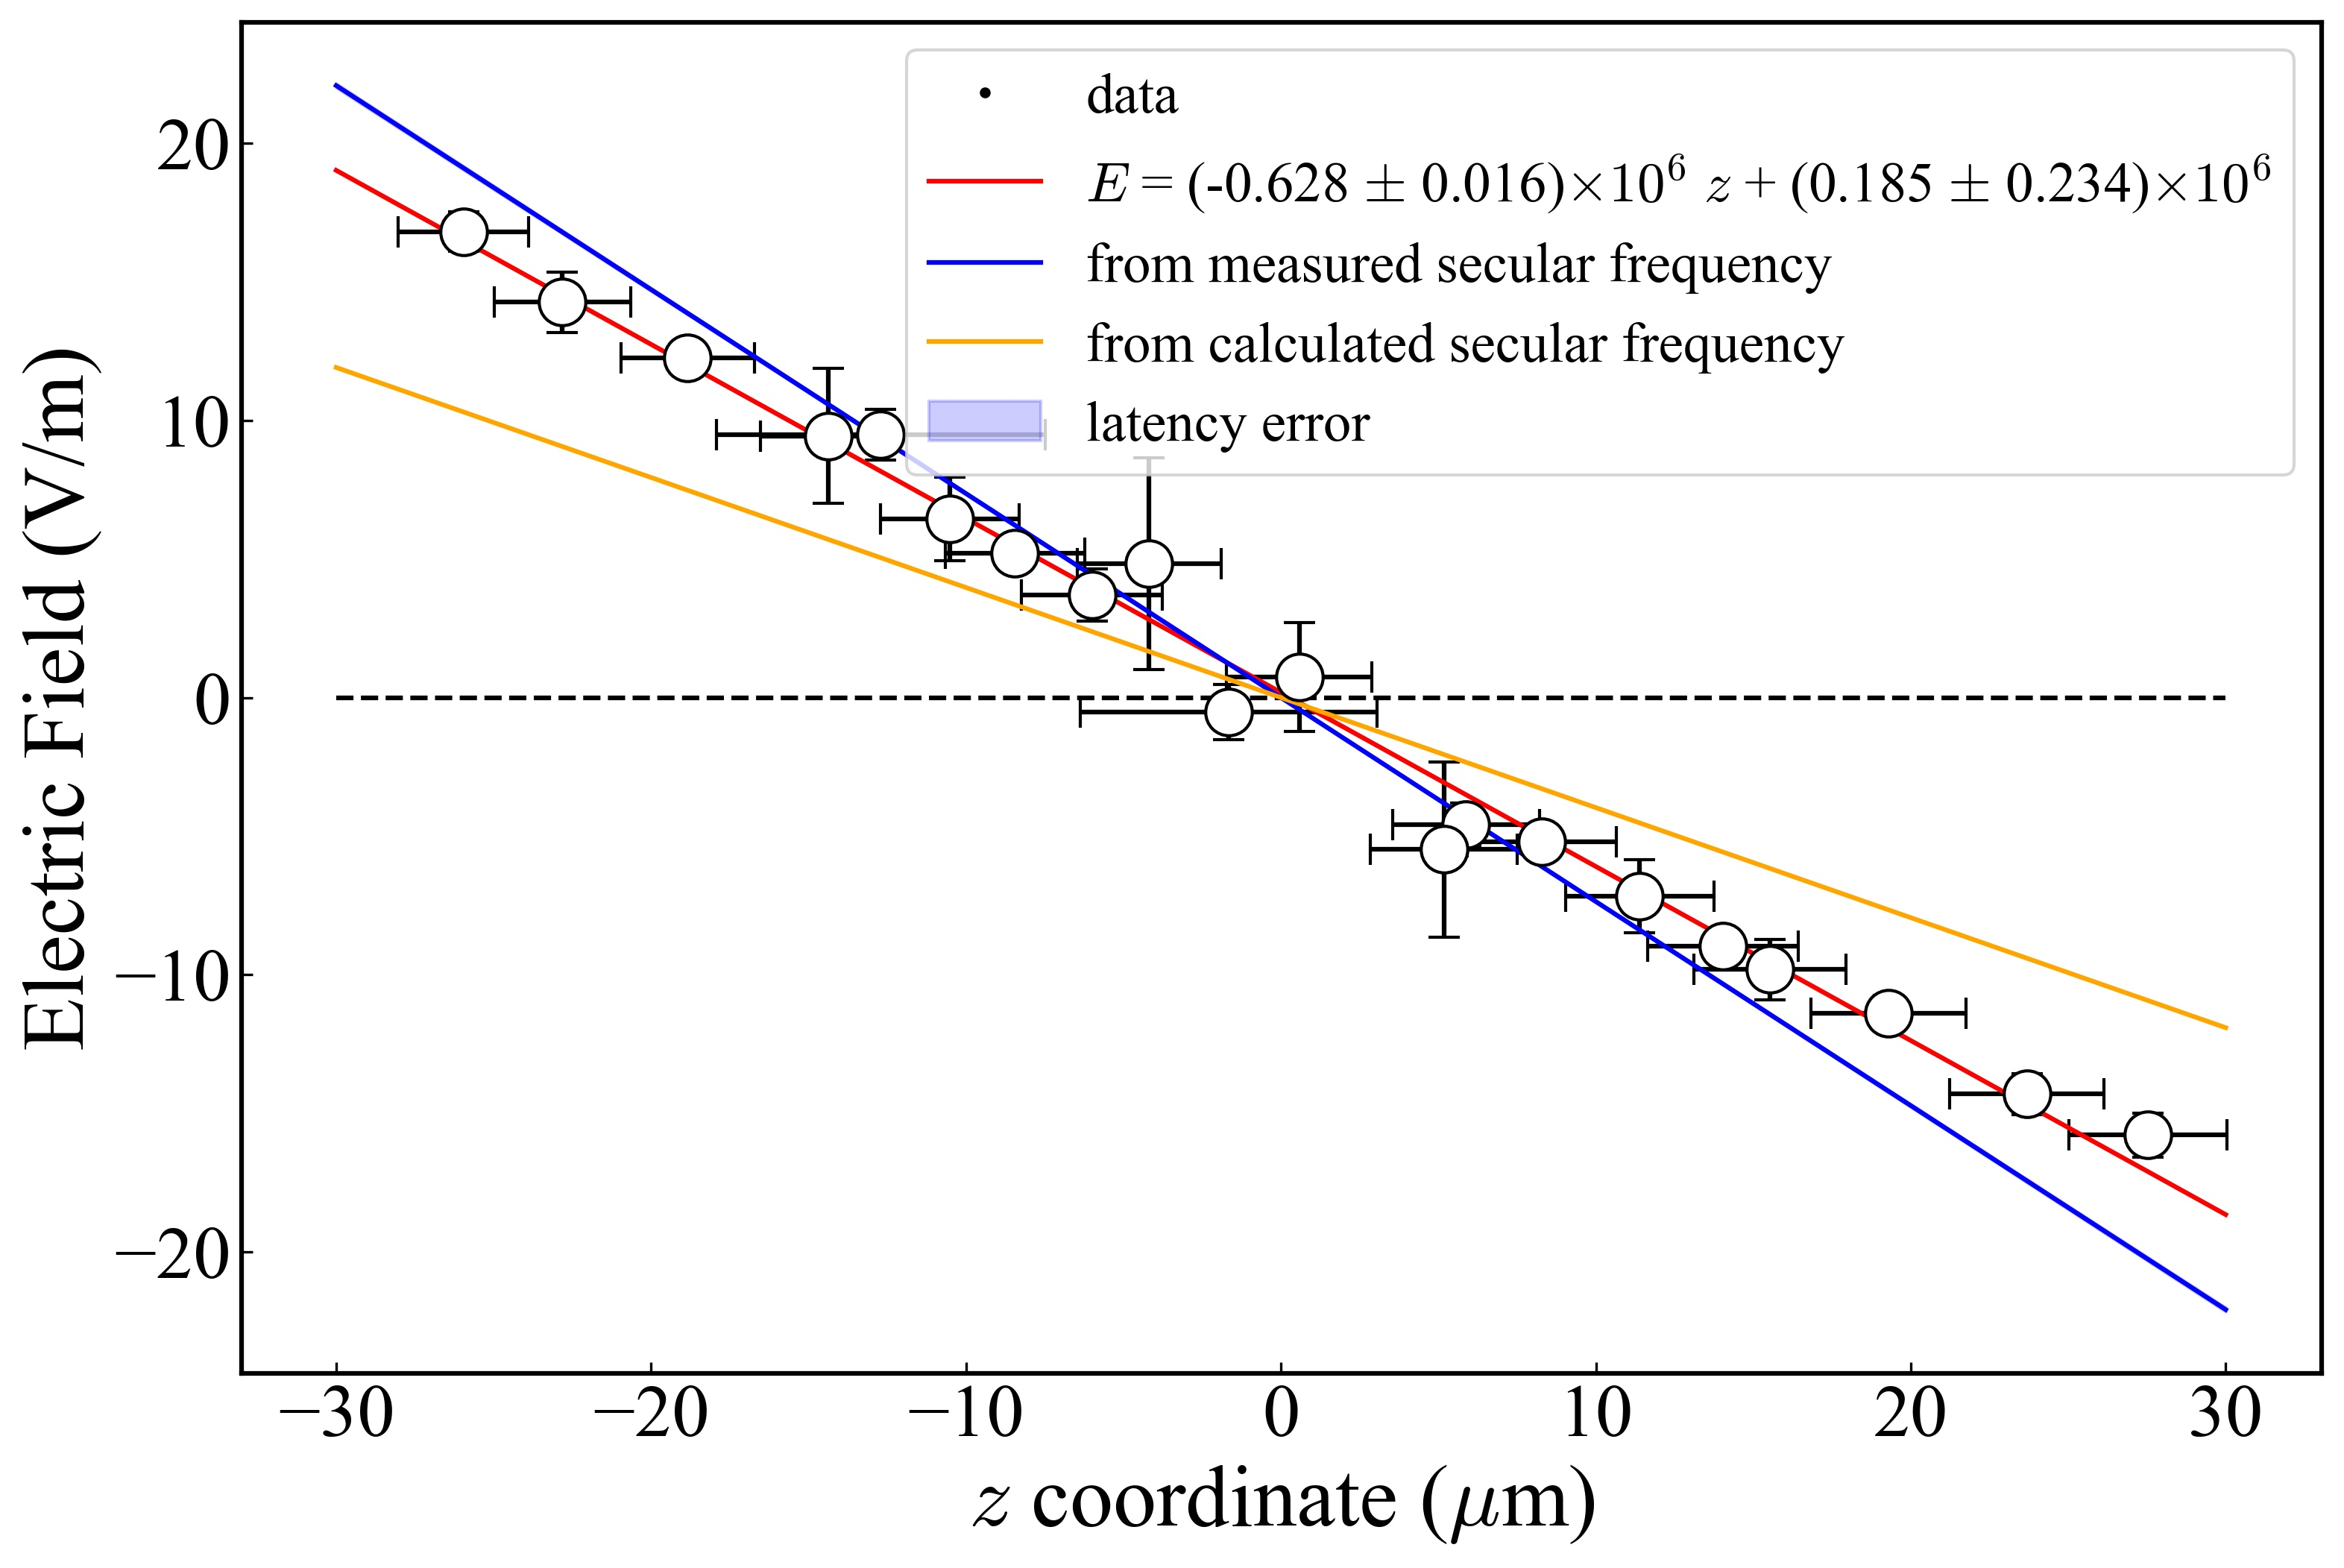
\includegraphics[width = 0.6\linewidth]{./results/figure/DC1_COMP.jpg}
		\caption{イオンの平衡位置から算出された電場から求められる電場の傾きと永年周波数のシミュレーション値と実験値から得られる電場の傾きの比較}
		\label{fig:DC1_COMP}
	\end{center}
\end{figure}
\begin{figure}[h]
	\begin{center}
		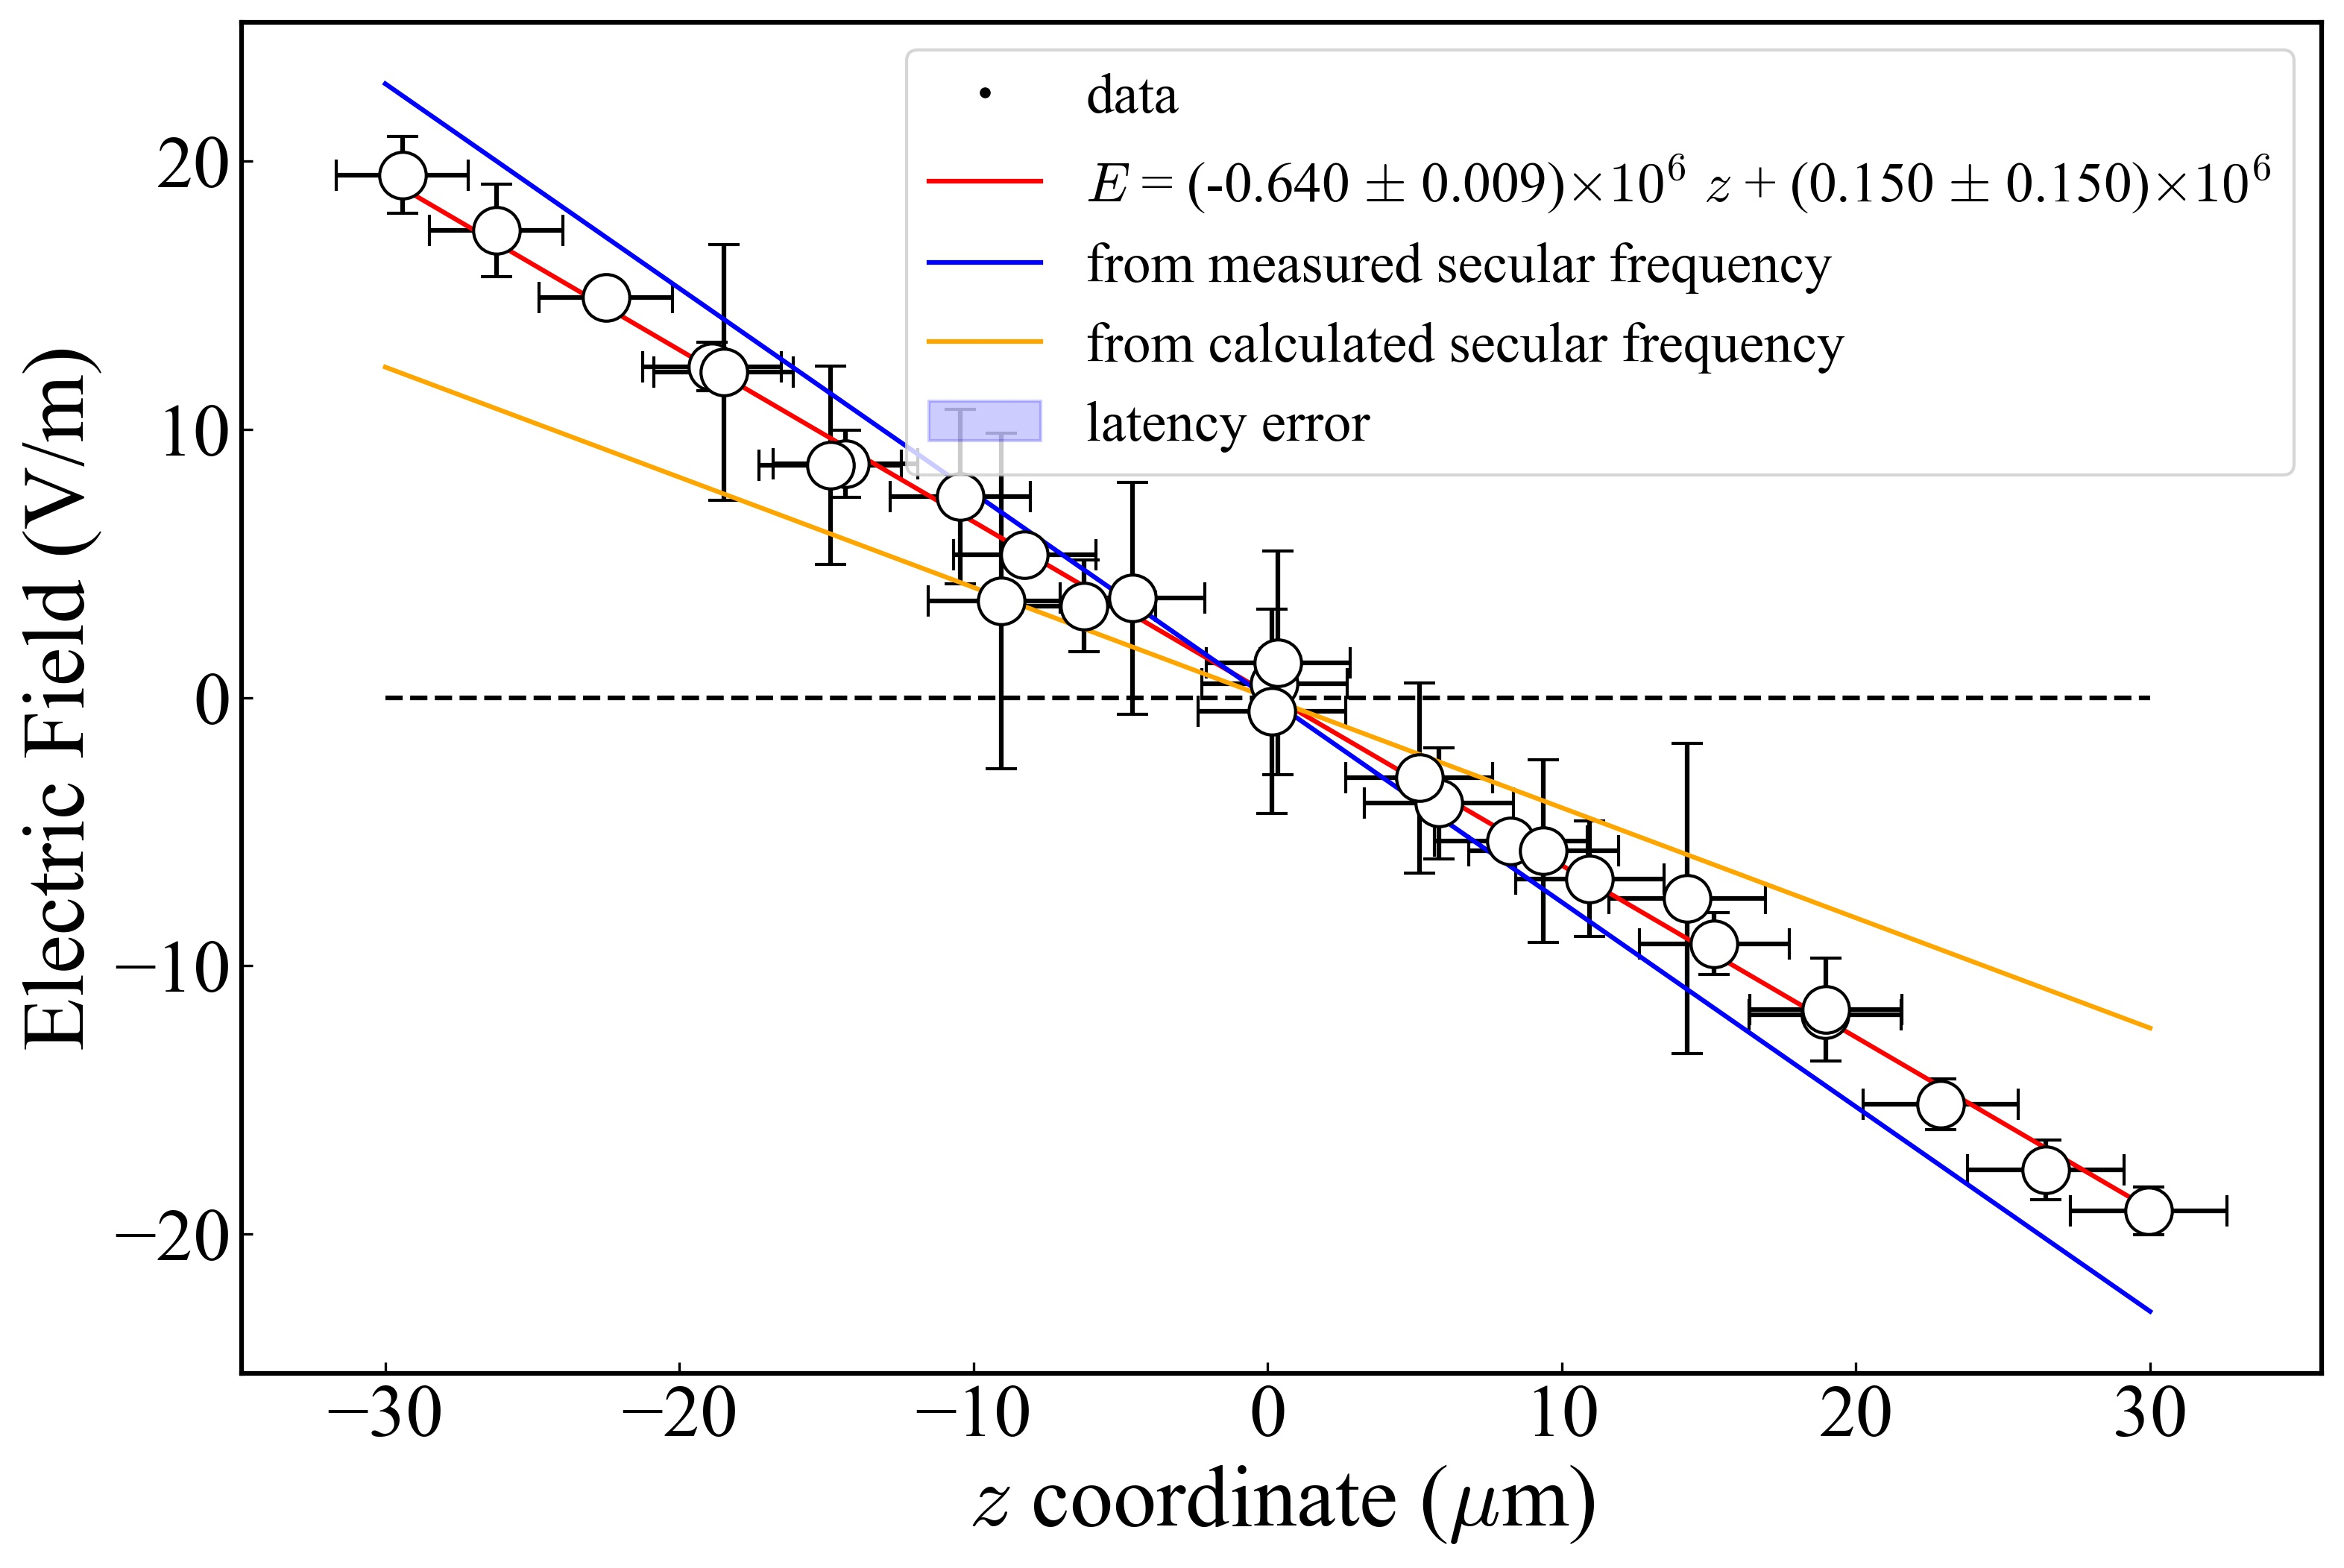
\includegraphics[width = 0.6\linewidth]{./results/figure/DC2_COMP.jpg}
		\caption{イオンの平衡位置から算出された電場から求められる電場の傾きと永年周波数のシミュレーション値と実験値から得られる電場の傾きの比較}
		\label{fig:DC2_COMP}
	\end{center}
\end{figure}
\begin{figure}[h]
	\begin{center}
		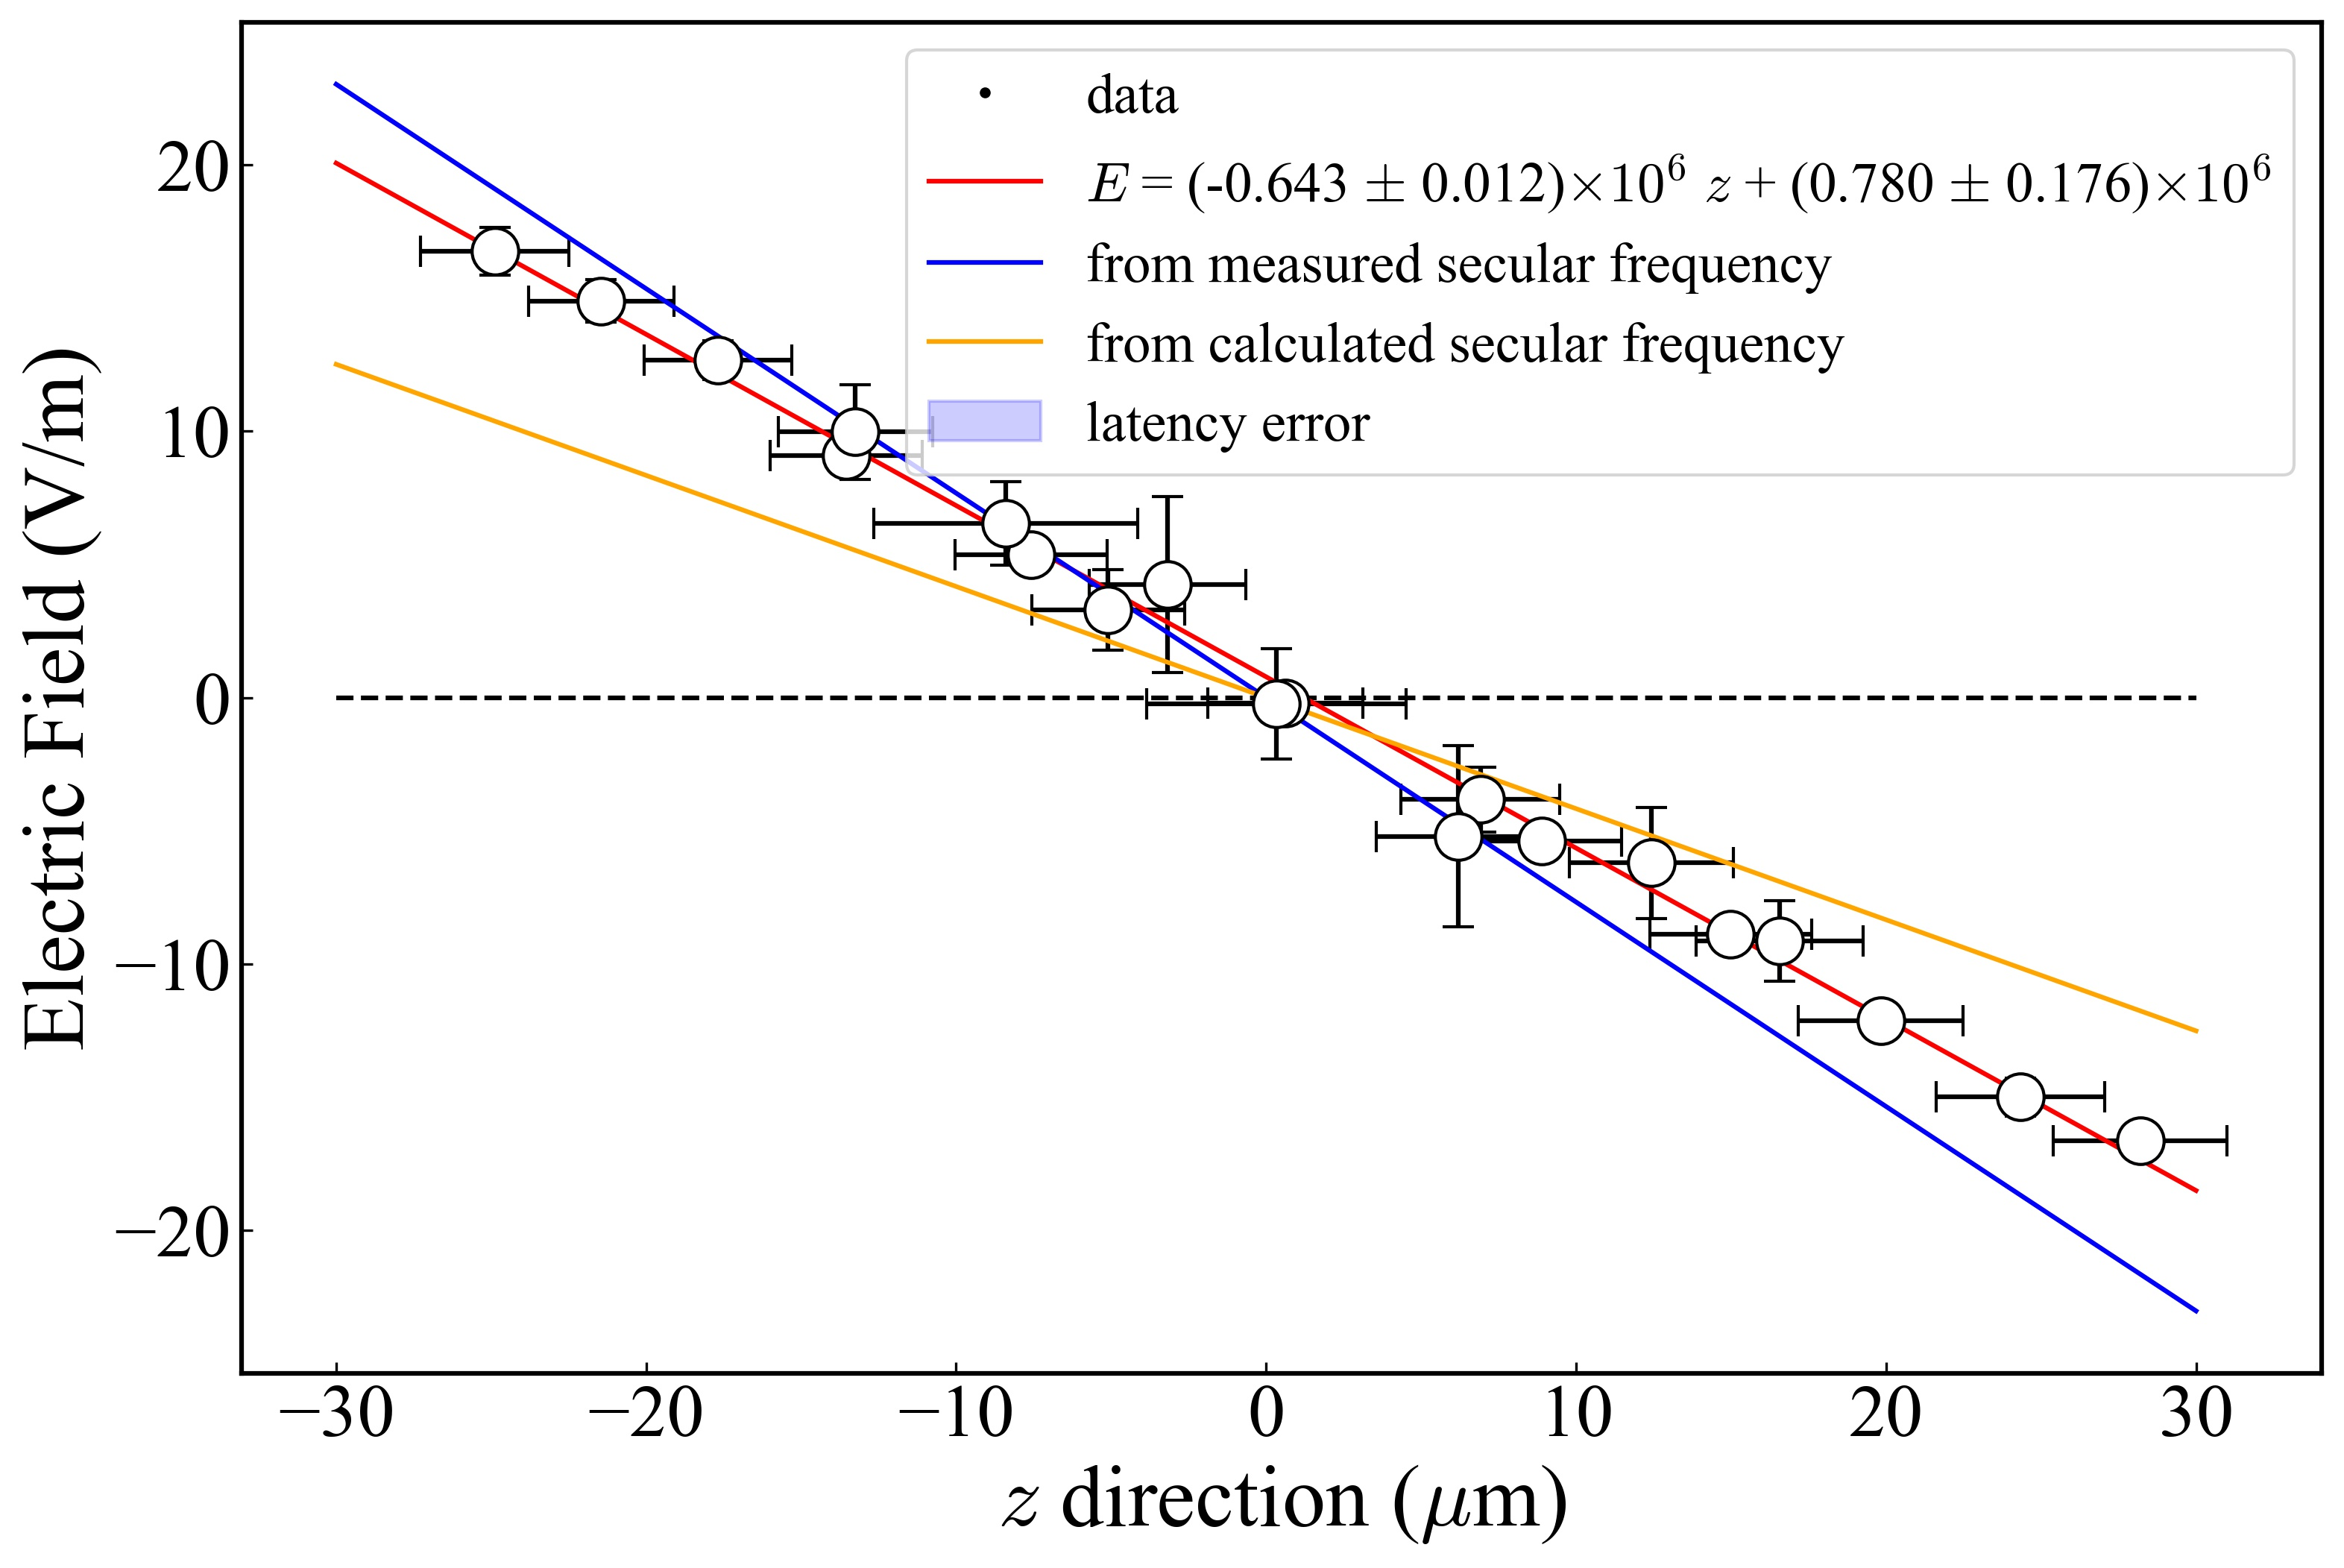
\includegraphics[width = 0.6\linewidth]{./results/figure/DC3_COMP.jpg}
		\caption{イオンの平衡位置から算出された電場から求められる電場の傾きと永年周波数のシミュレーション値と実験値から得られる電場の傾きの比較}
		\label{fig:DC3_COMP}
	\end{center}
\end{figure}

%
\clearpage
%
\section{二列配列イオン}
\subsection{イオン列間距離dと比率Rとの関係}
\subsection{永年周波数の測定結果}

\begin{figure}[h]
	\begin{minipage}{0.5\linewidth}
		\begin{center}
			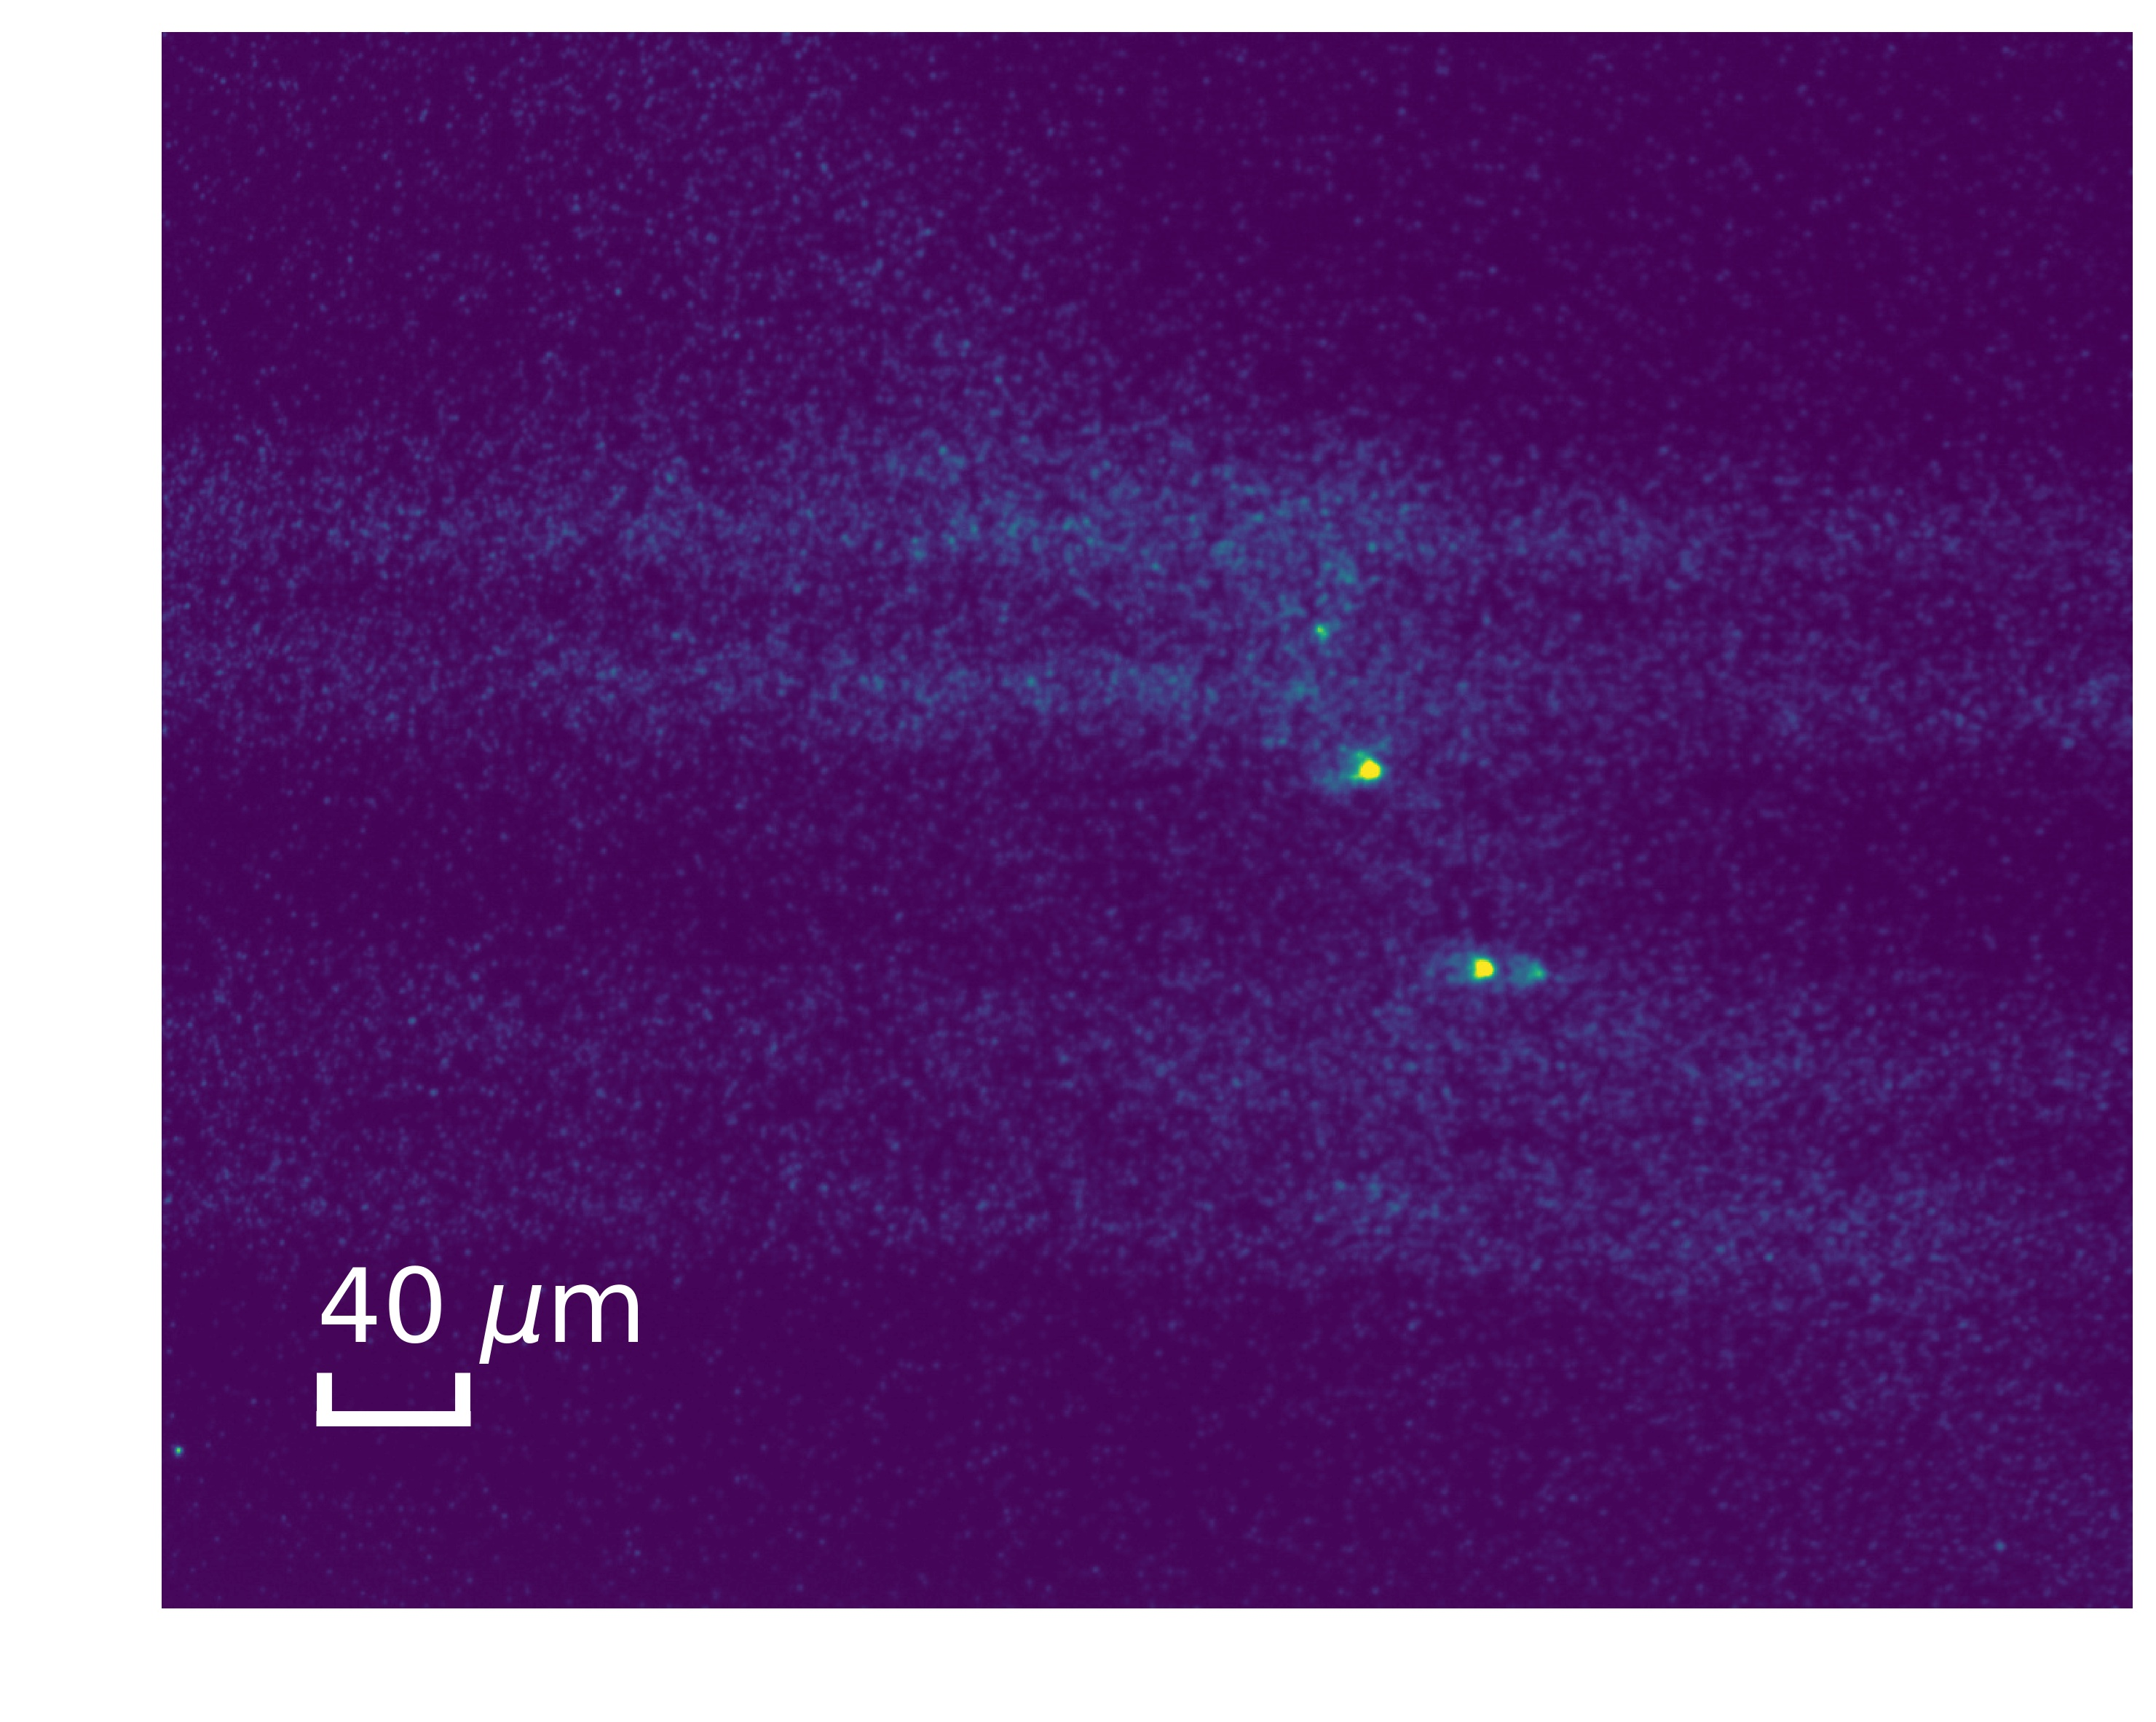
\includegraphics[width = 0.98\columnwidth]{./results/figure/2D_off_resonance.jpg}
			\caption{二列配列イオンでの非共鳴時の捕獲画像}
			\label{fig:2D_off_resonance}
		\end{center}
	\end{minipage}
	\begin{minipage}{0.5\linewidth}
		\begin{center}
			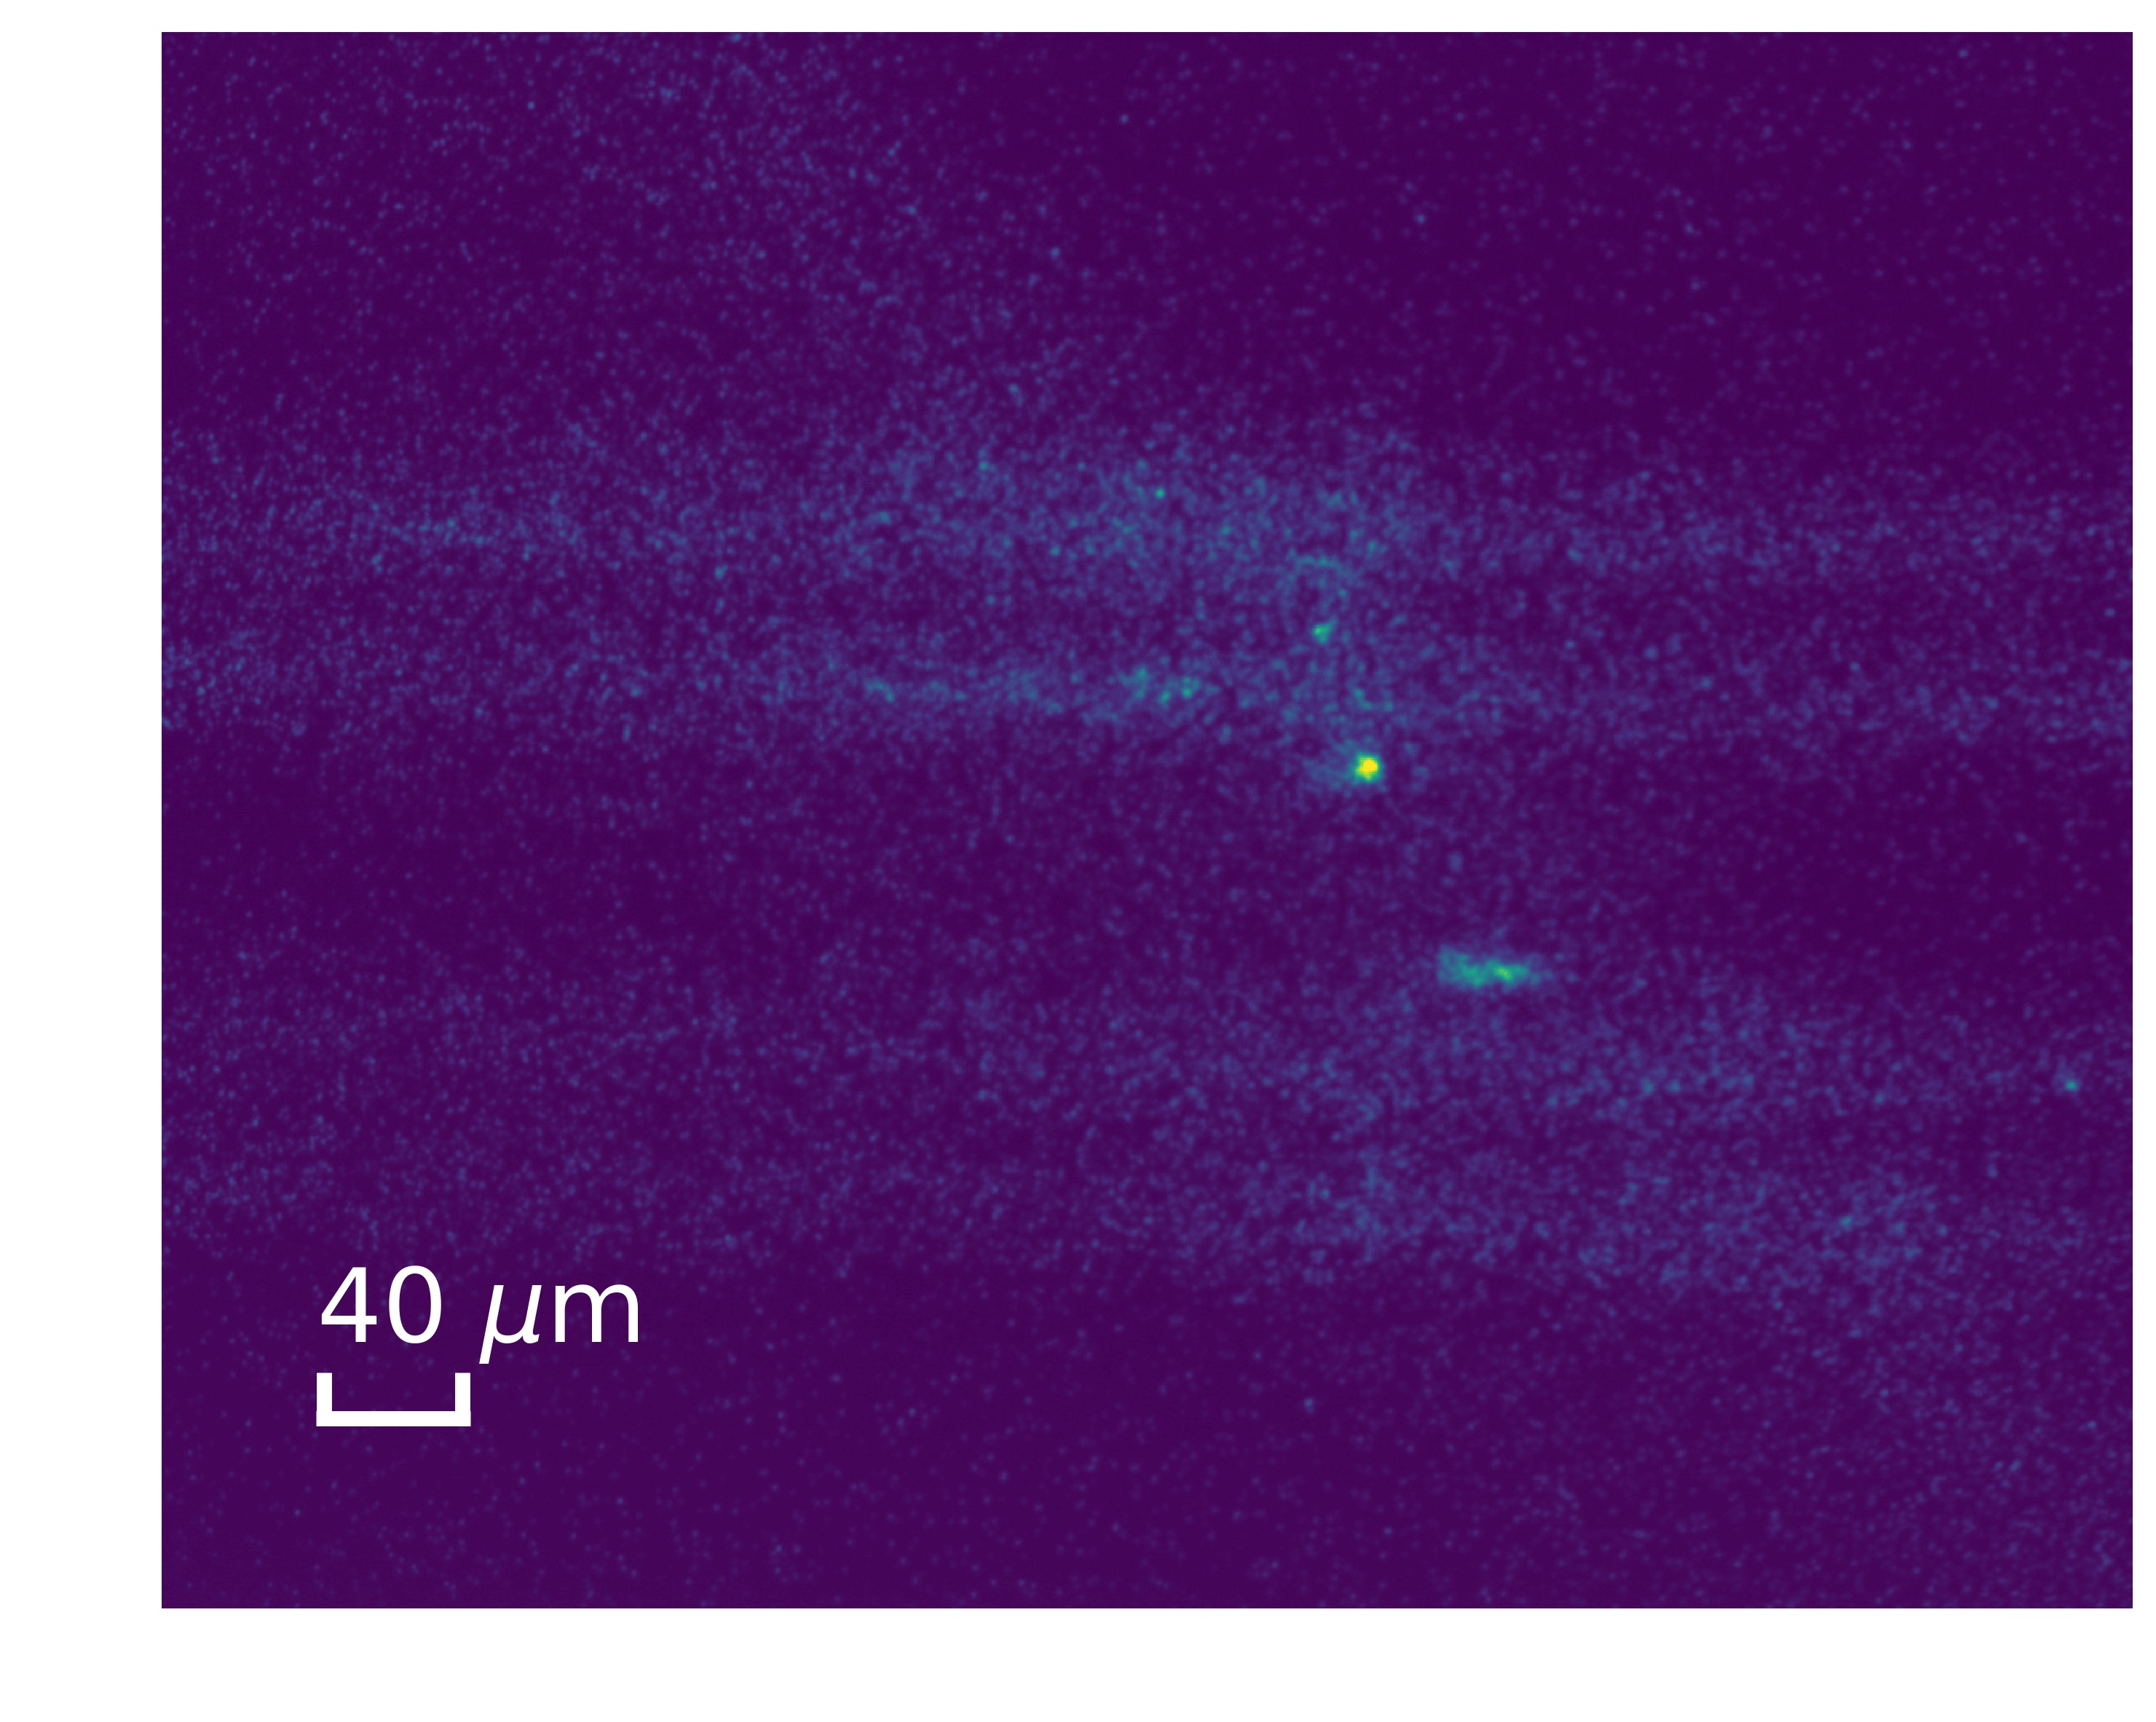
\includegraphics[width = 0.98\columnwidth]{./results/figure/2D_resonance.jpg}
			\caption{二列配列イオンでの共鳴時の捕獲画像}
			\label{fig:2D_resonance}
		\end{center}
	\end{minipage}
\end{figure}